%*******************************************************************************
%****************************** Appendix D *************************************
%*******************************************************************************
\chapter{Additional Results for HII experiment} \label{appendix:d}


% **************************** Define Graphics Path **************************
\graphicspath{{figs/appendixD/PDF/}}



\section{Time Series} \label{appendix:d:ts}
Time series for horizontal arm movements 
(Figs \ref{fig:tssg0gyroZ-hii}, 
\ref{fig:tssg1gyroZ-hii}, and \ref{fig:tssg2gyroZ-hii})
and vertical arm movements 
(Figs \ref{fig:tssg0gyroY-hii}, \ref{fig:tssg1gyroY-hii},
\ref{fig:tssg2gyroY-hii}).
Both time series are only for a window size of 500 samples length.
For the remained window size lengths of time series data, we refer
the reader to download the data and code at \cite{hwum2018}.
%%---------------------------------(FIGURE)-------------------------------------
\begin{figure}
\centering
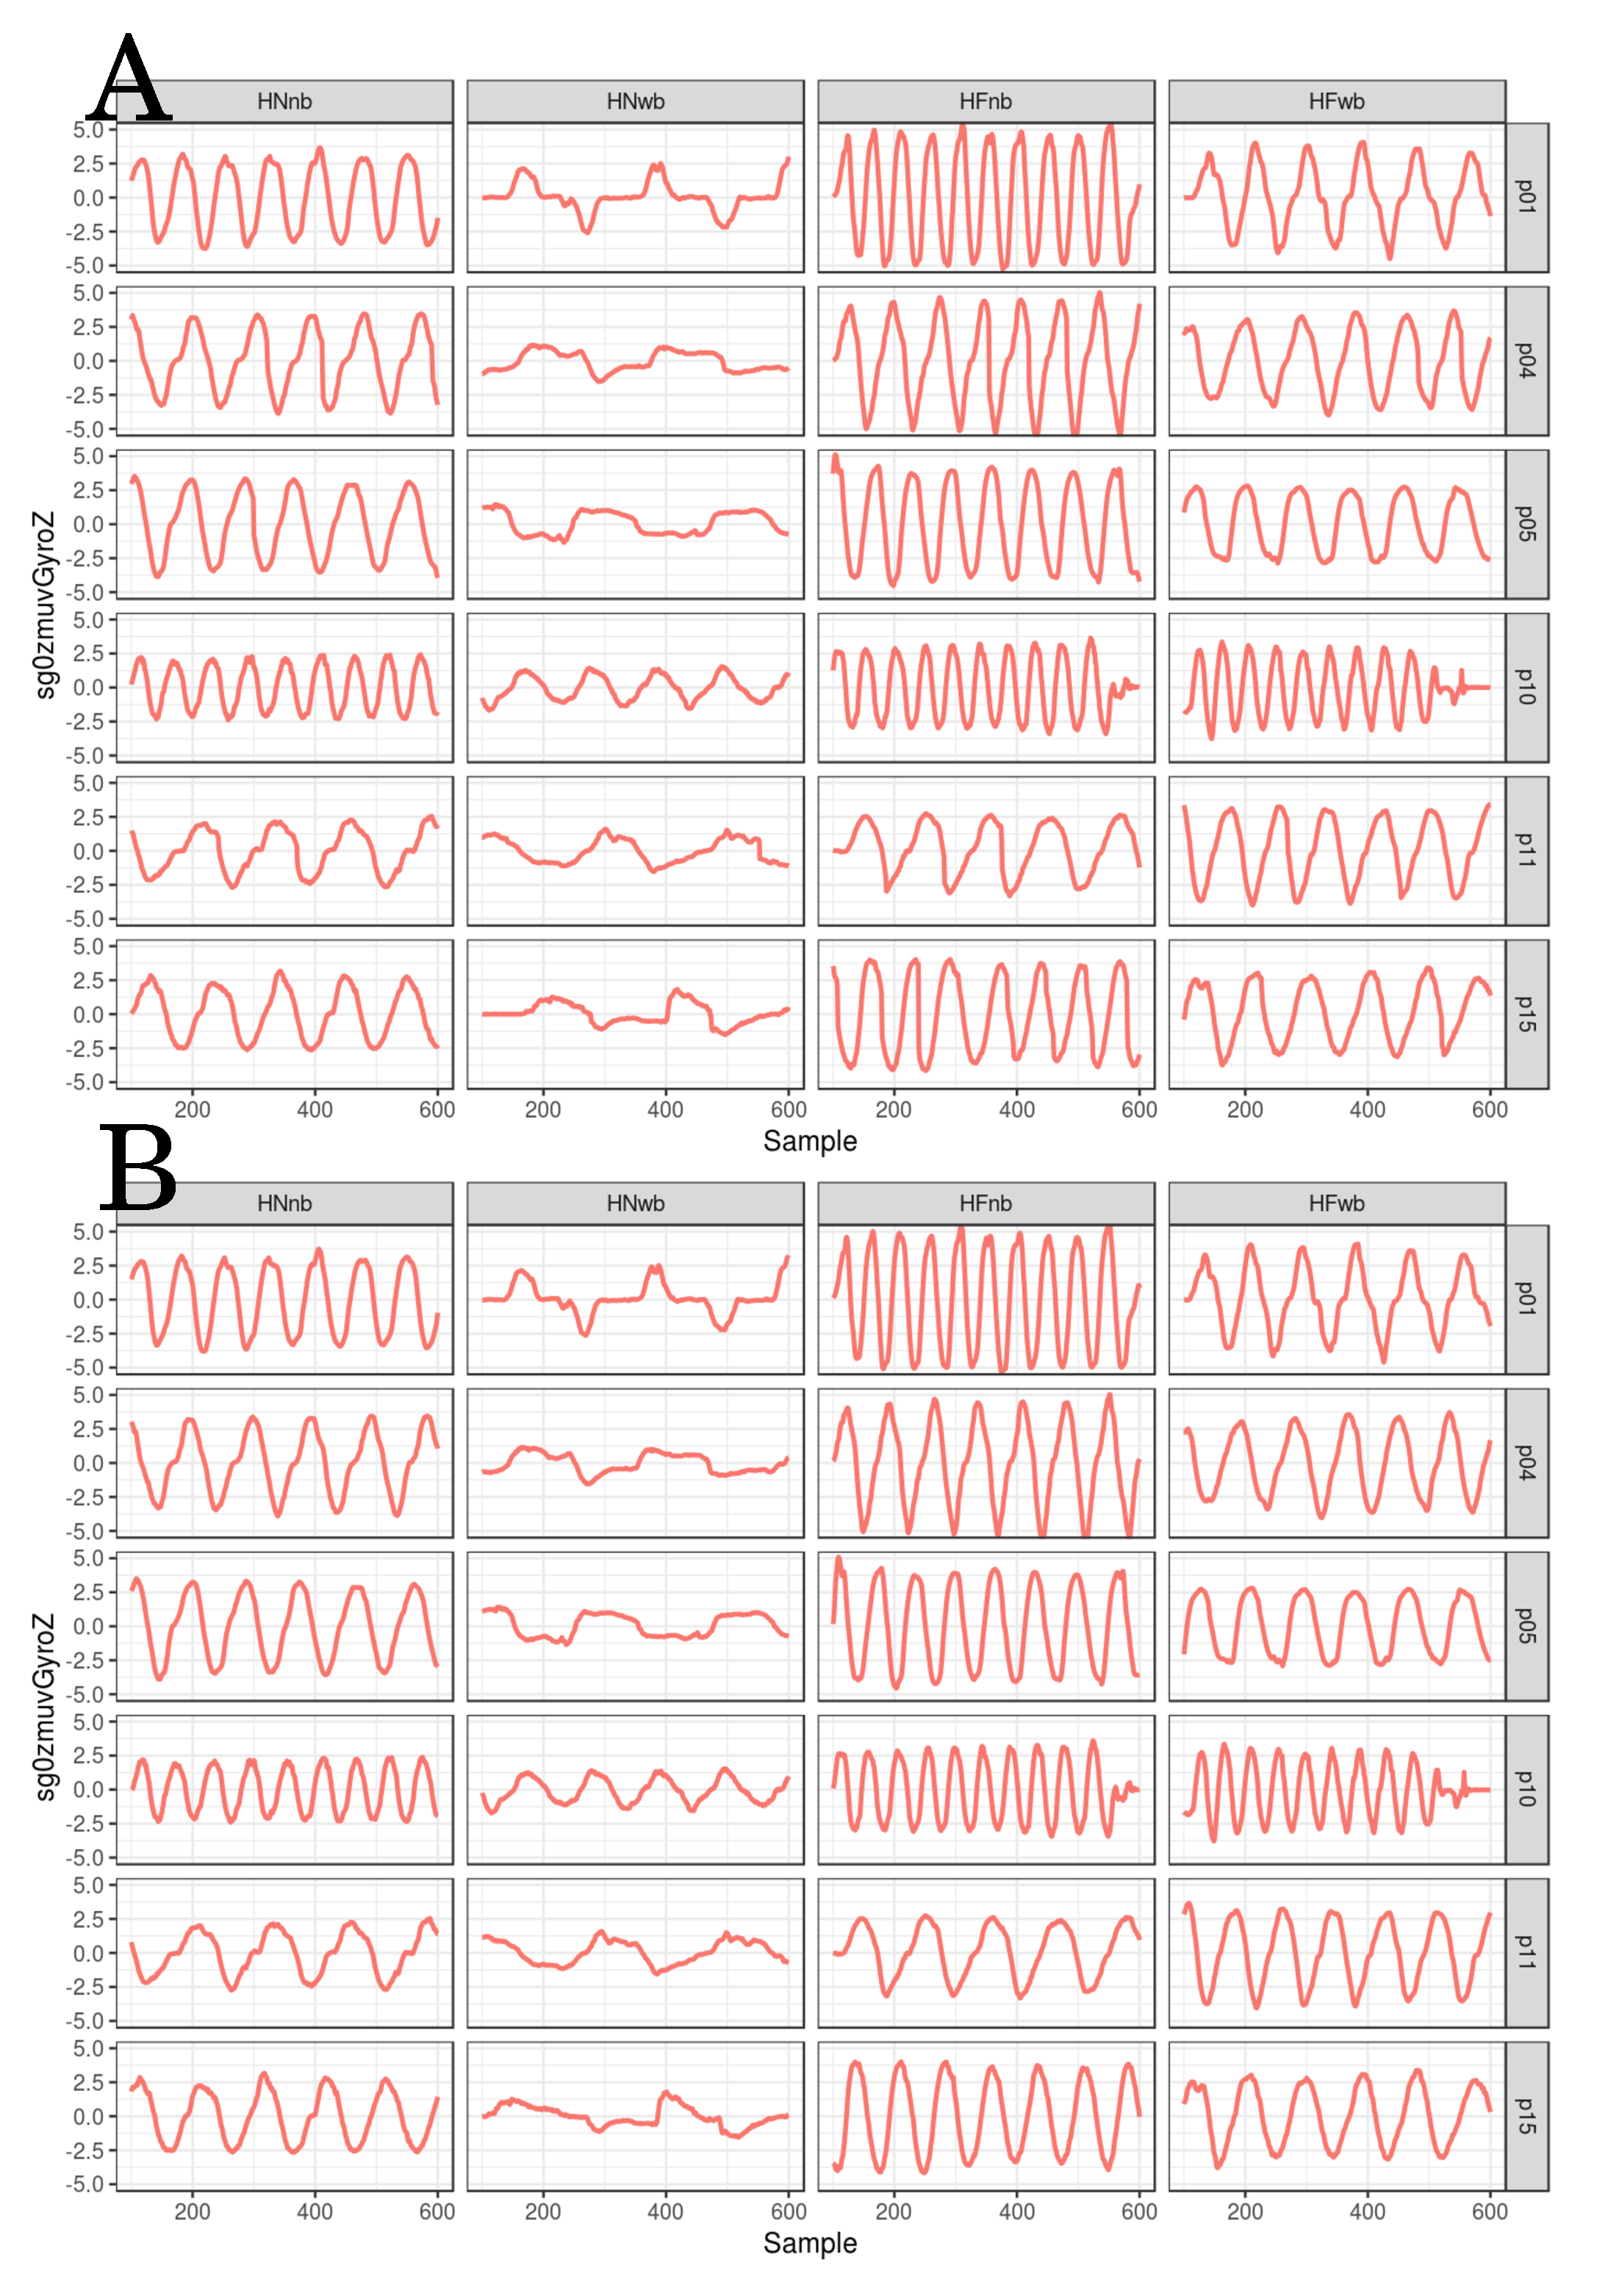
\includegraphics[width=0.8\textwidth]{tssg0gyroZ}
    	\caption
	[Time series for horizontal arm movements (sg0) ]{
	{\bf Time series for horizontal arm movements (sg0)}
		Time series for sg0GyroZ  are for six participants 
		($p01$, $p04$, $p05$, $p10$, $p11$, $p15$) 
		for horizontal movements in normal and faster velocity with
		no beat	(HNnb, HFnb) and with beat (HNwb, HFwb) using 
		the normalised GyroZ axis (zmuvGyroZ) and 
		two sensors attached to the participant wrist (HS01, HS02).
	R code to reproduce the figure is available from \cite{hwum2018}.
        }
    \label{fig:tssg0gyroZ-hii}
\end{figure}
%%---------------------------------(FIGURE)-----------------------------------


%%---------------------------------(FIGURE)-------------------------------------
\begin{figure}
\centering
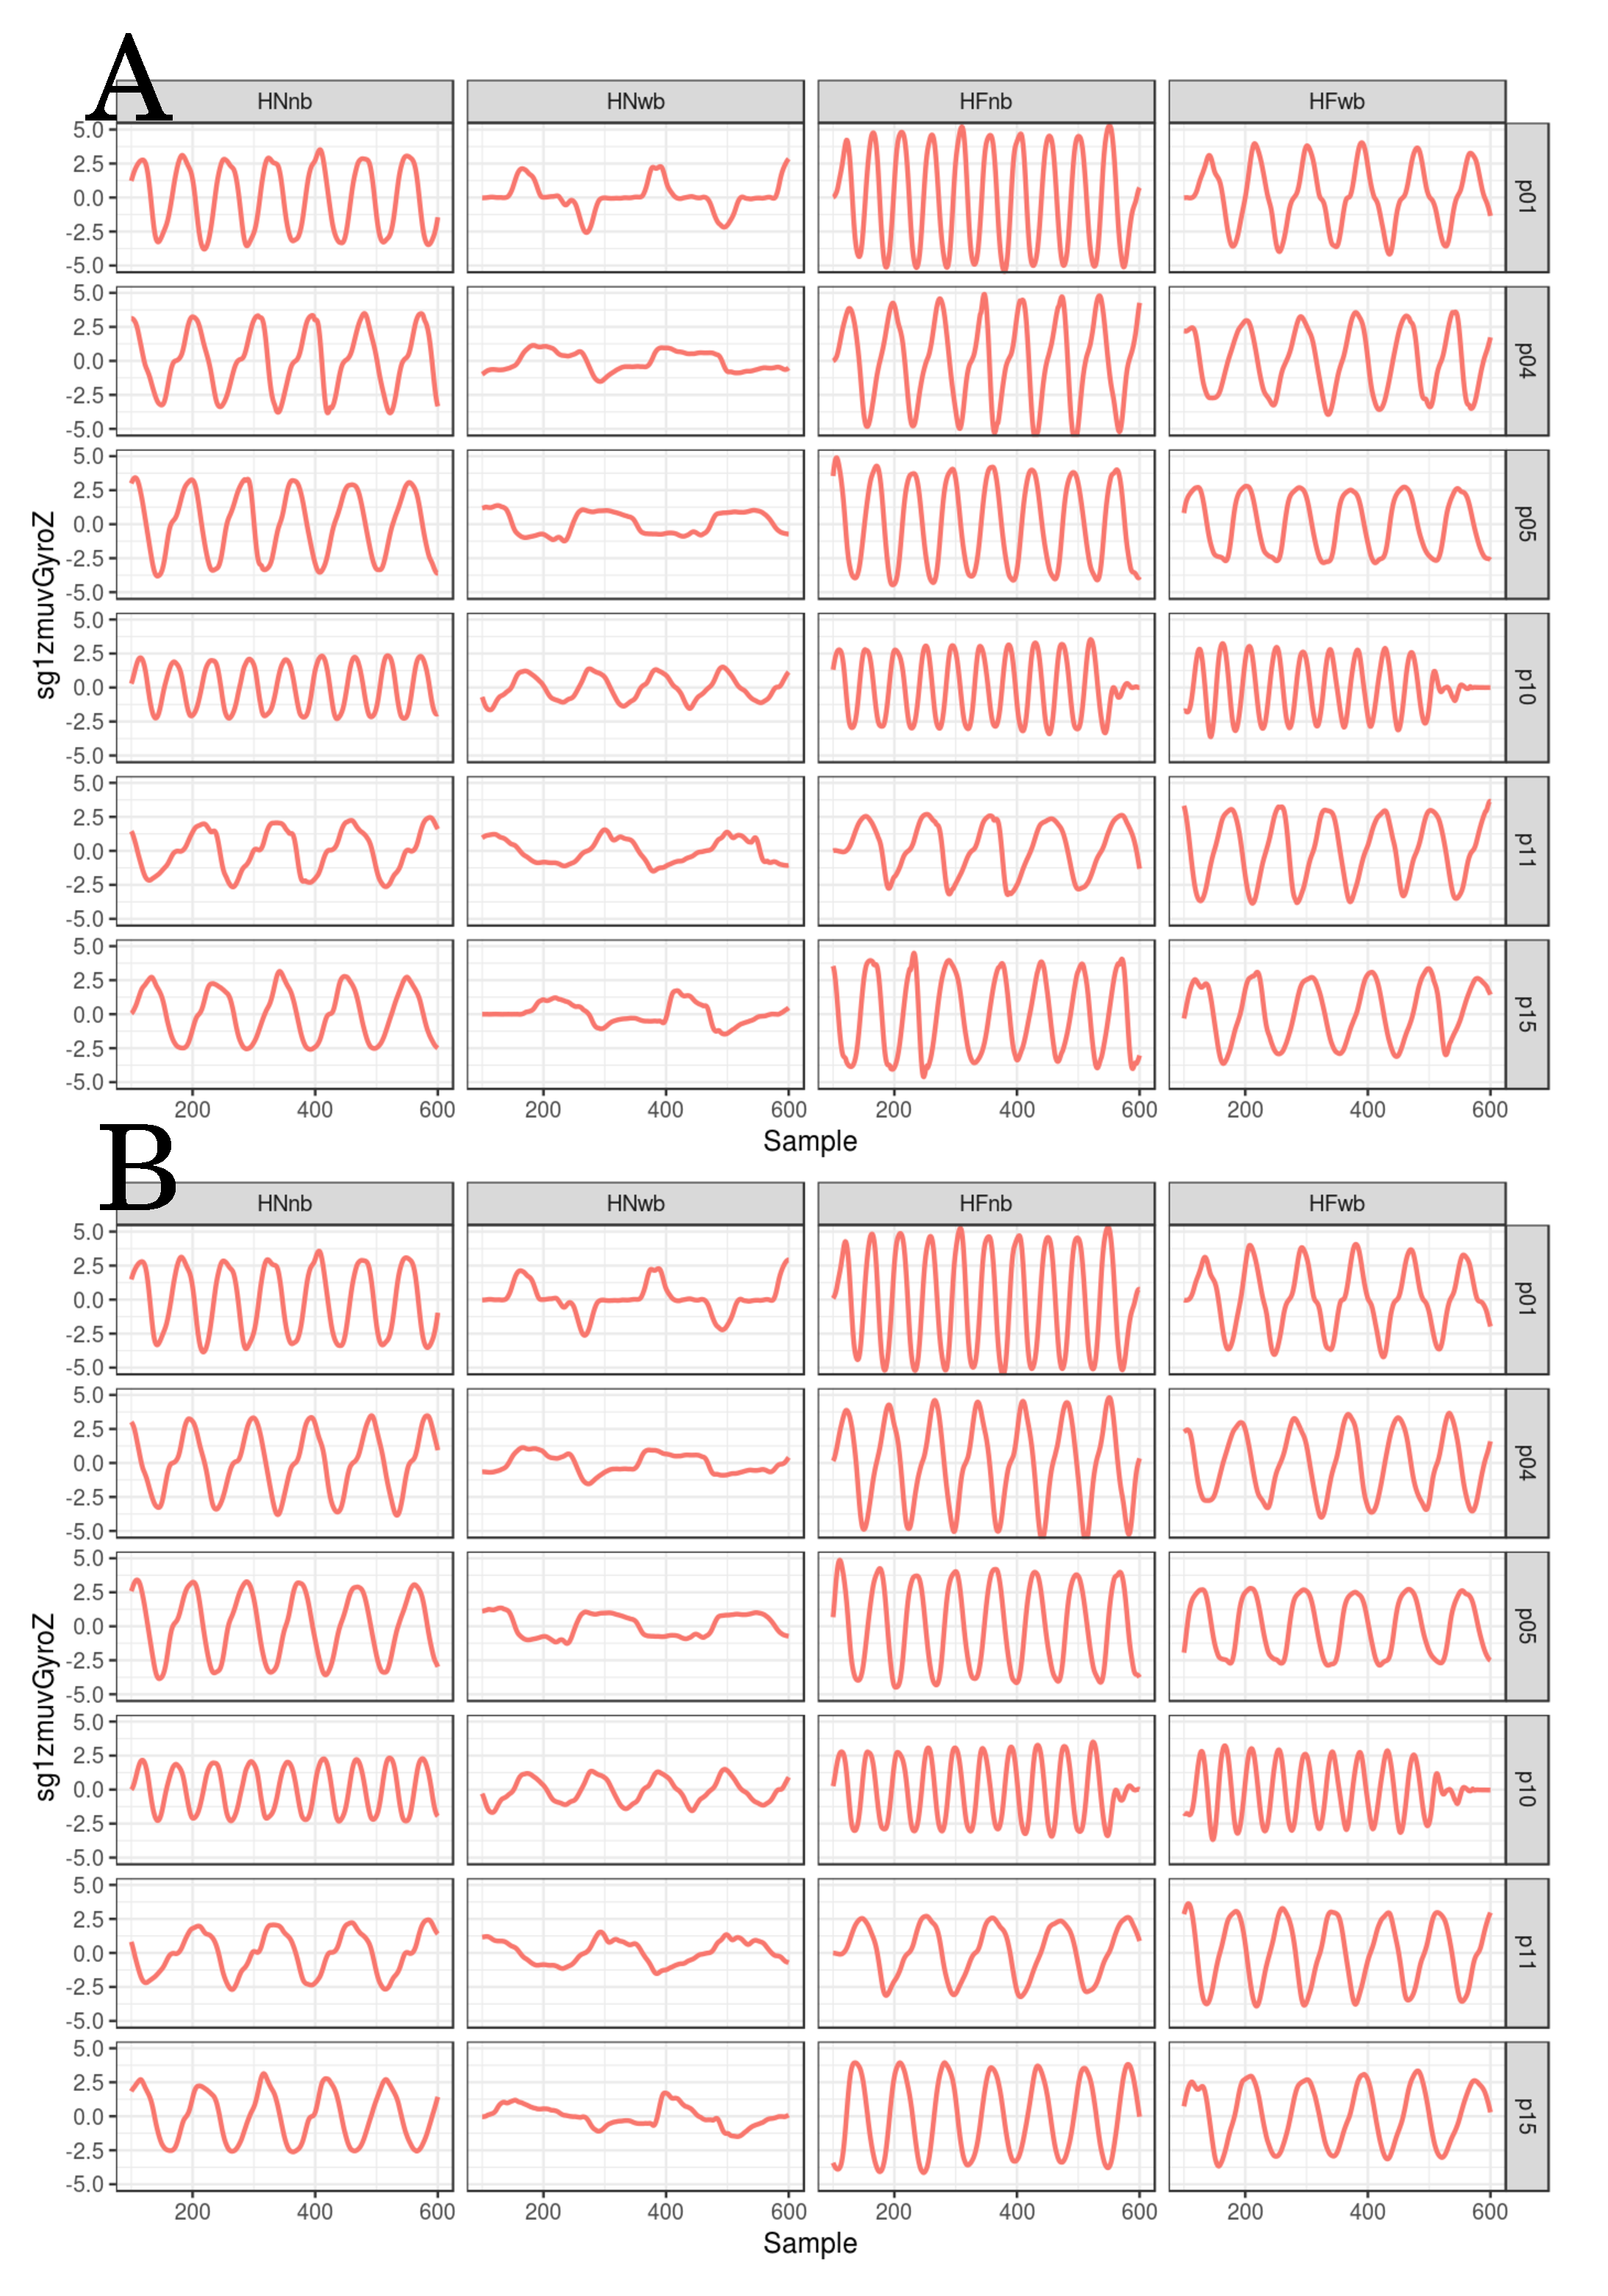
\includegraphics[width=0.8\textwidth]{tssg1gyroZ}
    	\caption
	[Time series for horizontal arm movements (sg1) ]{
	{\bf Time series for horizontal arm movements (sg1)}
		Time series for sg1GyroZ for six participants 
		($p01$, $p04$, $p05$, $p10$, $p11$, $p15$) 
		for horizontal movements in normal and faster velocity with
		no beat	(HNnb, HFnb) and with beat (HNwb, HFwb) using 
		the normalised GyroZ axis (zmuvGyroZ) and 
		two sensors attached to the participant wrist (HS01, HS02).
	R code to reproduce the figure is available from \cite{hwum2018}.
        }
    \label{fig:tssg1gyroZ-hii}
\end{figure}
%%---------------------------------(FIGURE)-----------------------------------


%%---------------------------------(FIGURE)-------------------------------------
\begin{figure}
\centering
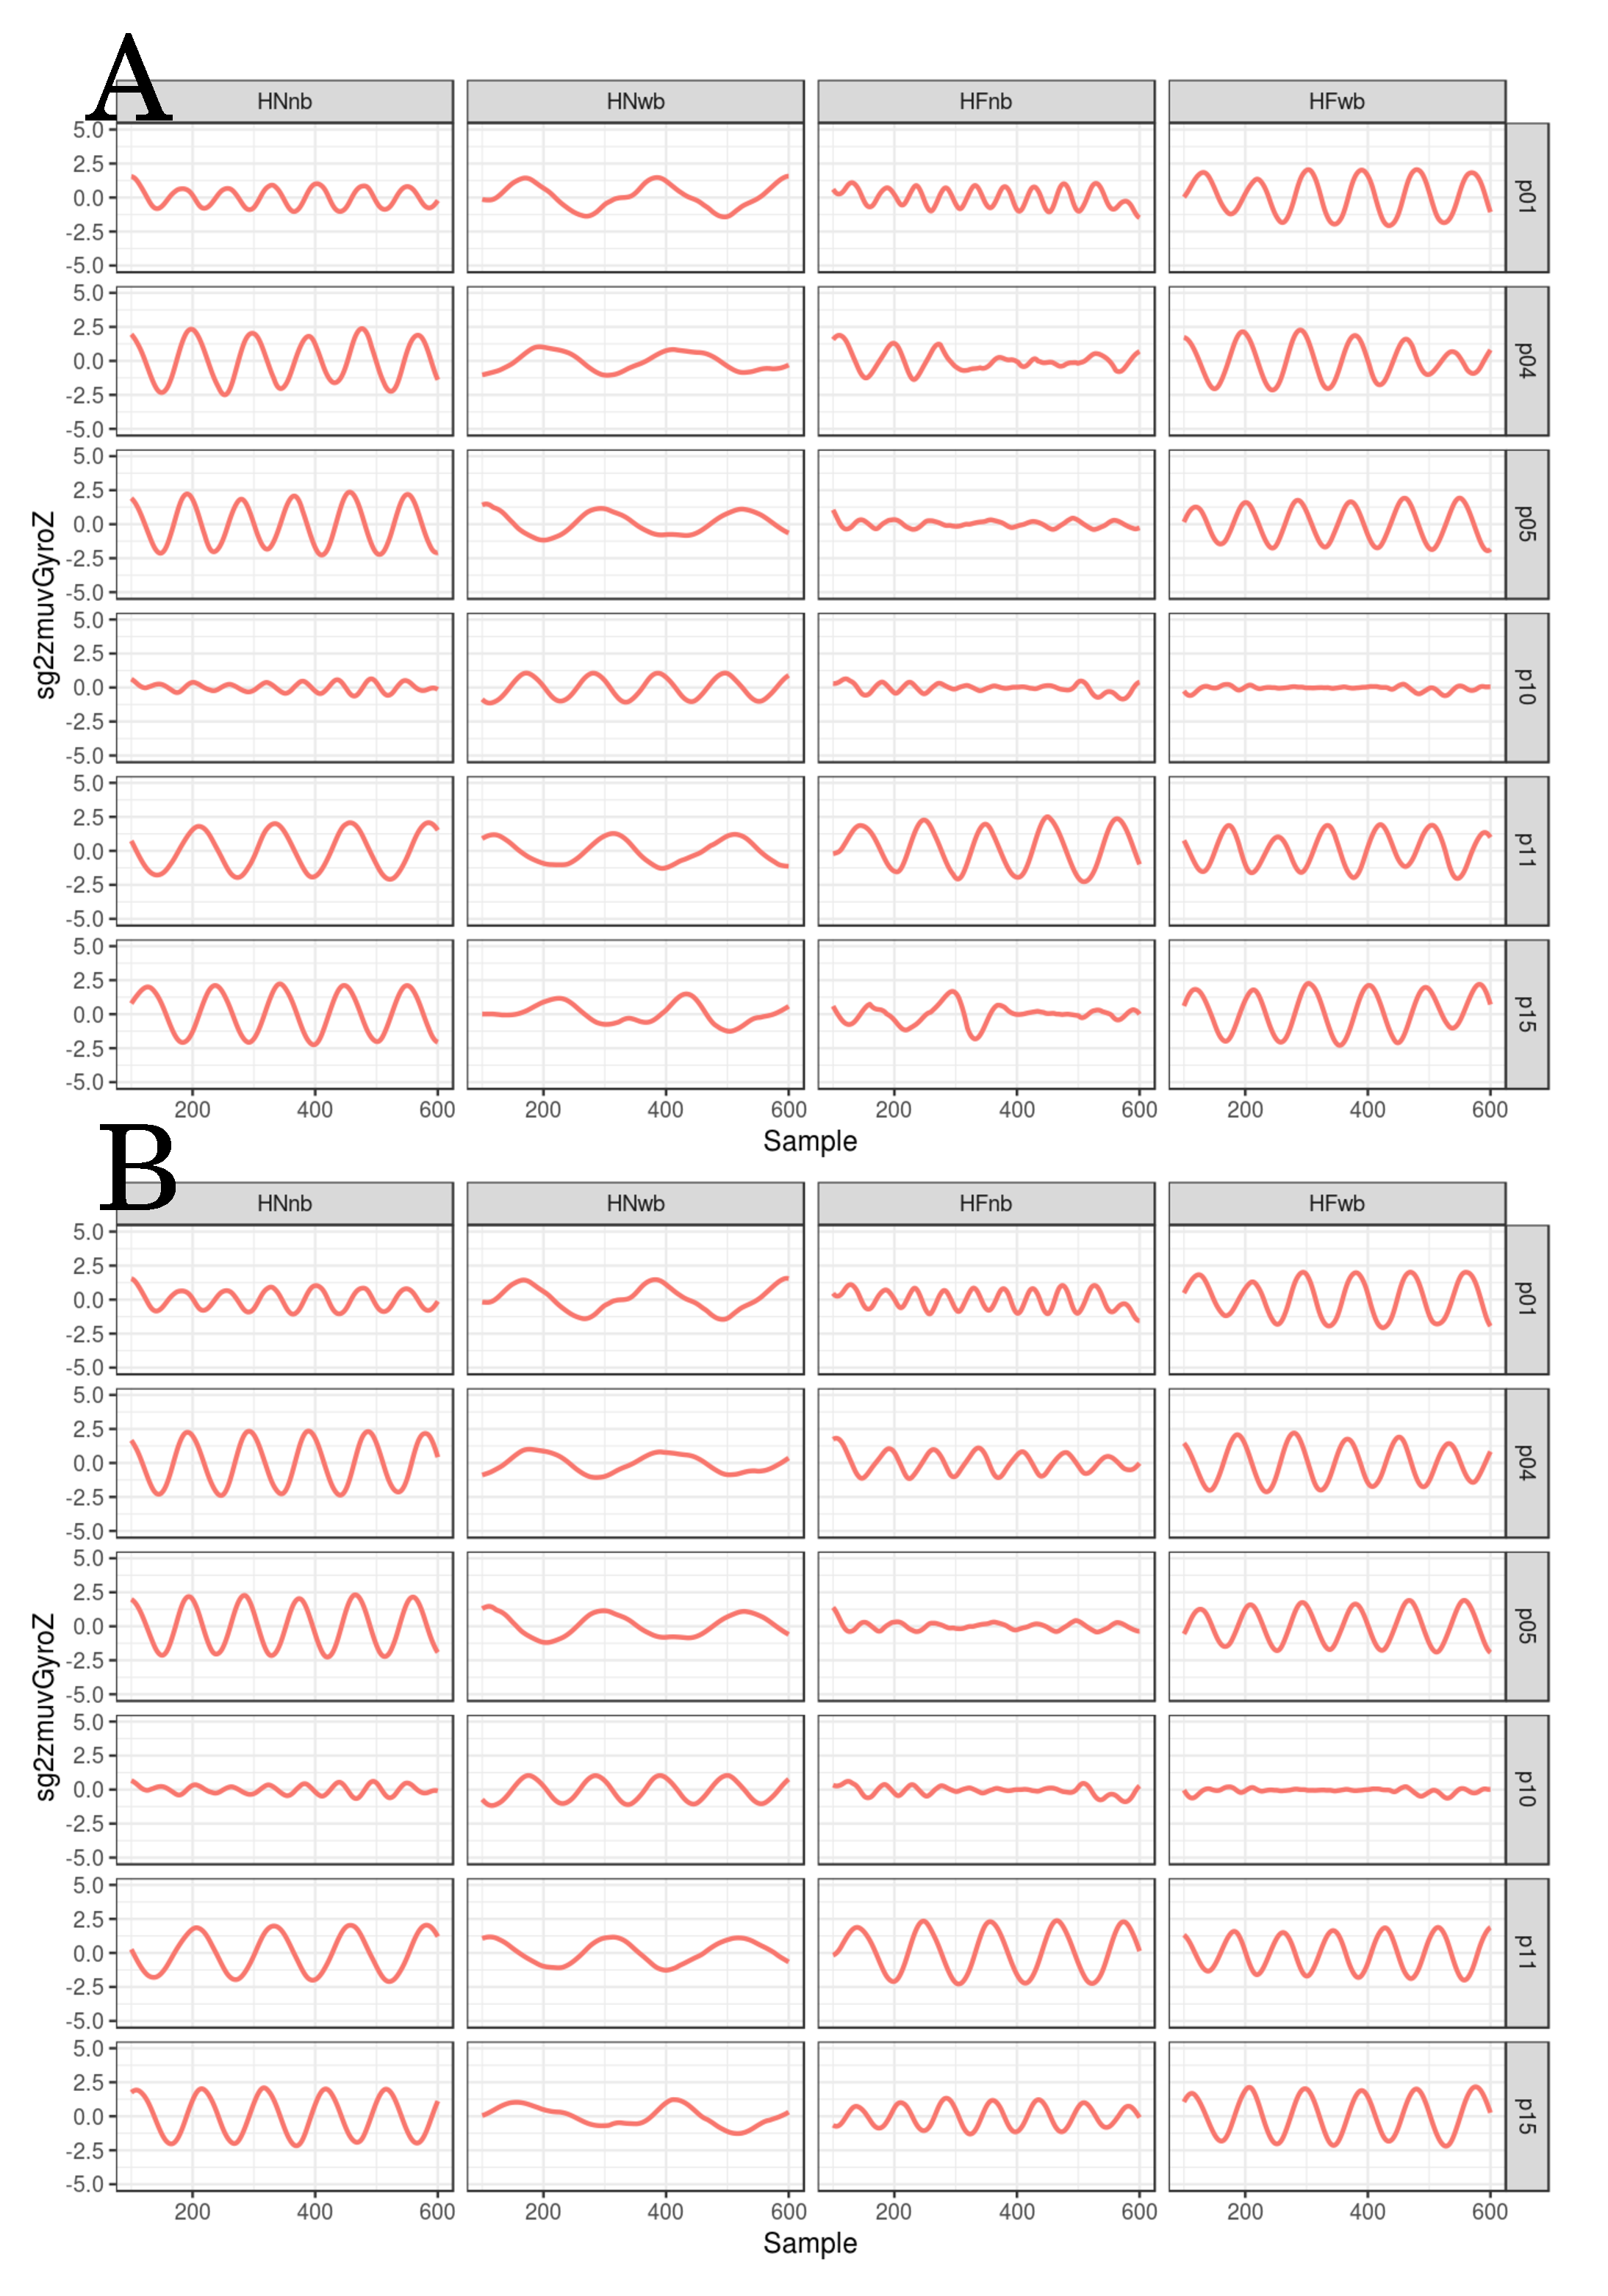
\includegraphics[width=0.8\textwidth]{tssg2gyroZ}
    	\caption
	[Time series for horizontal arm movements (sg2) ]{
	{\bf Time series for horizontal arm movements (sg2)}
		Time series for sg2GyroZ for six participants 
		($p01$, $p04$, $p05$, $p10$, $p11$, $p15$) 
		for horizontal movements in normal and faster velocity with
		no beat	(HNnb, HFnb) and with beat (HNwb, HFwb) using 
		the normalised GyroZ axis (zmuvGyroZ) and 
		two sensors attached to the participant wrist (HS01, HS02).
	R code to reproduce the figure is available from \cite{hwum2018}.
        }
    \label{fig:tssg2gyroZ-hii}
\end{figure}
%%---------------------------------(FIGURE)-----------------------------------




%%---------------------------------(FIGURE)-------------------------------------
\begin{figure}
\centering
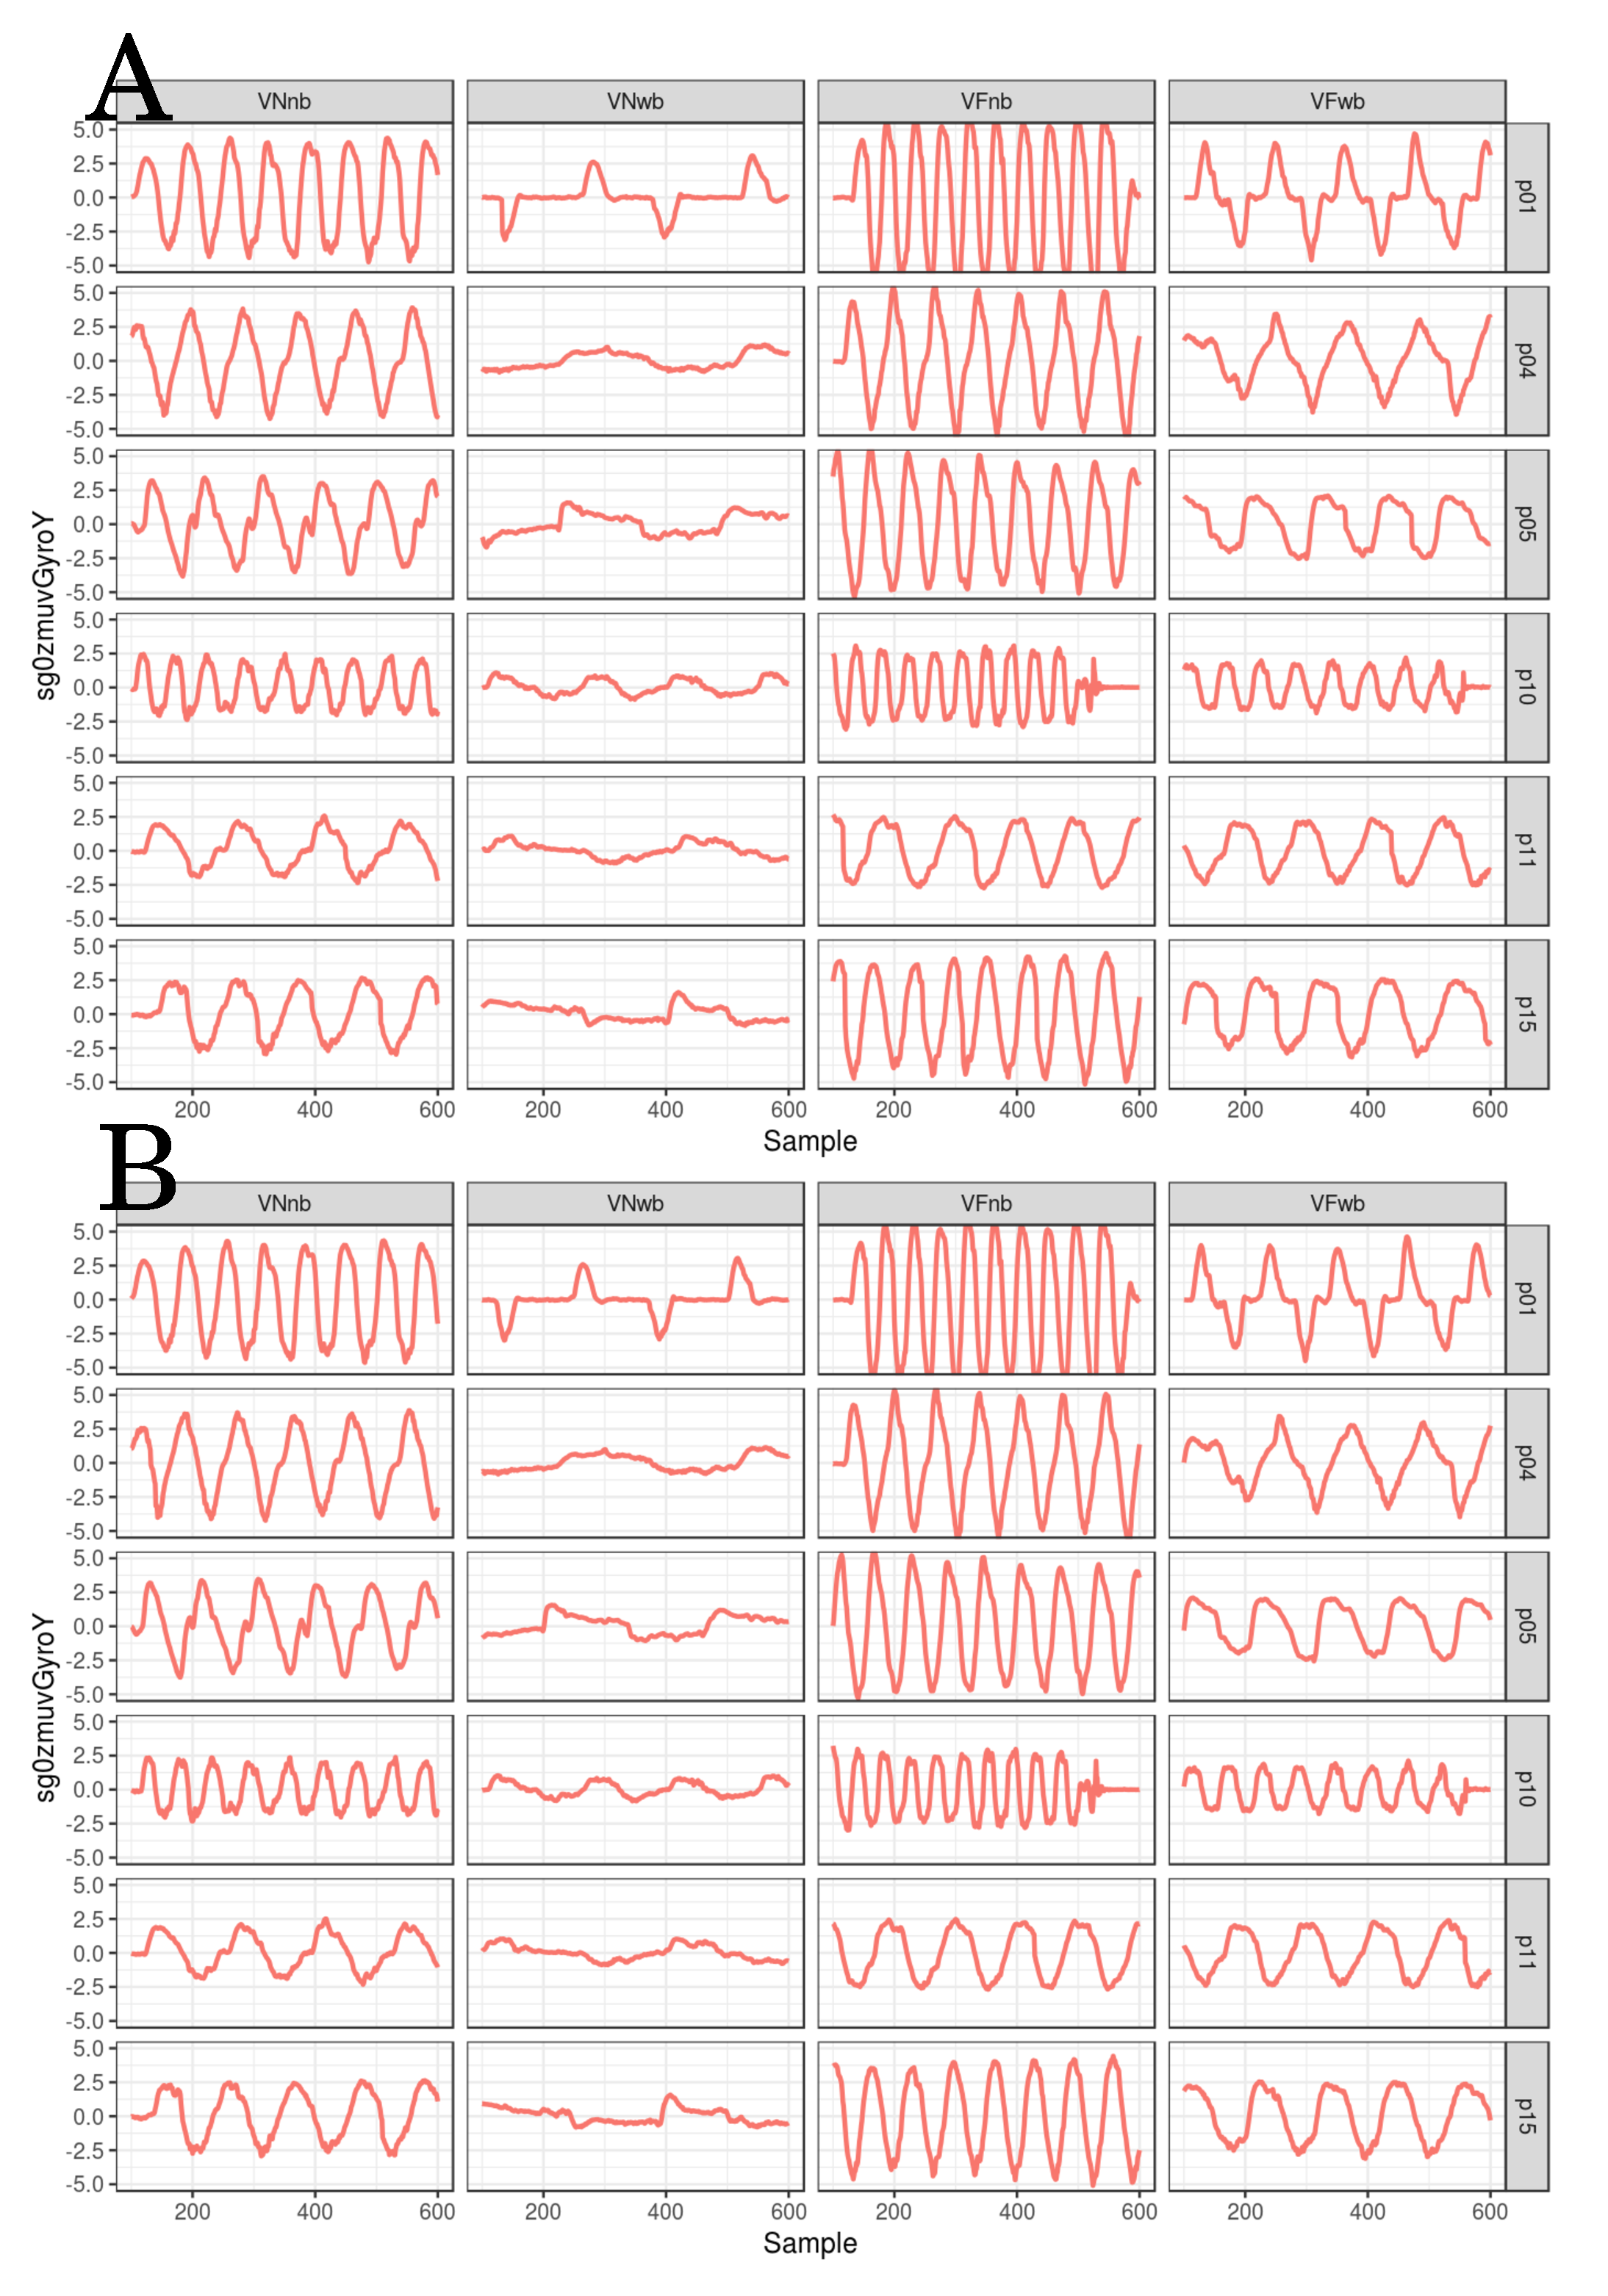
\includegraphics[width=0.8\textwidth]{tssg0gyroY}
	\caption
	[Time series for vertical arm movements (sg0) ]{
	{\bf Time series for vertical arm movements (sg0)}
		Time series for sg0GyroY  are for six participants 
		($p01$, $p04$, $p05$, $p10$, $p11$, $p15$) 
		for vertical movements in normal and faster velocity with
		no beat	(VNnb, VFnb) and with beat (VNwb, VFwb) using 
		the normalised GyroZ axis (zmuvGyroY) and 
		two sensors attached to the participant wrist (HS01, HS02).
	R code to reproduce the figure is available from \cite{hwum2018}.
	}
    \label{fig:tssg0gyroY-hii}
\end{figure}
%%---------------------------------(FIGURE)-----------------------------------


%%---------------------------------(FIGURE)-------------------------------------
\begin{figure}
\centering
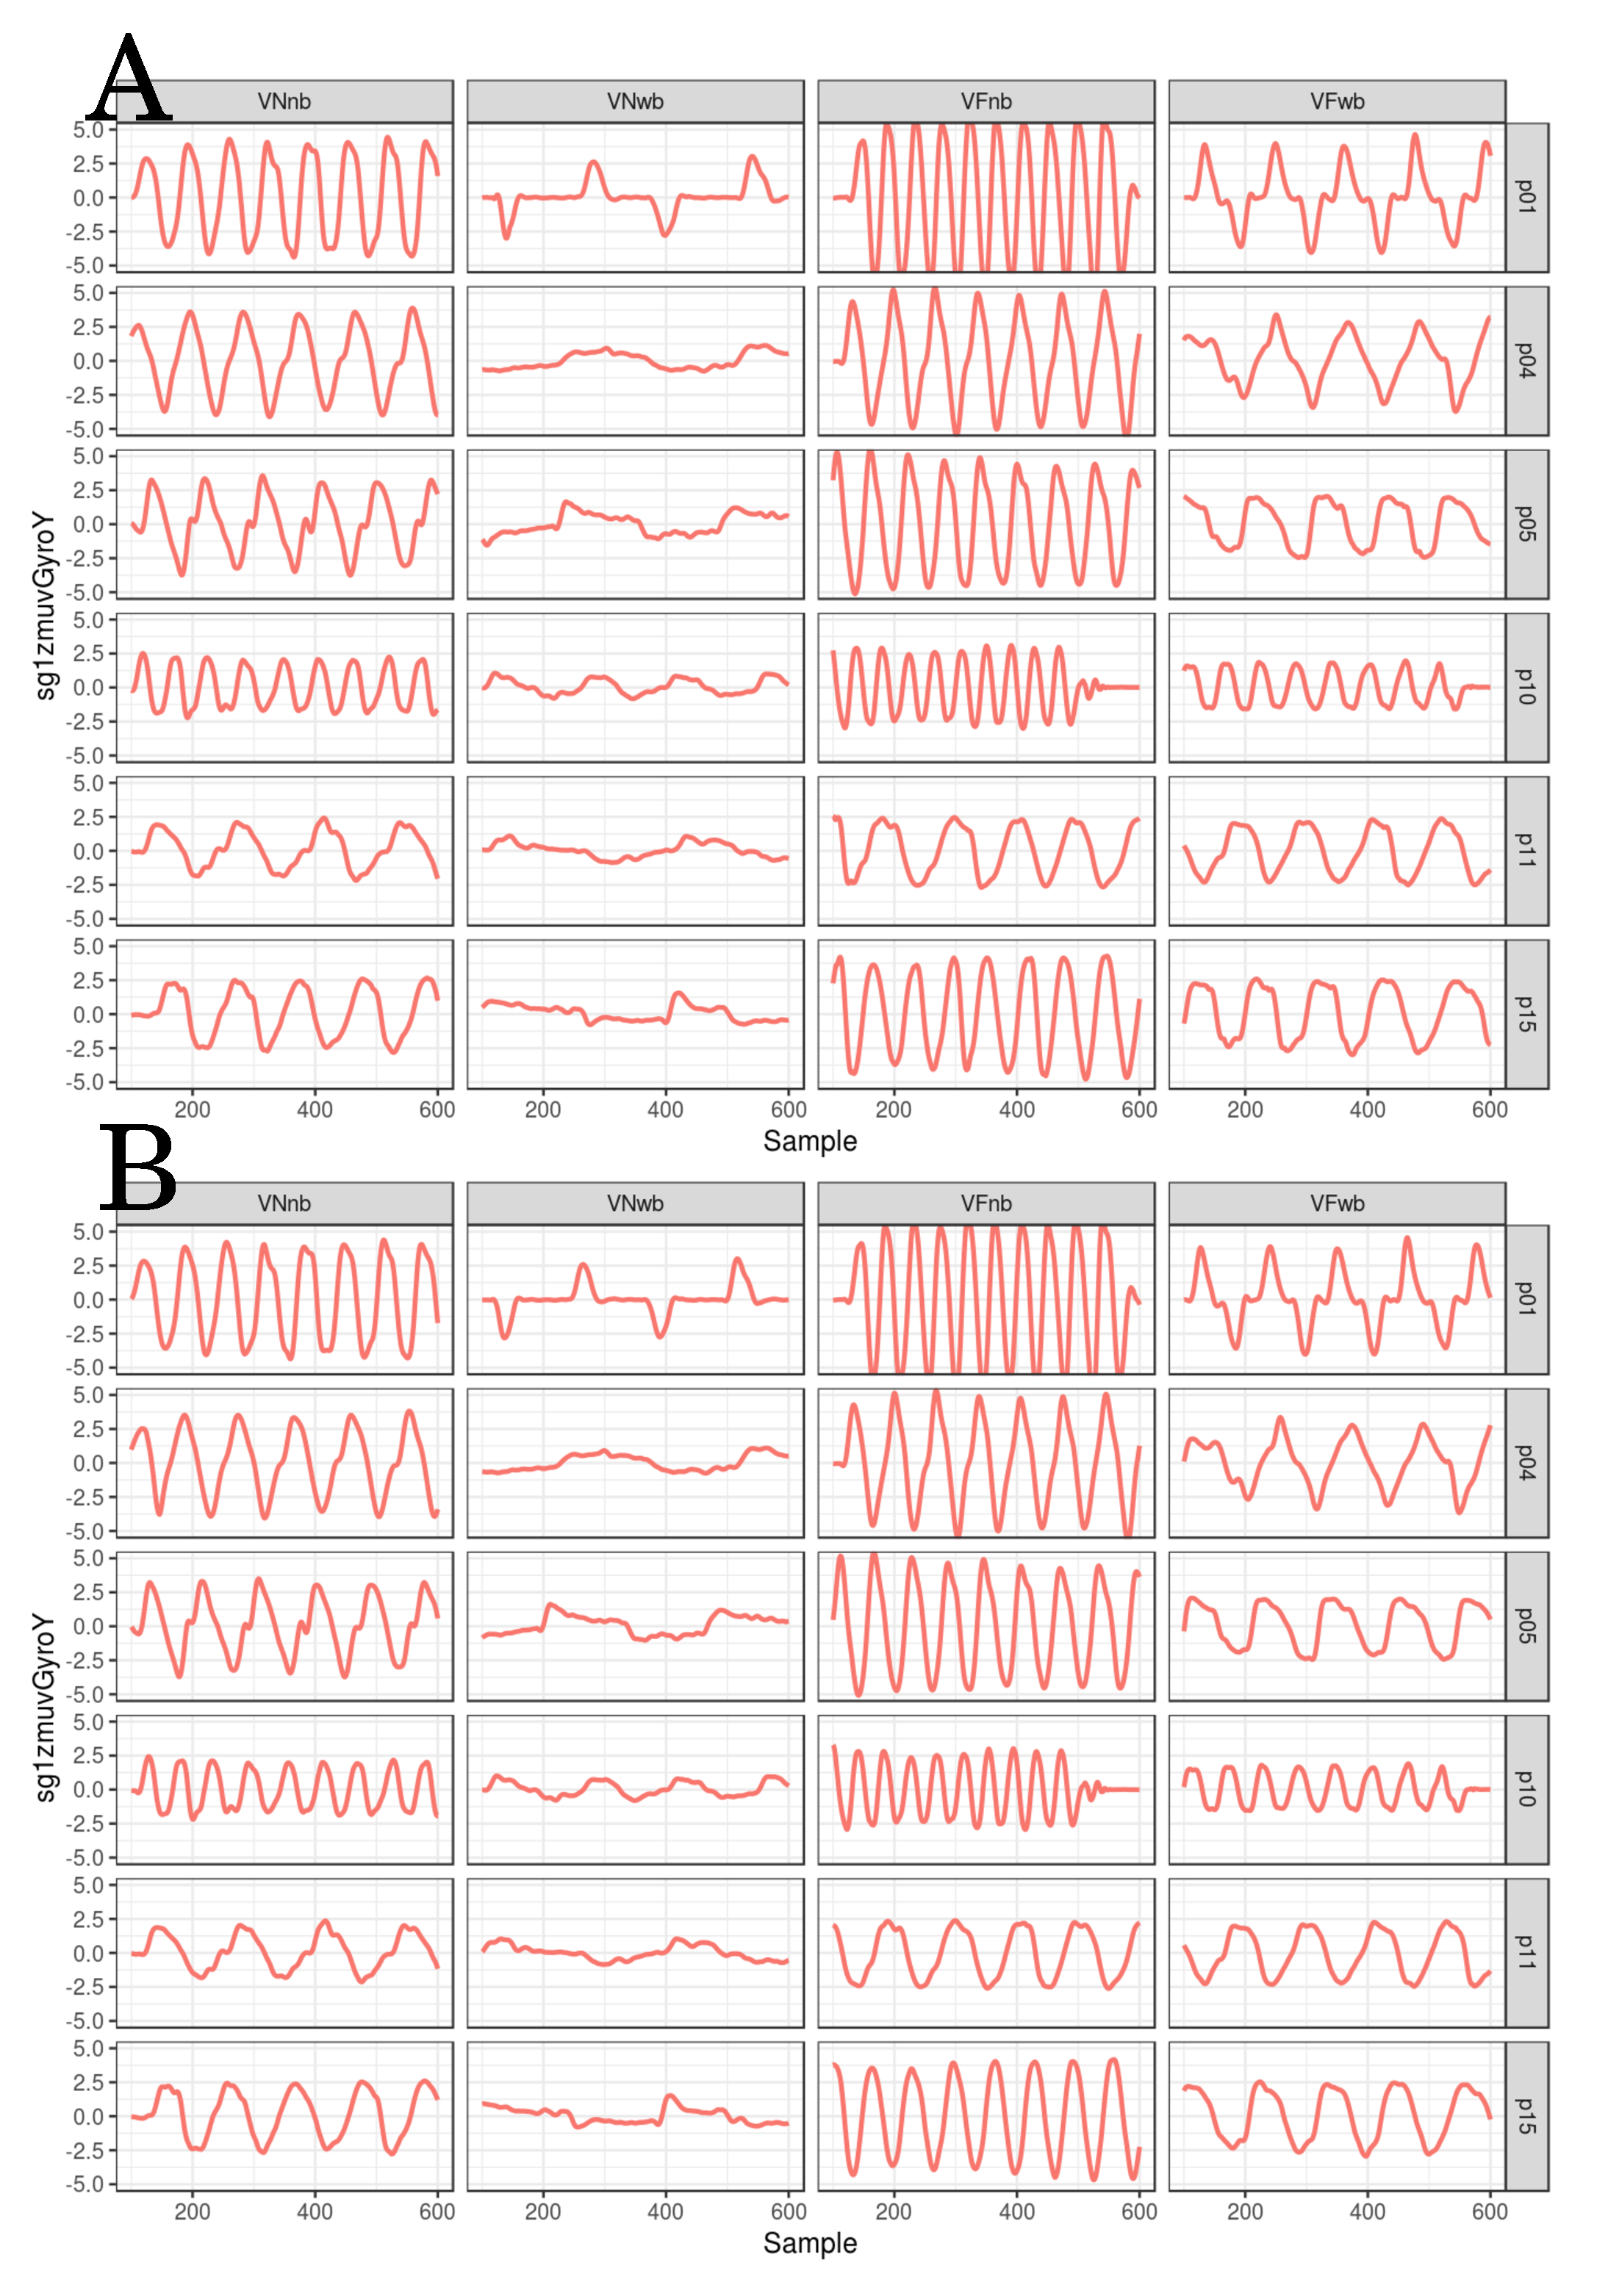
\includegraphics[width=0.8\textwidth]{tssg1gyroY}
	\caption
	[Time series for vertical arm movements (sg1) ]{
	{\bf Time series for vertical arm movements (sg1)}
		Time series for sg1GyroY for six participants 
		($p01$, $p04$, $p05$, $p10$, $p11$, $p15$) 
		for vertical movements in normal and faster velocity with
		no beat	(VNnb, VFnb) and with beat (VNwb, VFwb) using 
		the normalised GyroZ axis (zmuvGyroY) and 
		two sensors attached to the participant wrist (HS01, HS02).
	R code to reproduce the figure is available from \cite{hwum2018}.
	}
    \label{fig:tssg1gyroY-hii}
\end{figure}
%%---------------------------------(FIGURE)-----------------------------------


%%---------------------------------(FIGURE)-------------------------------------
\begin{figure}
\centering
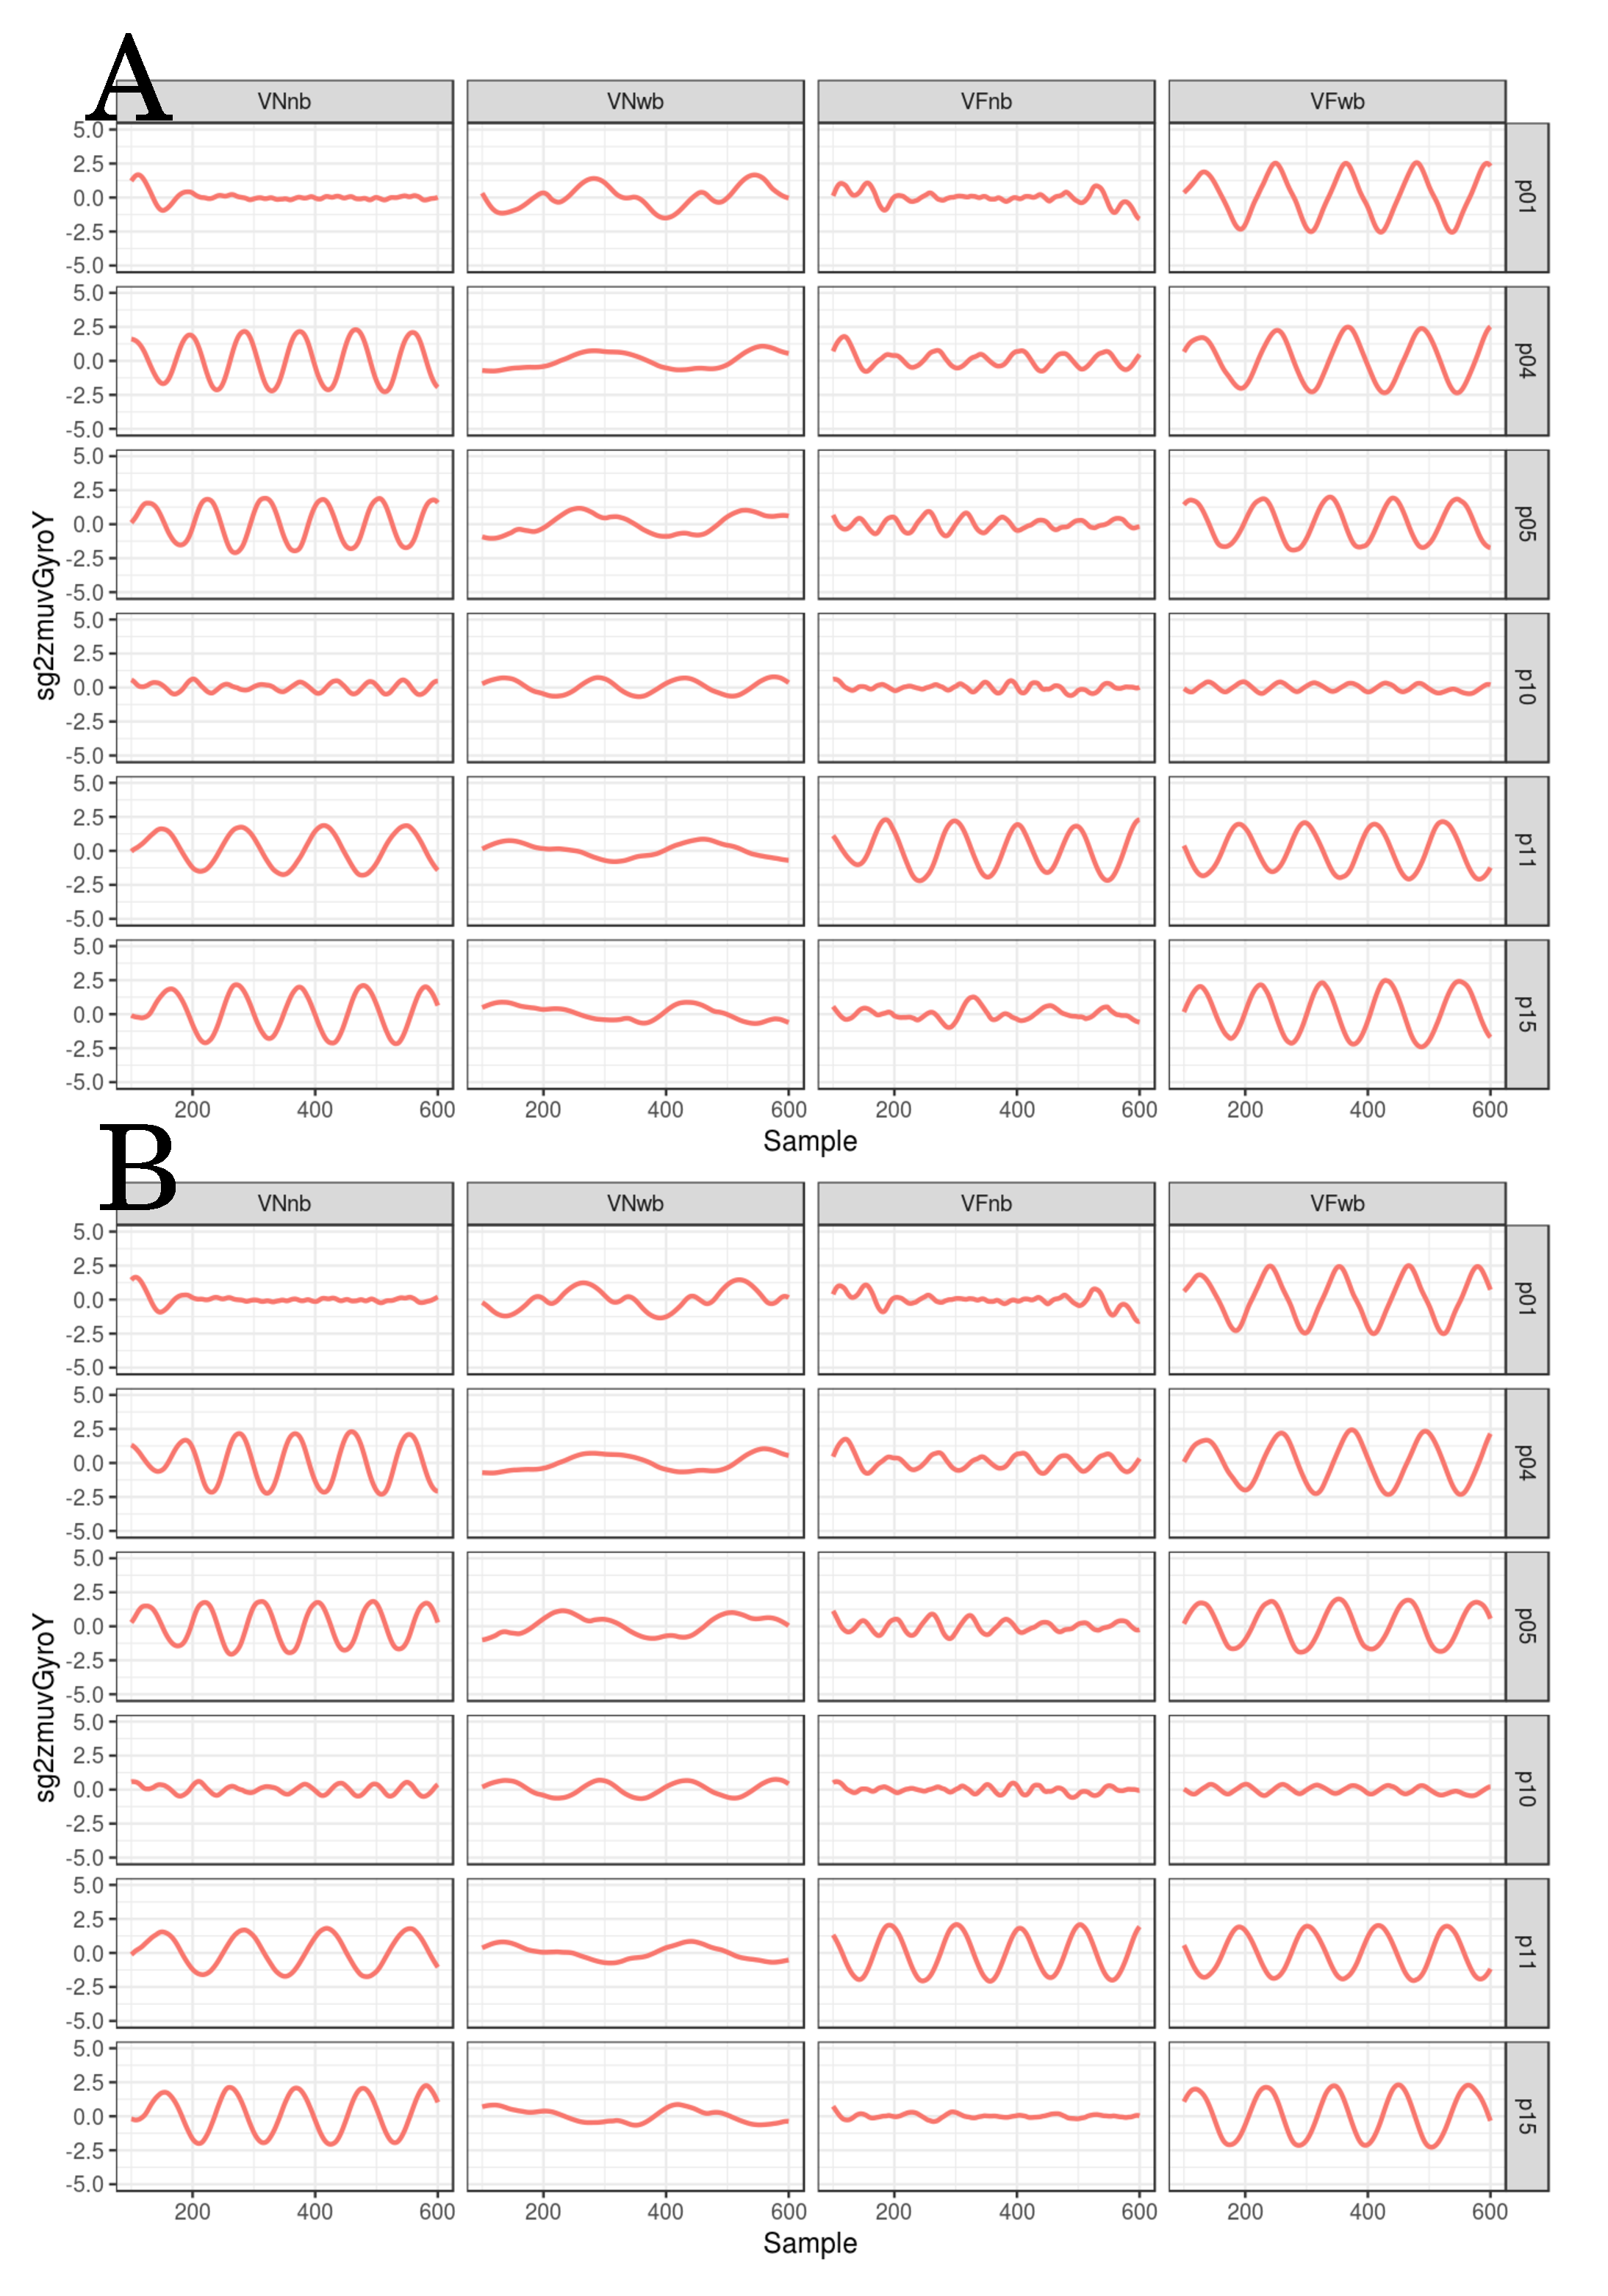
\includegraphics[width=0.8\textwidth]{tssg2gyroY}
	\caption
	[Time series for vertical arm movements (sg2) ]{
	{\bf Time series for vertical arm movements (sg2)}
		Time series for sg2GyroY for six participants 
		($p01$, $p04$, $p05$, $p10$, $p11$, $p15$) 
		for vertical movements in normal and faster velocity with
		no beat	(VNnb, VFnb) and with beat (VNwb, VFwb) using 
		the normalised GyroY axis (zmuvGyroY) and 
		two sensors attached to the participant wrist (HS01, HS02).
	R code to reproduce the figure is available from \cite{hwum2018}.
	}
    \label{fig:tssg2gyroY-hii}
\end{figure}
%%---------------------------------(FIGURE)-----------------------------------







\newpage
\section{Embedding parameters} \label{appendix:d:ep}
\subsection{Minimum dimension embedding values}
Values of minimum embedding dimensions for horizontal normal arm movements 
with no beat (HNnb) and horizontal faster arm movements 
with no beat (HFnb) are shown in Fig \ref{fig:caoHnb} which values of 
minimum embedding dimensions present a fluctuation of values between four 
and seven over six participants.
It can also be noted a slightly variation of minimum embedding dimension values 
over participants when comparing HS01 and HS02 (Fig \ref{fig:caoHnb}(A, B)).
With regards to the smoothness of the time series,
the minimum embedding values are also smoothed showing less variations of
values over six participants (Fig \ref{fig:caoHnb}).

Values of minimum embedding dimension for horizontal normal arm movements 
with beat (HNwb) and horizontal faster arm movements with beat (HFwb) 
are shown in Fig \ref{fig:caoHwb} where is shown a fluctuations of values
for minimum embedding dimension between five and seven.
Similarly as in Fig \ref{fig:caoHnb}, Fig \ref{fig:caoHwb} show changes of 
minimum embedding dimension between participants and the smoothness of the 
time series also affects the smoothness of minimum embedding dimension values.


Values of minimum embedding dimension for vertical arm movements with no beat
are shown in Figs \ref{fig:caoVnb}(A, B) where the smoothness 
of the time series have little effect on the minimum embedding dimension 
values, whereas smoothness of time series affects the smoothness of the 
minimum embedding values for vertical faster arm movements with no beats 
(Fig \ref{fig:caoVnb}(C, D)).

Fig \ref{fig:caoVwb} shows the variation of minimum embedding values for 
vertical arm movements with beat where the smoothness of the time series
affects both vertical normal and vertical faster movements with a slight 
decrease on each of the values as the smoothness increase.




%Horizontal arm movements
%%---------------------------------(FIGURE)-------------------------------------
\begin{figure}
\centering
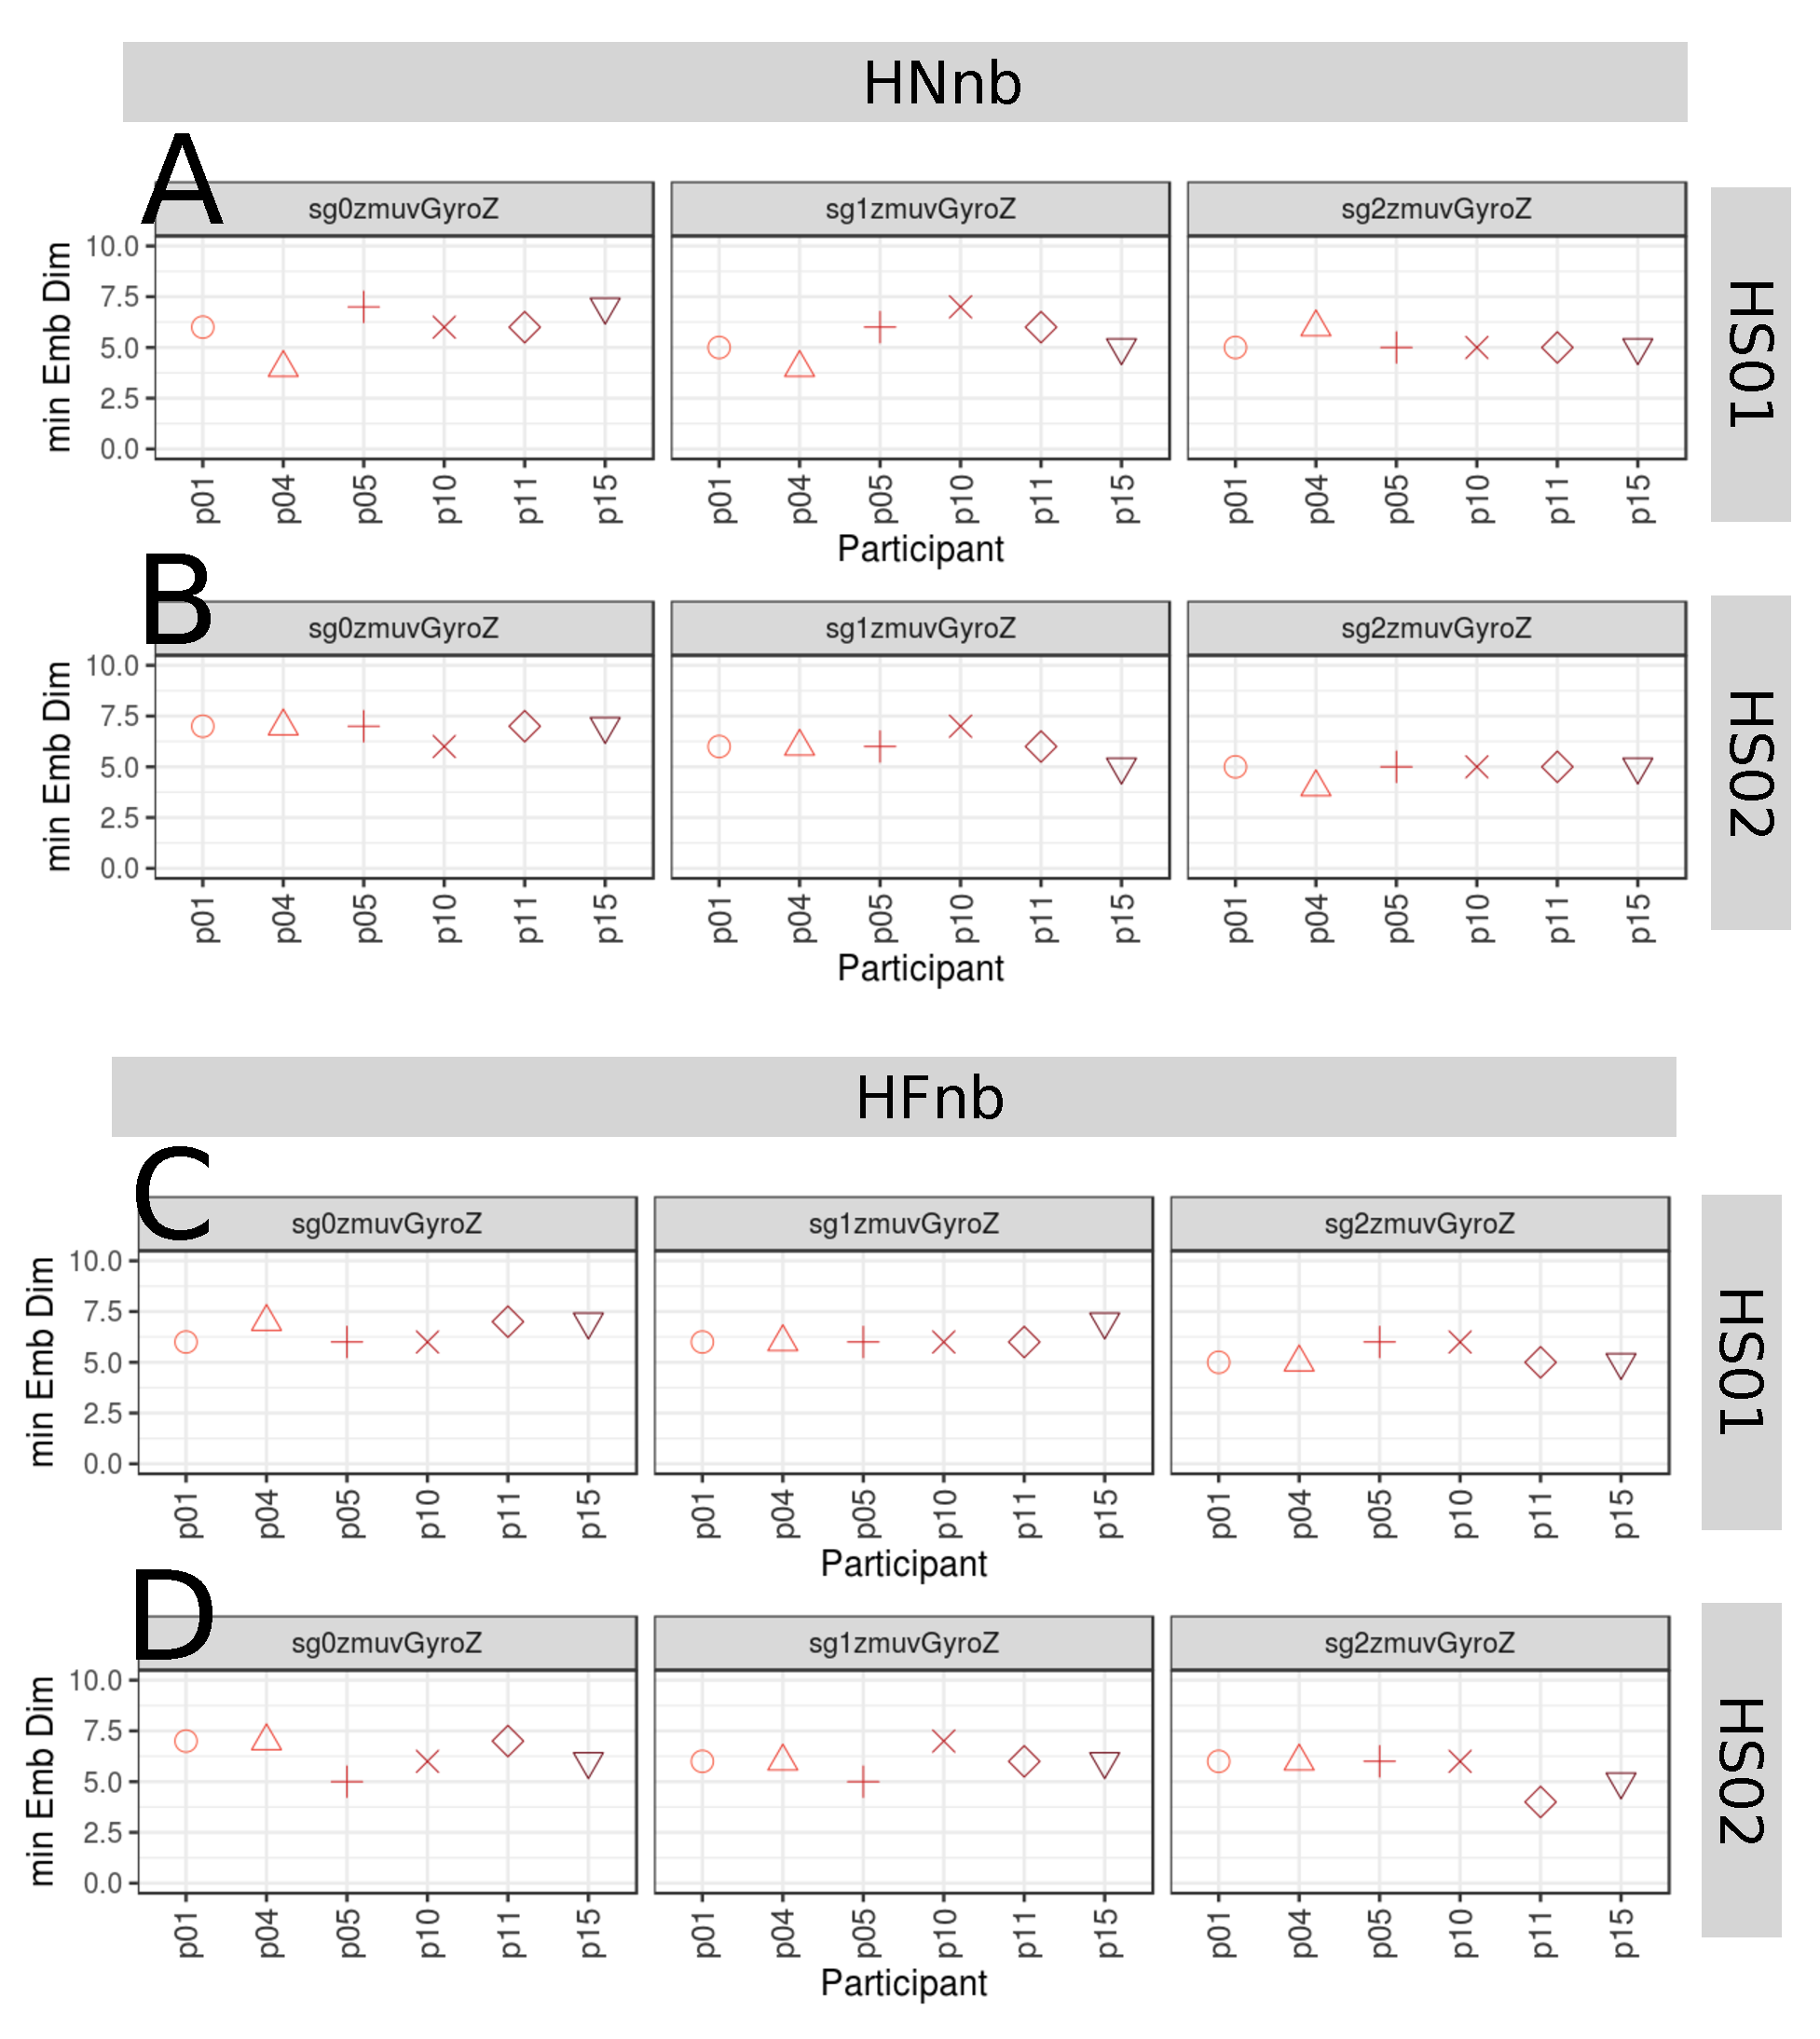
\includegraphics[width=1.0\textwidth]{cao_Hnb_w10}
	\caption
	[Minimum embedding dimensions for horizontal arm movements 
	(no beat)]{
	{\bf Minimum embedding dimensions for horizontal arm movements 
	(no beat).} 
		(A, B) Horizontal Normal with no beat (HNnb), and 
		(C, D) Horizontal Faster with no beat (HFnb) movements.
		(A, C) Sensor 01 attached to the participant (HS01), and
		(B, D) sensor 02 attached to the participant (HS02).
		Minimum embedding dimensions are for six participants 
		(p01, p04, p05, p10, p11, p15) with three smoothed signals 
		(sg0zmuvGyroZ, sg1zmuvGyroZ and sg2zmuvGyroZ)
		and window lenght of 10-sec (500 samples).
		R code to reproduce the figure is available 
		from \cite{hwum2018}.
        }
    \label{fig:caoHnb}
\end{figure}
%%---------------------------------(FIGURE)-------------------------------------
%%---------------------------------(FIGURE)-------------------------------------
\begin{figure}
\centering
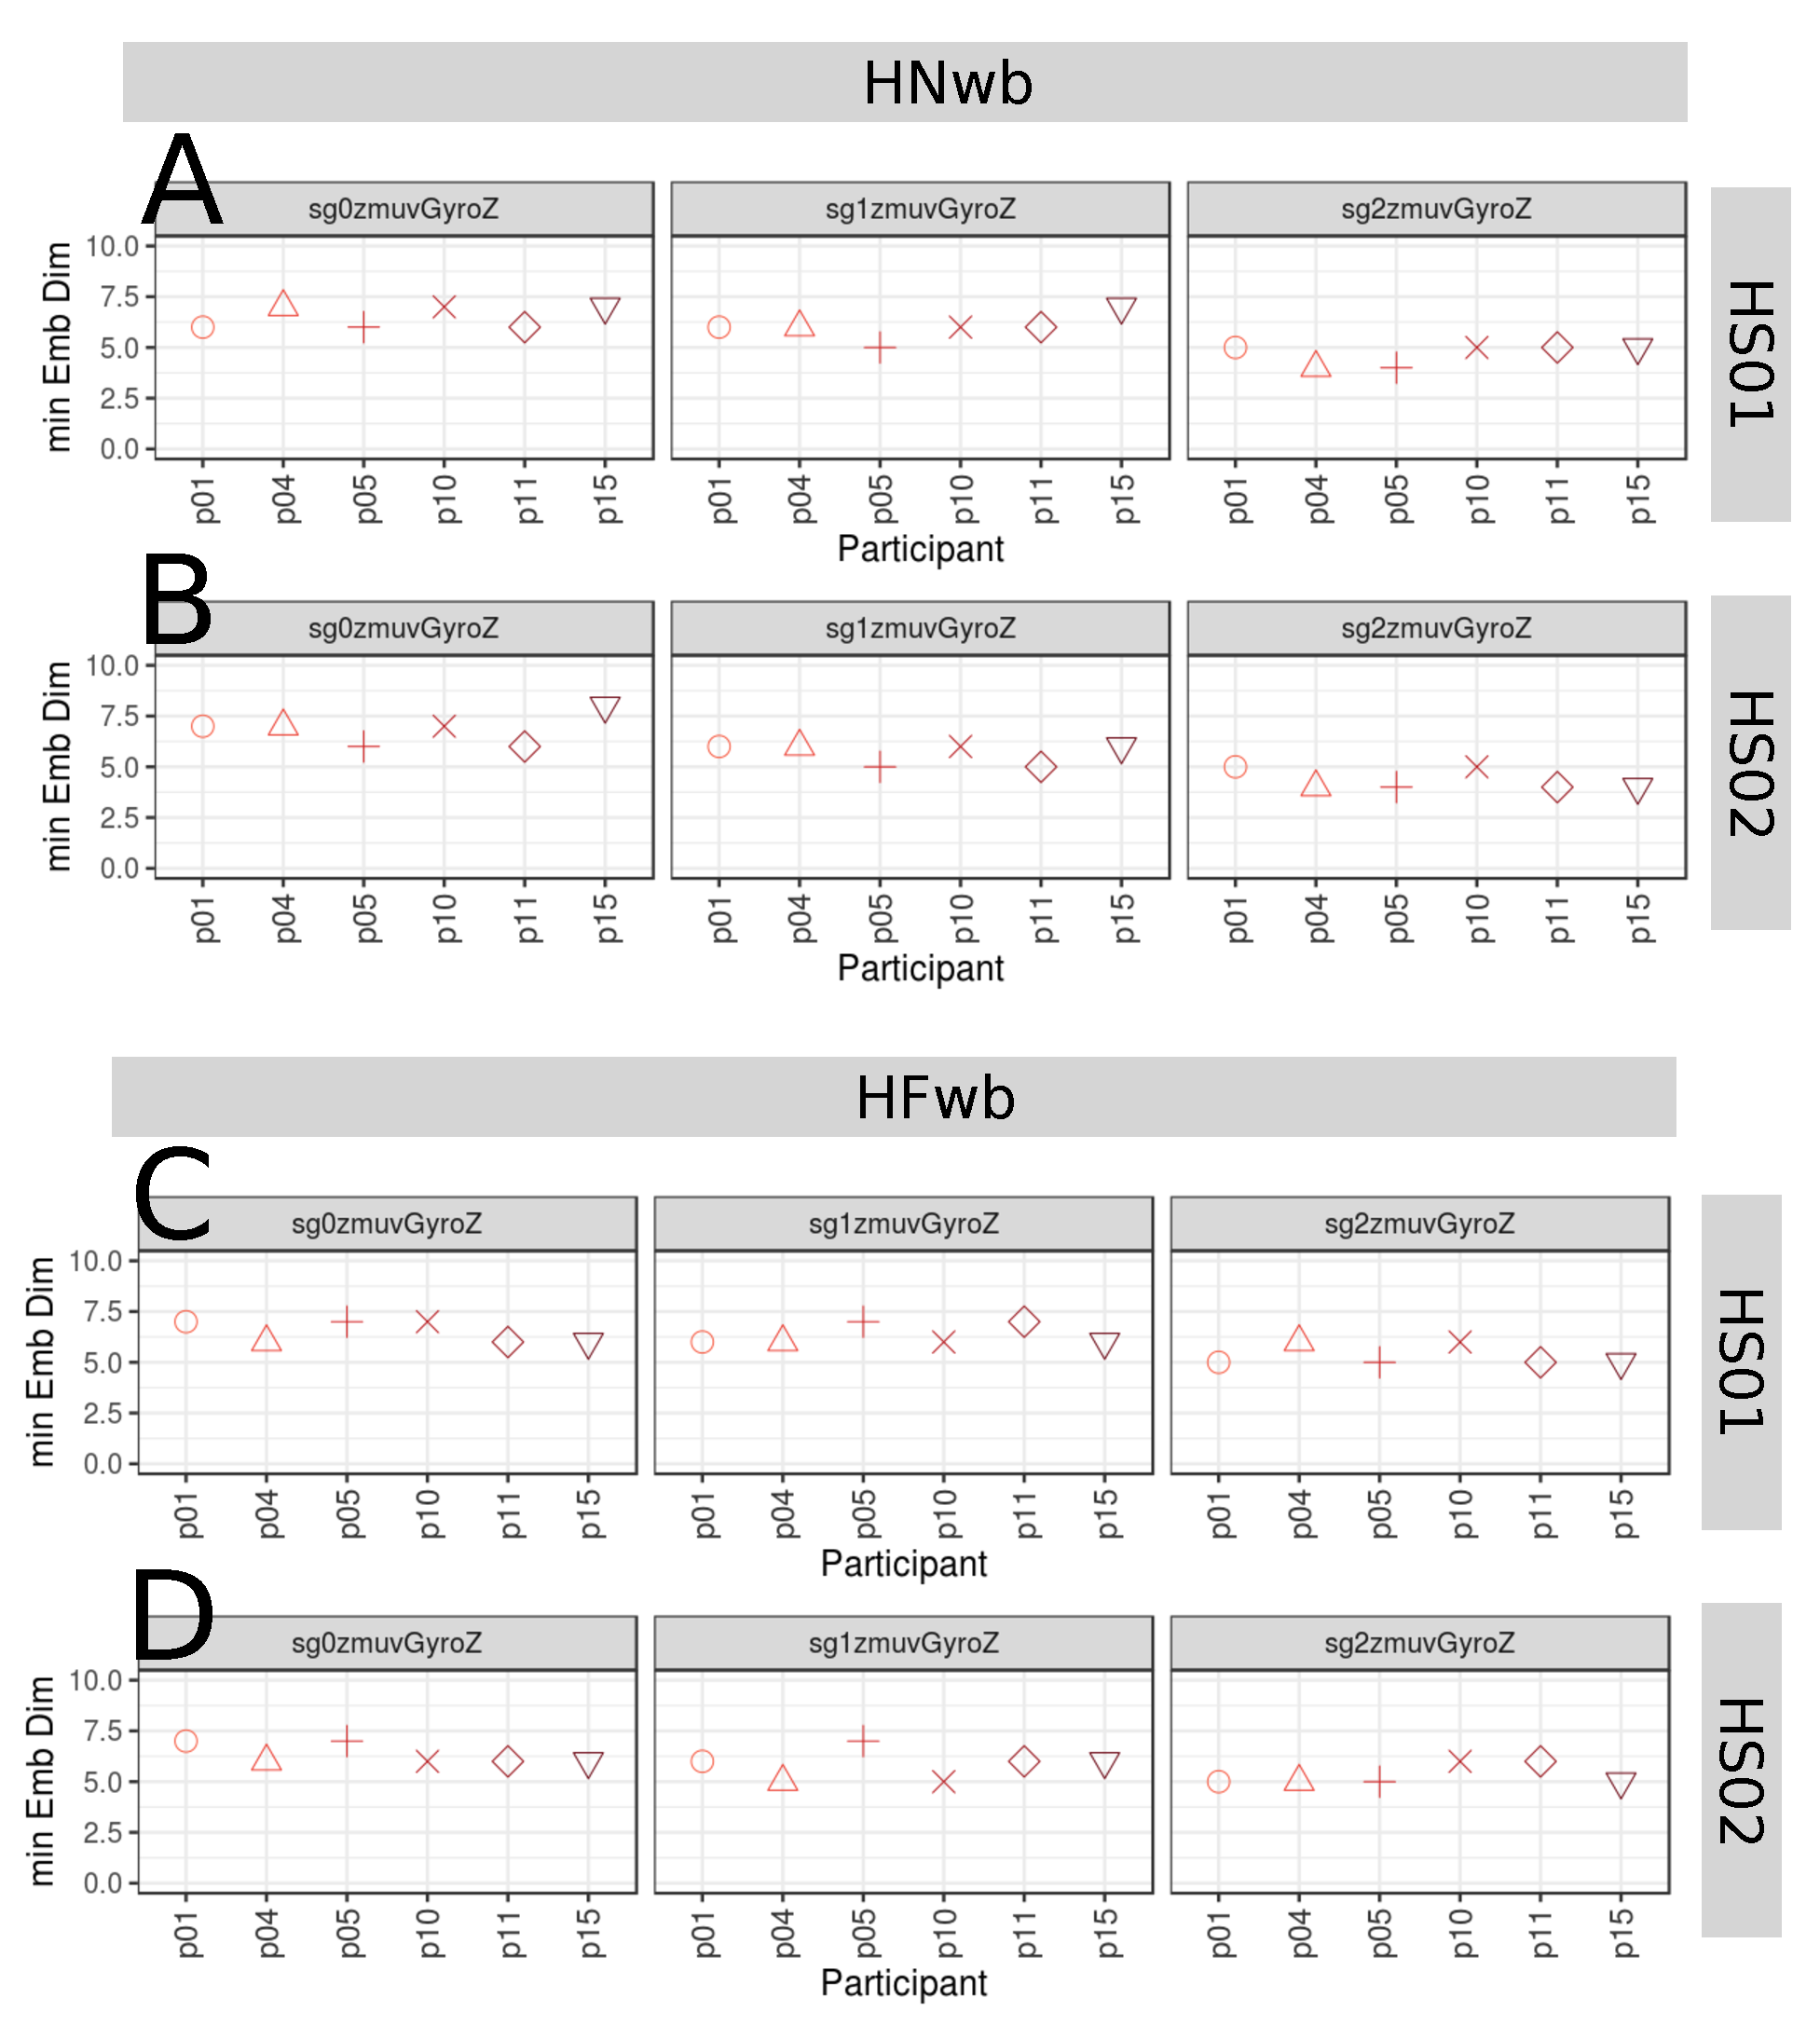
\includegraphics[width=1.0\textwidth]{cao_Hwb_w10}
	\caption
	[Minimum embedding dimensions for horizontal arm movements 
	(with beat)]{
	{\bf Minimum embedding dimensions for horizontal arm movements 
	(with beat).} 
		(A, B) Horizontal Normal with beat (HNwb), and
		(C, D) Horizontal Faster with beat (HFwb) movements.
		(A, C) Sensor 01 attached to the participant (HS01), and
		(B, D) sensor 02 attached to the participant (HS02).
		Minimum embedding dimensions are for six participants 
		(p01, p04, p05, p10, p11, p15) with three smoothed signals 
		(sg0zmuvGyroZ, sg1zmuvGyroZ and sg2zmuvGyroZ)
		and window lenght of 10-sec (500 samples).
		R code to reproduce the figure is available 
		from \cite{hwum2018}.
        }
    \label{fig:caoHwb}
\end{figure}
%%---------------------------------(FIGURE)-------------------------------------


%Vertical arm movements
%%---------------------------------(FIGURE)-------------------------------------
\begin{figure}
\centering
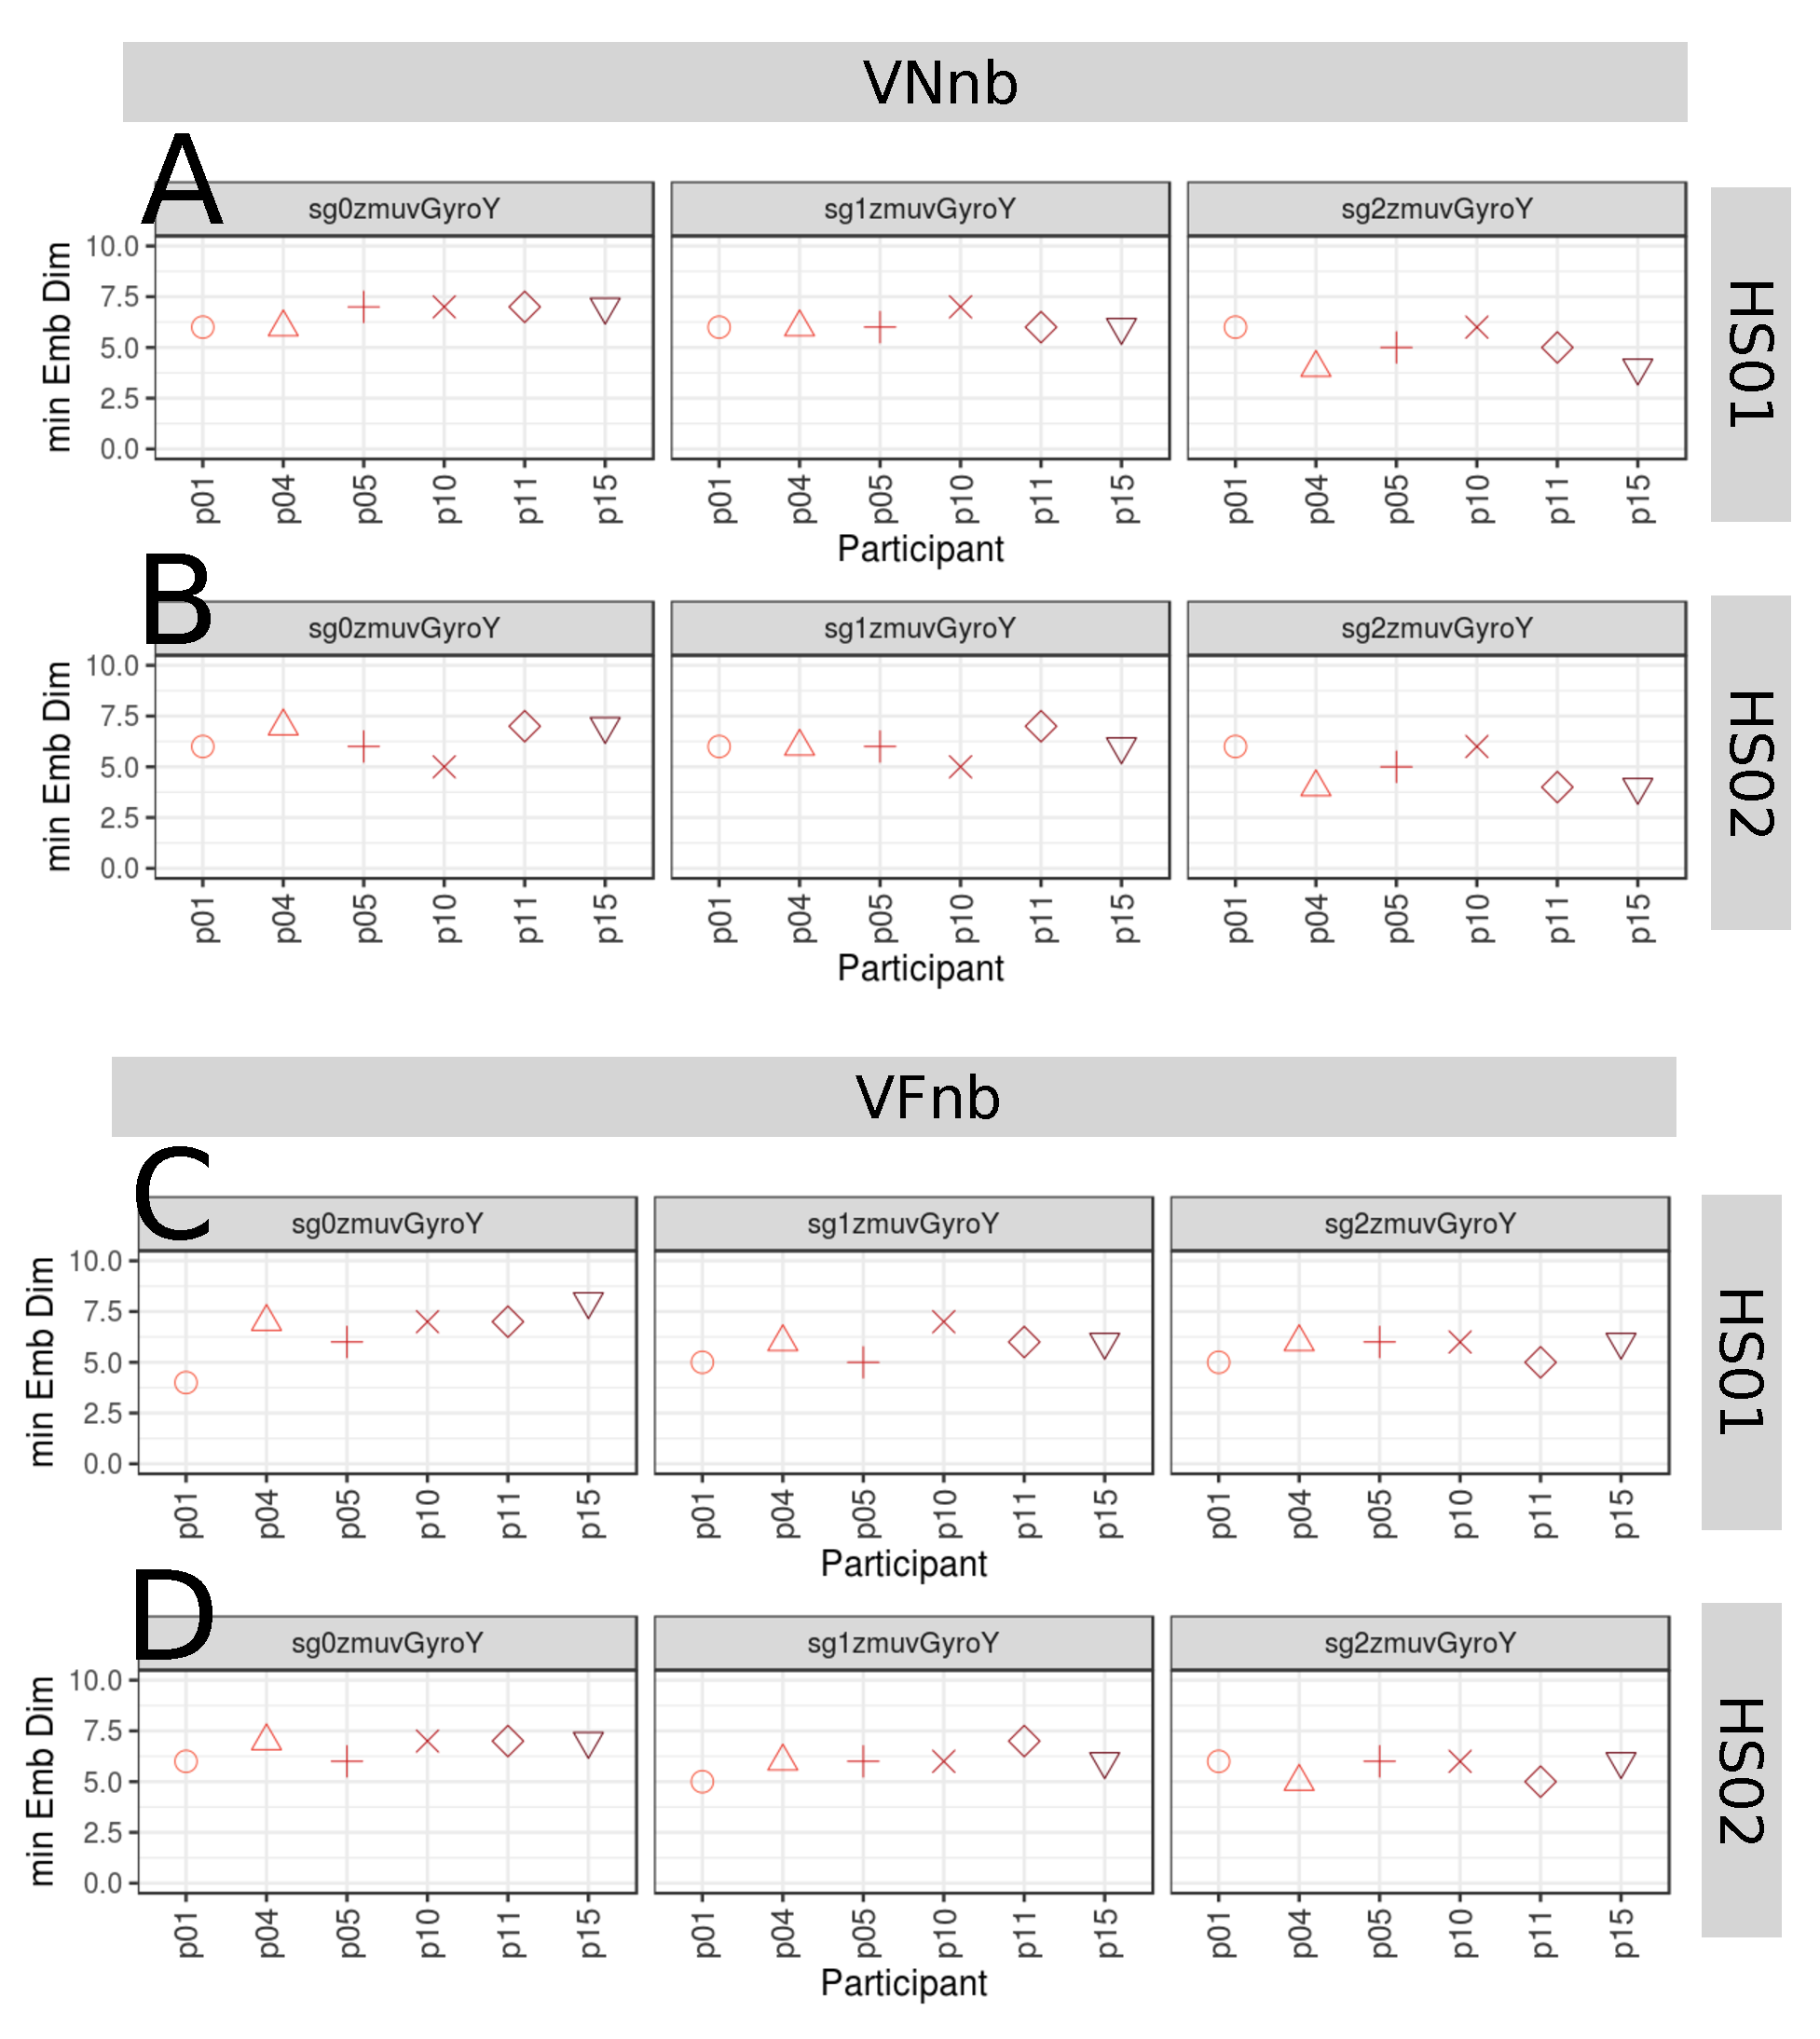
\includegraphics[width=1.0\textwidth]{cao_Vnb_w10}
	\caption
	[Minimum embedding dimensions for vertical arm movements 
	(no beat)]{
	{\bf Minimum embedding dimensions for vertical arm movements 
	(no beat).} 
		(A, B) Vertical Normal with no beat (VNnb), and 
		(C, D) Vertical Faster with no beat (VFnb) movements.
		(A, C) Sensor 01 attached to the participant (HS01), and
		(B, D) sensor 02 attached to the participant (HS02).
		Minimum embedding dimensions are for six participants 
		(p01, p04, p05, p10, p11, p15) with three smoothed signals 
		(sg0zmuvGyroZ, sg1zmuvGyroZ and sg2zmuvGyroZ)
		and window lenght of 10-sec (500 samples).
		R code to reproduce the figure is available 
		from \cite{hwum2018}.
        }
    \label{fig:caoVnb}
\end{figure}
%%---------------------------------(FIGURE)-------------------------------------
%%---------------------------------(FIGURE)-------------------------------------
\begin{figure}
\centering
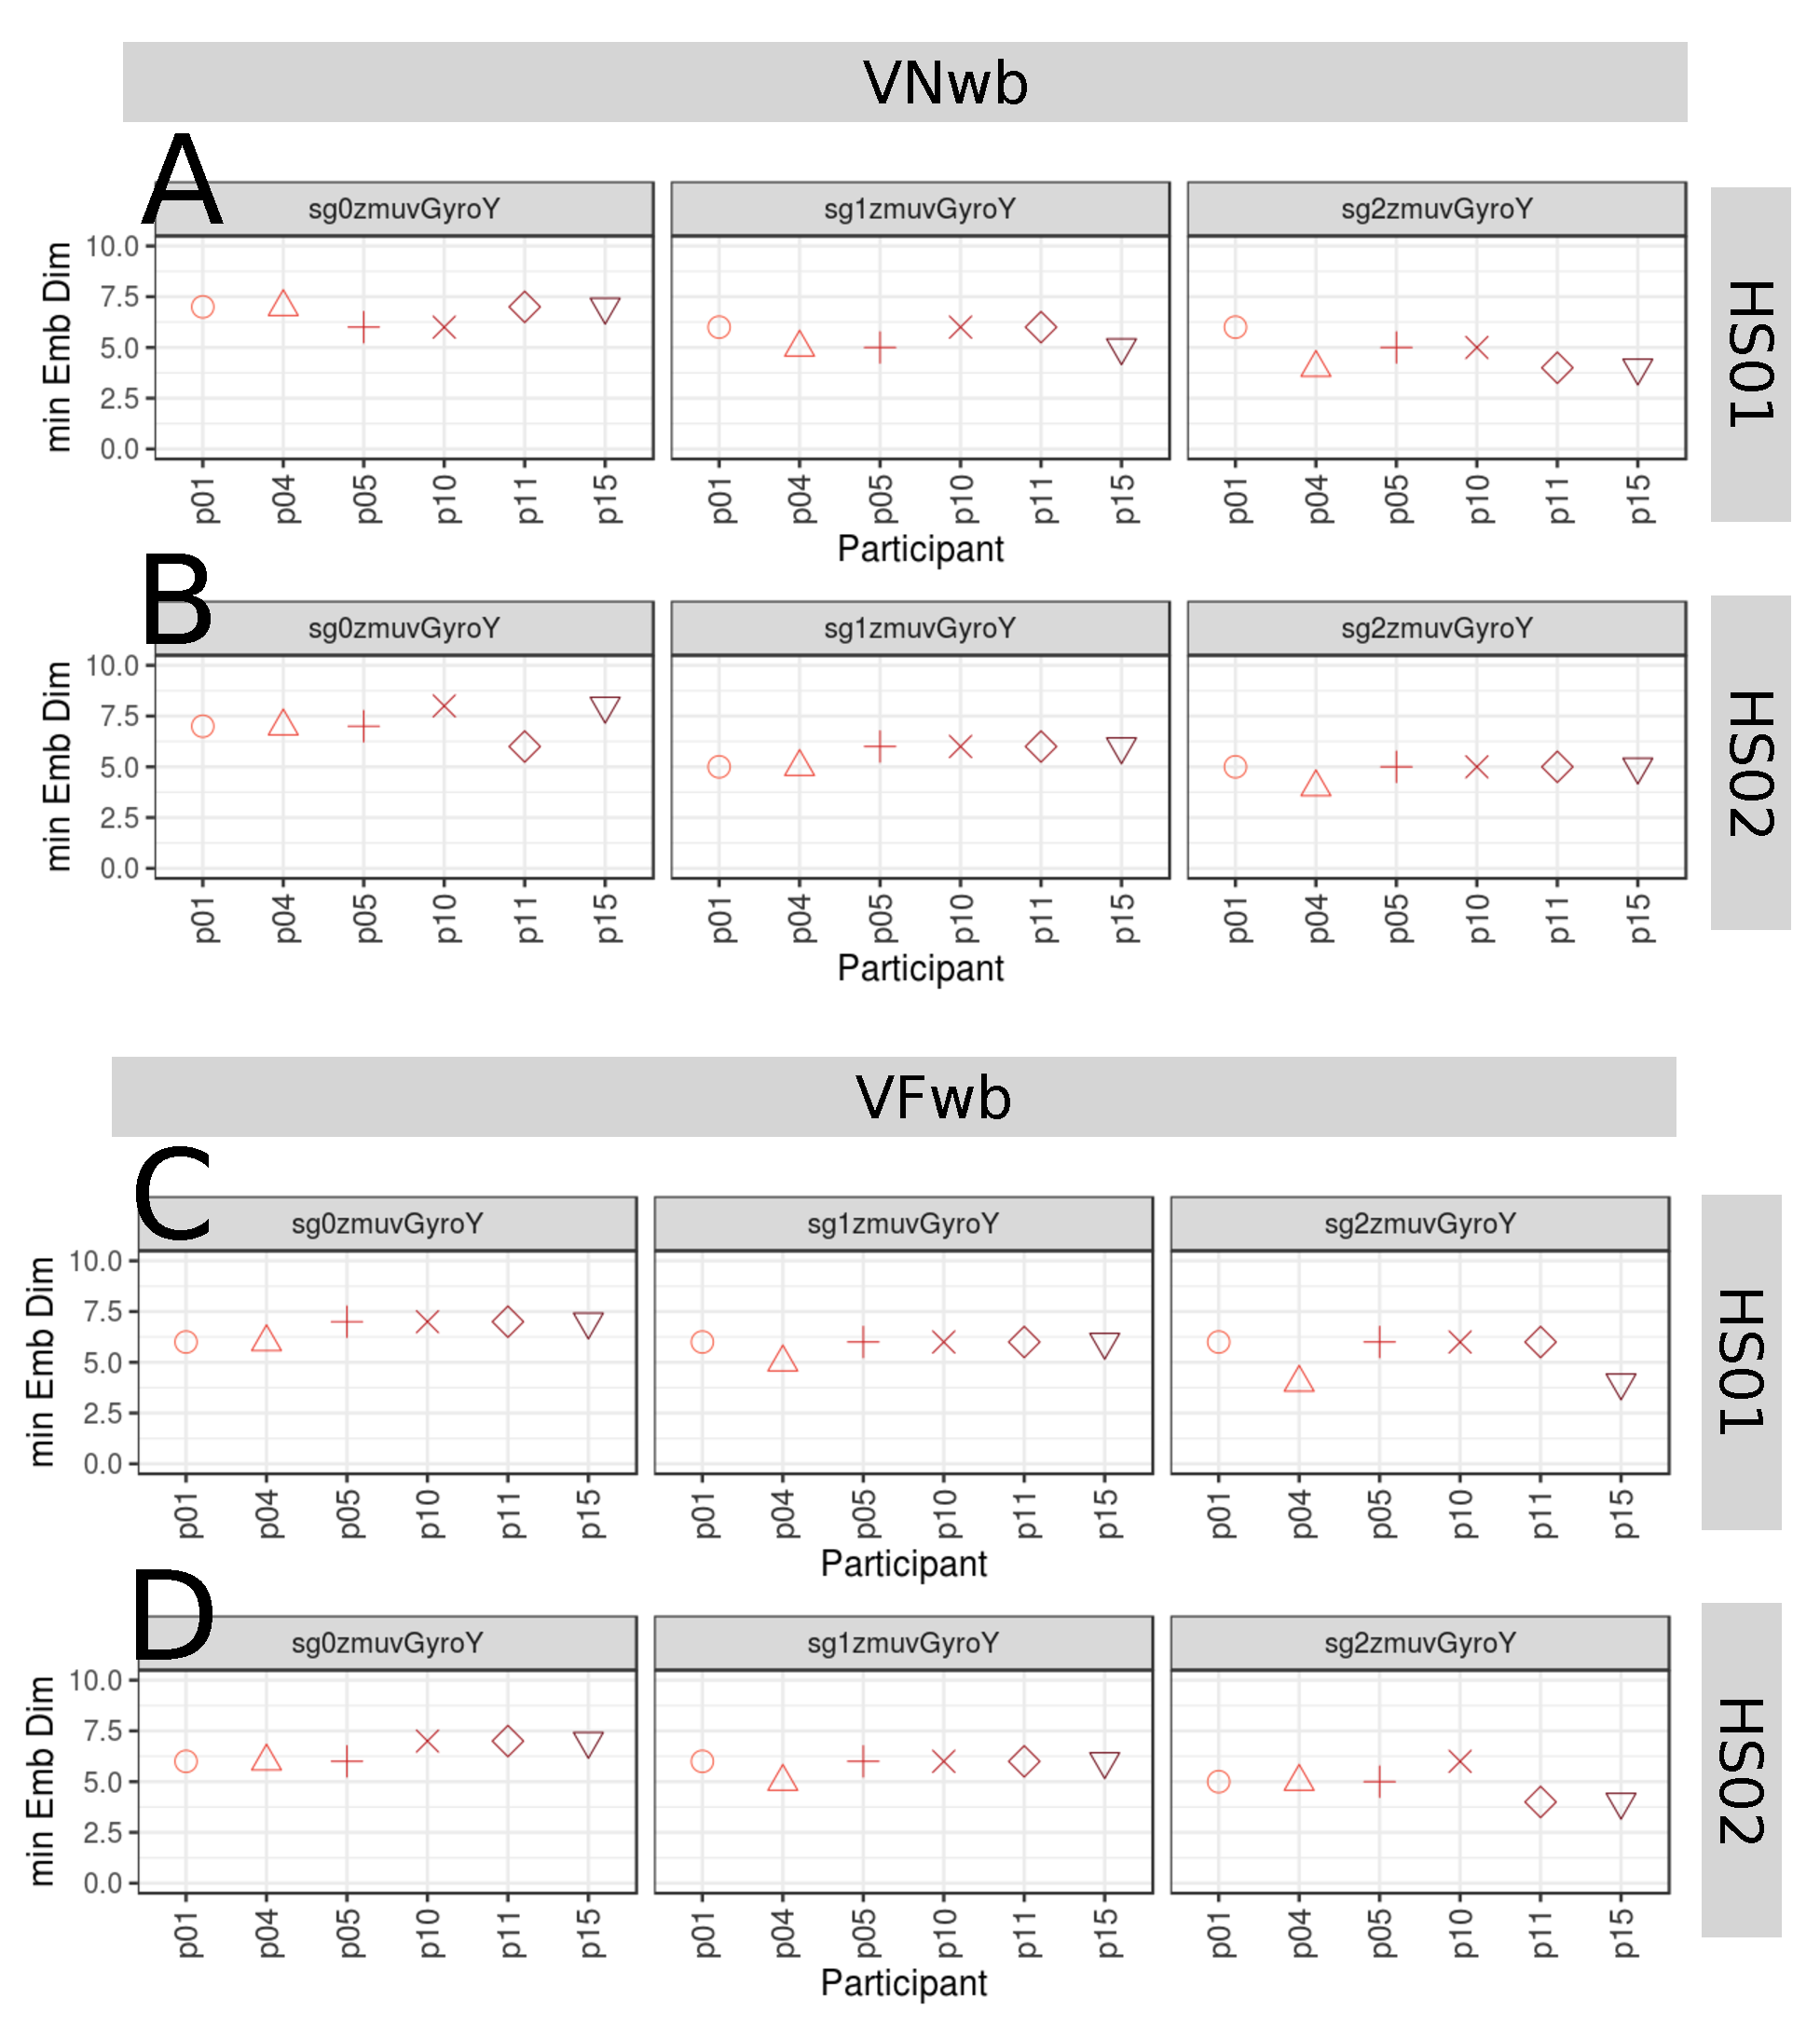
\includegraphics[width=1.0\textwidth]{cao_Vwb_w10}
	\caption
	[Minimum embedding dimensions for vertical arm movements 
	(with beat)]{
	{\bf Minimum embedding dimensions for vertical arm movements 
	(with beat).} 
		(A, B) Vertical Normal with beat (VNwb), and
		(C, D) Vertical Faster with beat (VFwb) movements.
		(A, C) Sensor 01 attached to the participant (HS01), and
		(B, D) sensor 02 attached to the participant (HS02).
		Minimum embedding dimensions are for six participants 
		(p01, p04, p05, p10, p11, p15) with three smoothed signals 
		(sg0zmuvGyroZ, sg1zmuvGyroZ and sg2zmuvGyroZ)
		and window lenght of 10-sec (500 samples).
		R code to reproduce the figure is available 
		from \cite{hwum2018}.
        }
    \label{fig:caoVwb}
\end{figure}
%%---------------------------------(FIGURE)-------------------------------------






\newpage
\subsection{Minimum delay embedding values}

The general behavior for horizontal and vertical arm movements with regards
to the smoothness of the time series is that the first minimum AMI values 
increase as the increase of the smoothness which is due to smoothed AMI 
curves 
(Figs \ref{fig:amiHnb}, \ref{fig:amiHwb}, \ref{fig:amiVnb} and 
\ref{fig:amiVwb}).

Fluctuations of minimum AMI values from sensor HS01 are more evident than 
for sensor HS02 for horizontal normal arm movements with no beat 
(Fig \ref{fig:amiHnb}(A, B)),
whereas fluctuations of minimum AMI values from sensors HS01 and HS02 
for horizontal faster arm movements with no beat appear to be similar 
(Fig \ref{fig:amiHnb}(C, D)).
Similarly, fluctuations of minimum AMI values are more evidently for 
horizontal normal arm movements with beat (Fig \ref{fig:amiHwb}(A, B)) than 
horizontal faster arm movements with beat (Fig \ref{fig:amiHwb}(C, D)).

As smoothness increase, minimum AMI values for vertical normal arm movements 
with no beat appear to fluctuate more (Figs \ref{fig:amiVnb}(A, B))
than vertical faster arm movements with no beat (Figs \ref{fig:amiVnb}(C, D)),
whereas for vertical normal and vertical faster arm movements with beat 
the fluctuation of minimum AMI values is more evidently,
specially when comparing vertical normal arm movements 
(Figs \ref{fig:amiVwb}(A, B)) with vertical faster arm movements 
(Figs \ref{fig:amiVwb}(C, D)).





%%---------------------------------(FIGURE)-------------------------------------
\begin{figure}
\centering
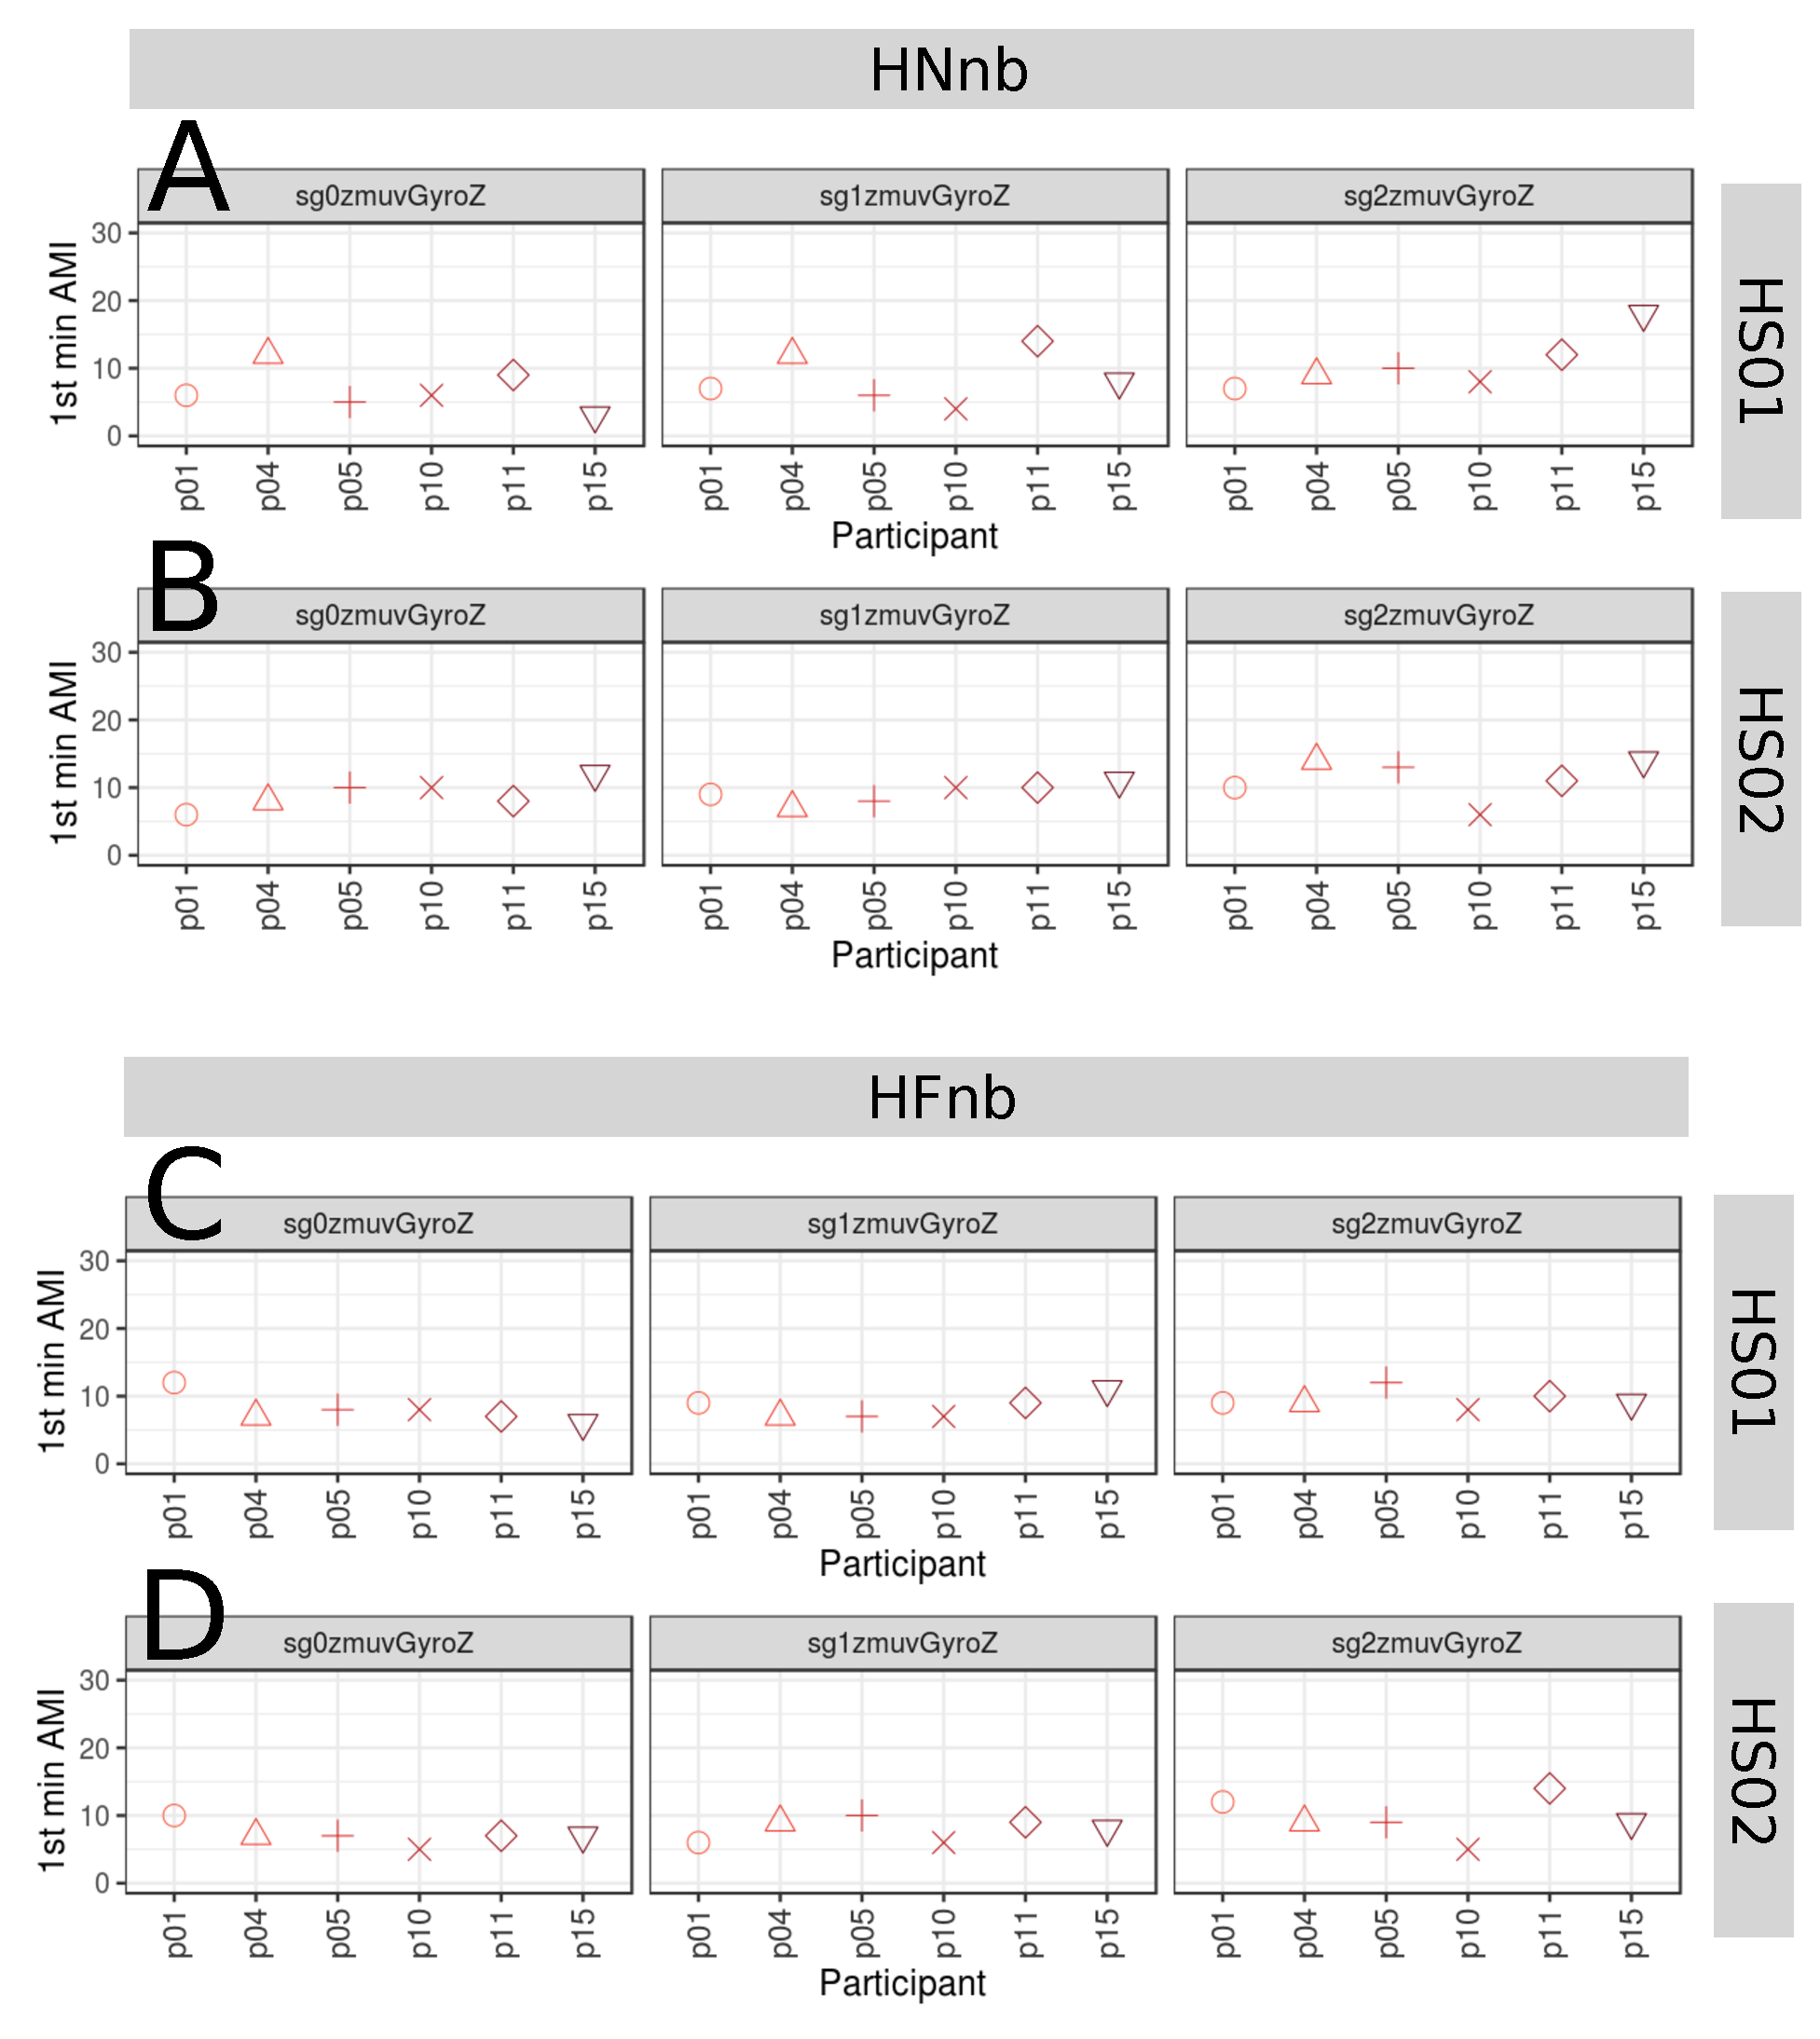
\includegraphics[width=1.0\textwidth]{ami_Hnb_w10}
	\caption
	[First minimum AMI values for horizontal arm movements (no beat)]{
	{\bf First minimum AMI values for horizontal arm movements (no beat).}
		(A, B) Horizontal Normal with no beat (HNnb), and 
		(C, D) Horizontal Faster with no beat (HFnb) movements.
		(A, C) Sensor attached to the participant (HS01), and
		(B, D) sensor attached to the participant (HS02).
		First minimum AMI values are for six participants 
		(p01, p04, p05, p10, p11, p15) with three smoothed 
		signals (sg0zmuvGyroZ, sg1zmuvGyroZ and sg2zmuvGyroZ) and 
		window lenght of 10-sec (500 samples).
		R code to reproduce the figure is available 
		from \cite{hwum2018}.
        }
    \label{fig:amiHnb}
\end{figure}
%%---------------------------------(FIGURE)------------------------------------
%%---------------------------------(FIGURE)-------------------------------------
\begin{figure}
\centering
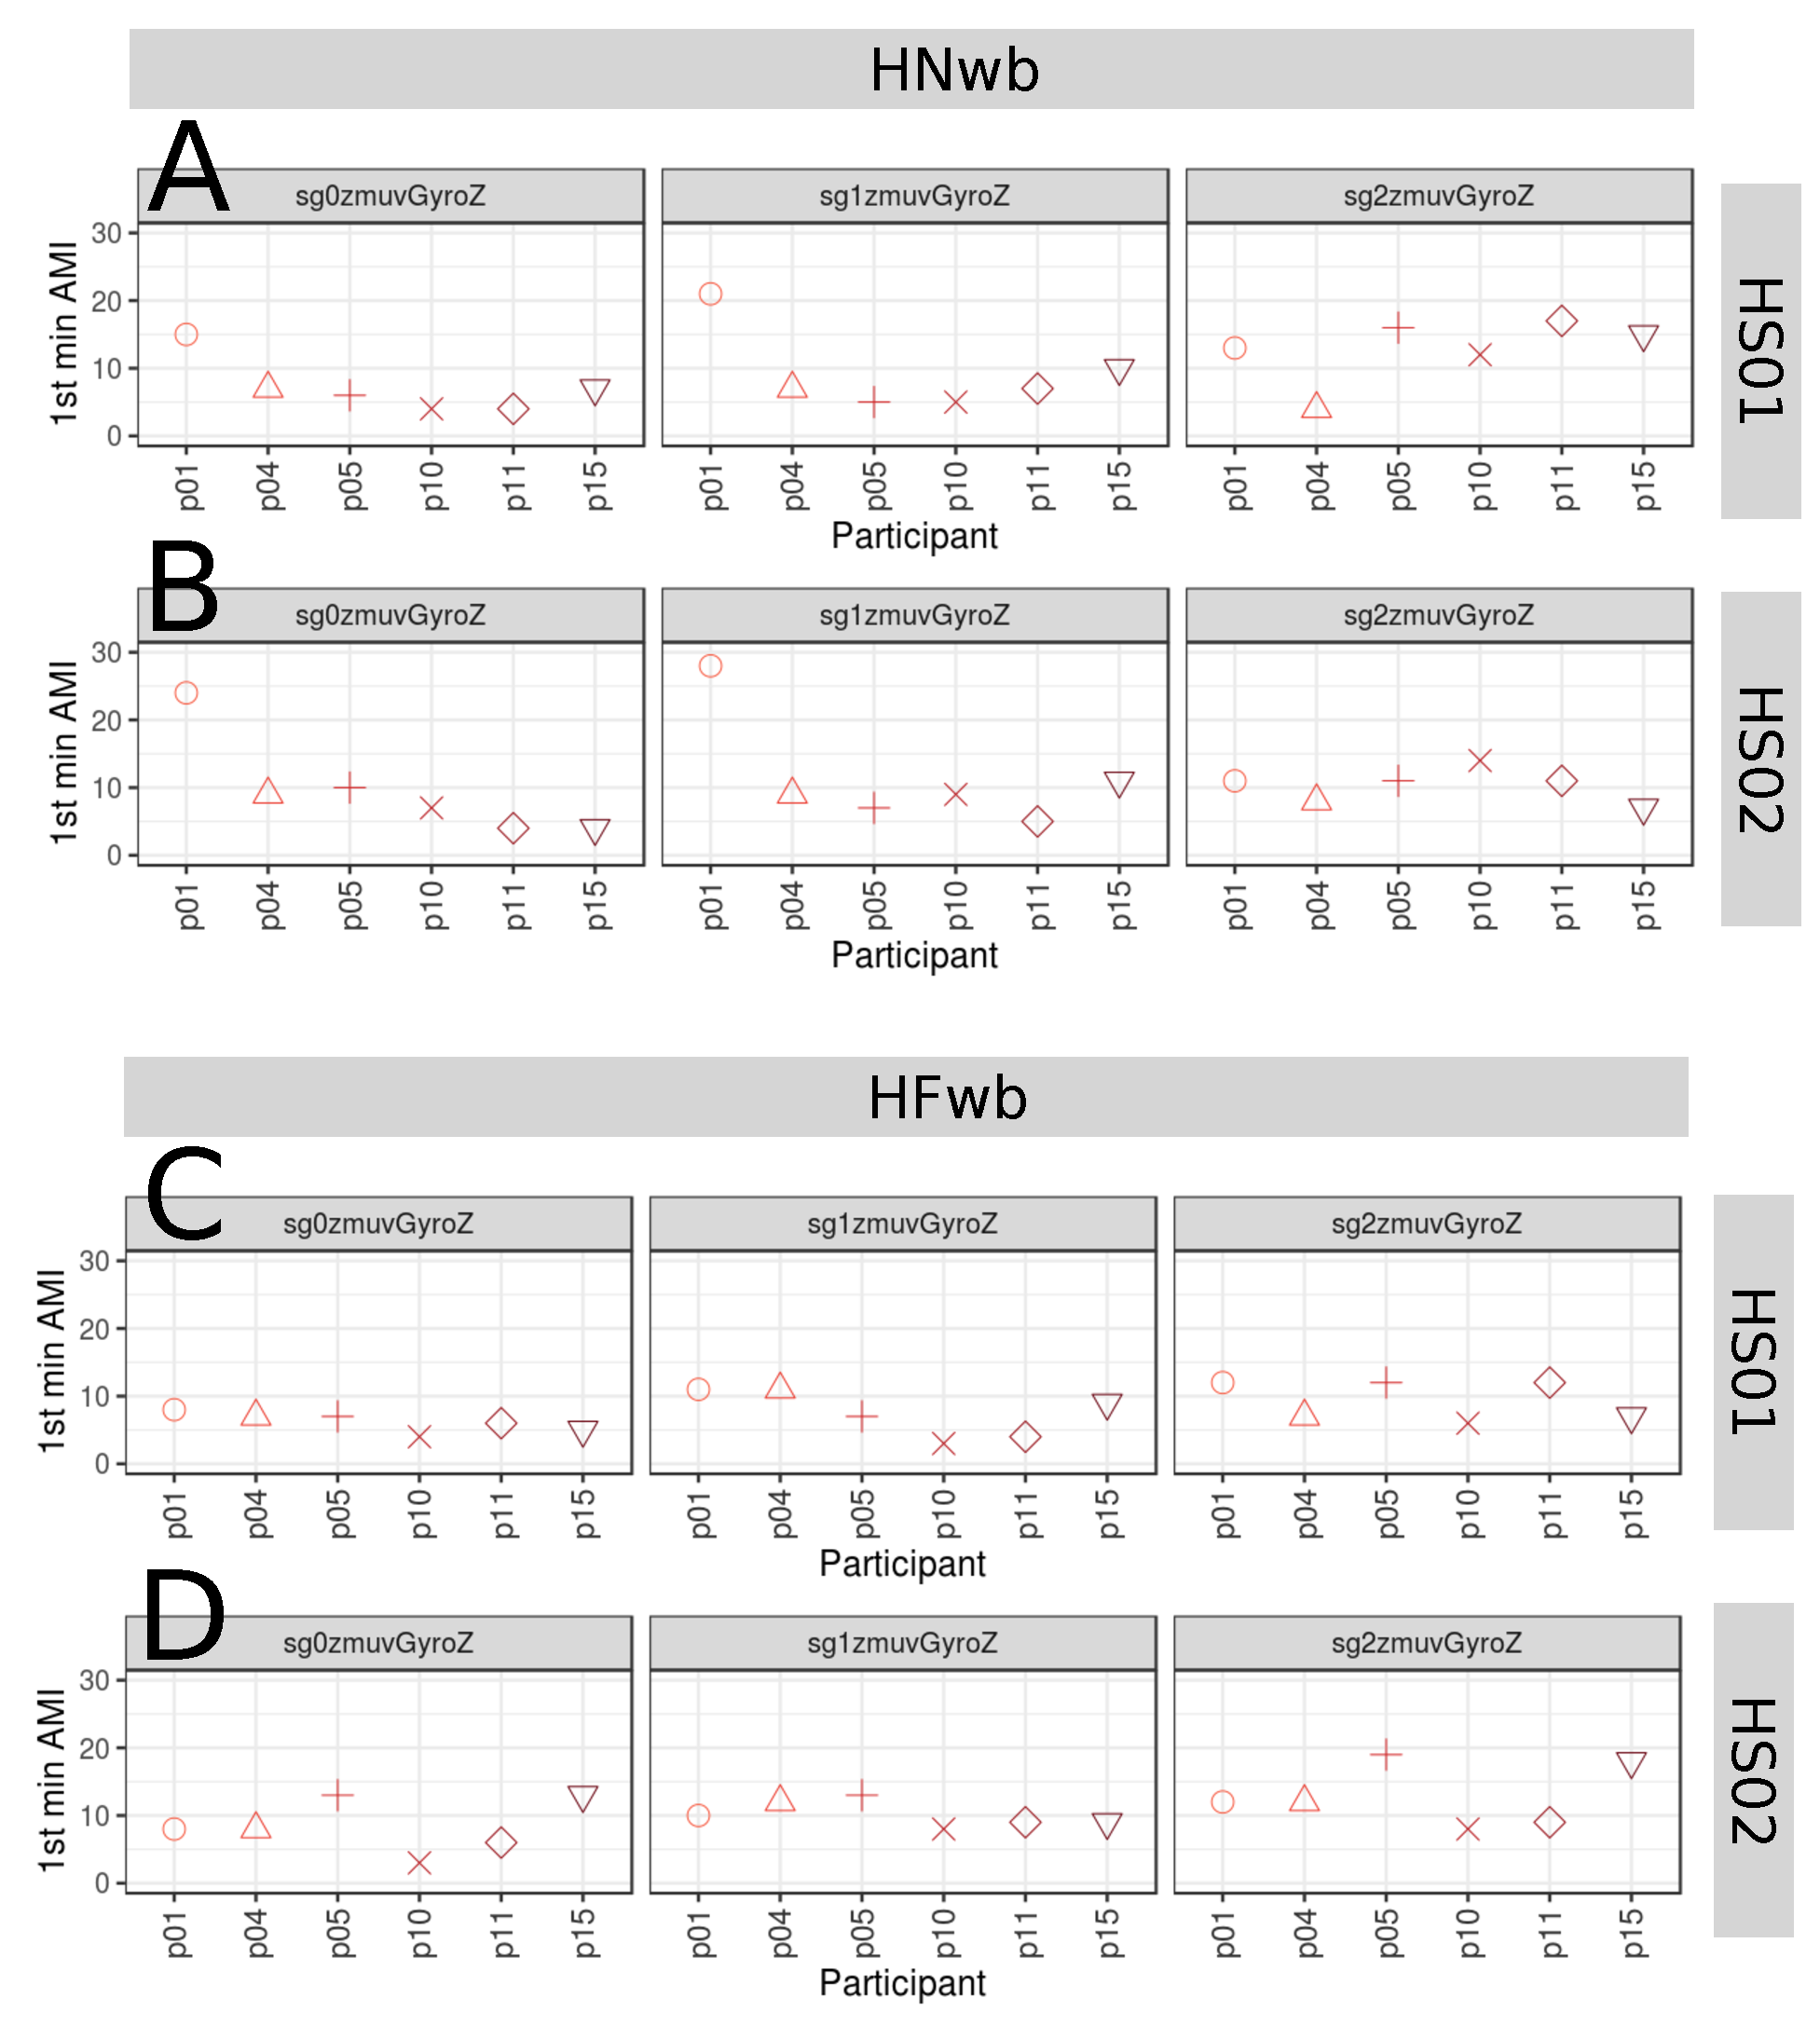
\includegraphics[width=1.0\textwidth]{ami_Hwb_w10}
	\caption
	[First minimum AMI values for horizontal arm movements (with beat)]{
	{\bf First minimum AMI values for horizontal arm movements (with beat).}
		(A, B) Horizontal Normal with beat (HNwb), and 
		(C, D) Horizontal Faster with beat (HFwb) movements.
		(A, C) Sensor attached to the participant (HS01), and
		(B, D) sensor attached to the participant (HS02).
		First minimum AMI values are for six participants 
		(p01, p04, p05, p10, p11, p15) with three smoothed 
		signals (sg0zmuvGyroZ, sg1zmuvGyroZ and sg2zmuvGyroZ) and 
		window lenght of 10-sec (500 samples).
		R code to reproduce the figure is available 
		from \cite{hwum2018}.
        }
    \label{fig:amiHwb}
\end{figure}
%%---------------------------------(FIGURE)------------------------------------

%%---------------------------------(FIGURE)------------------------------------
\begin{figure}
\centering
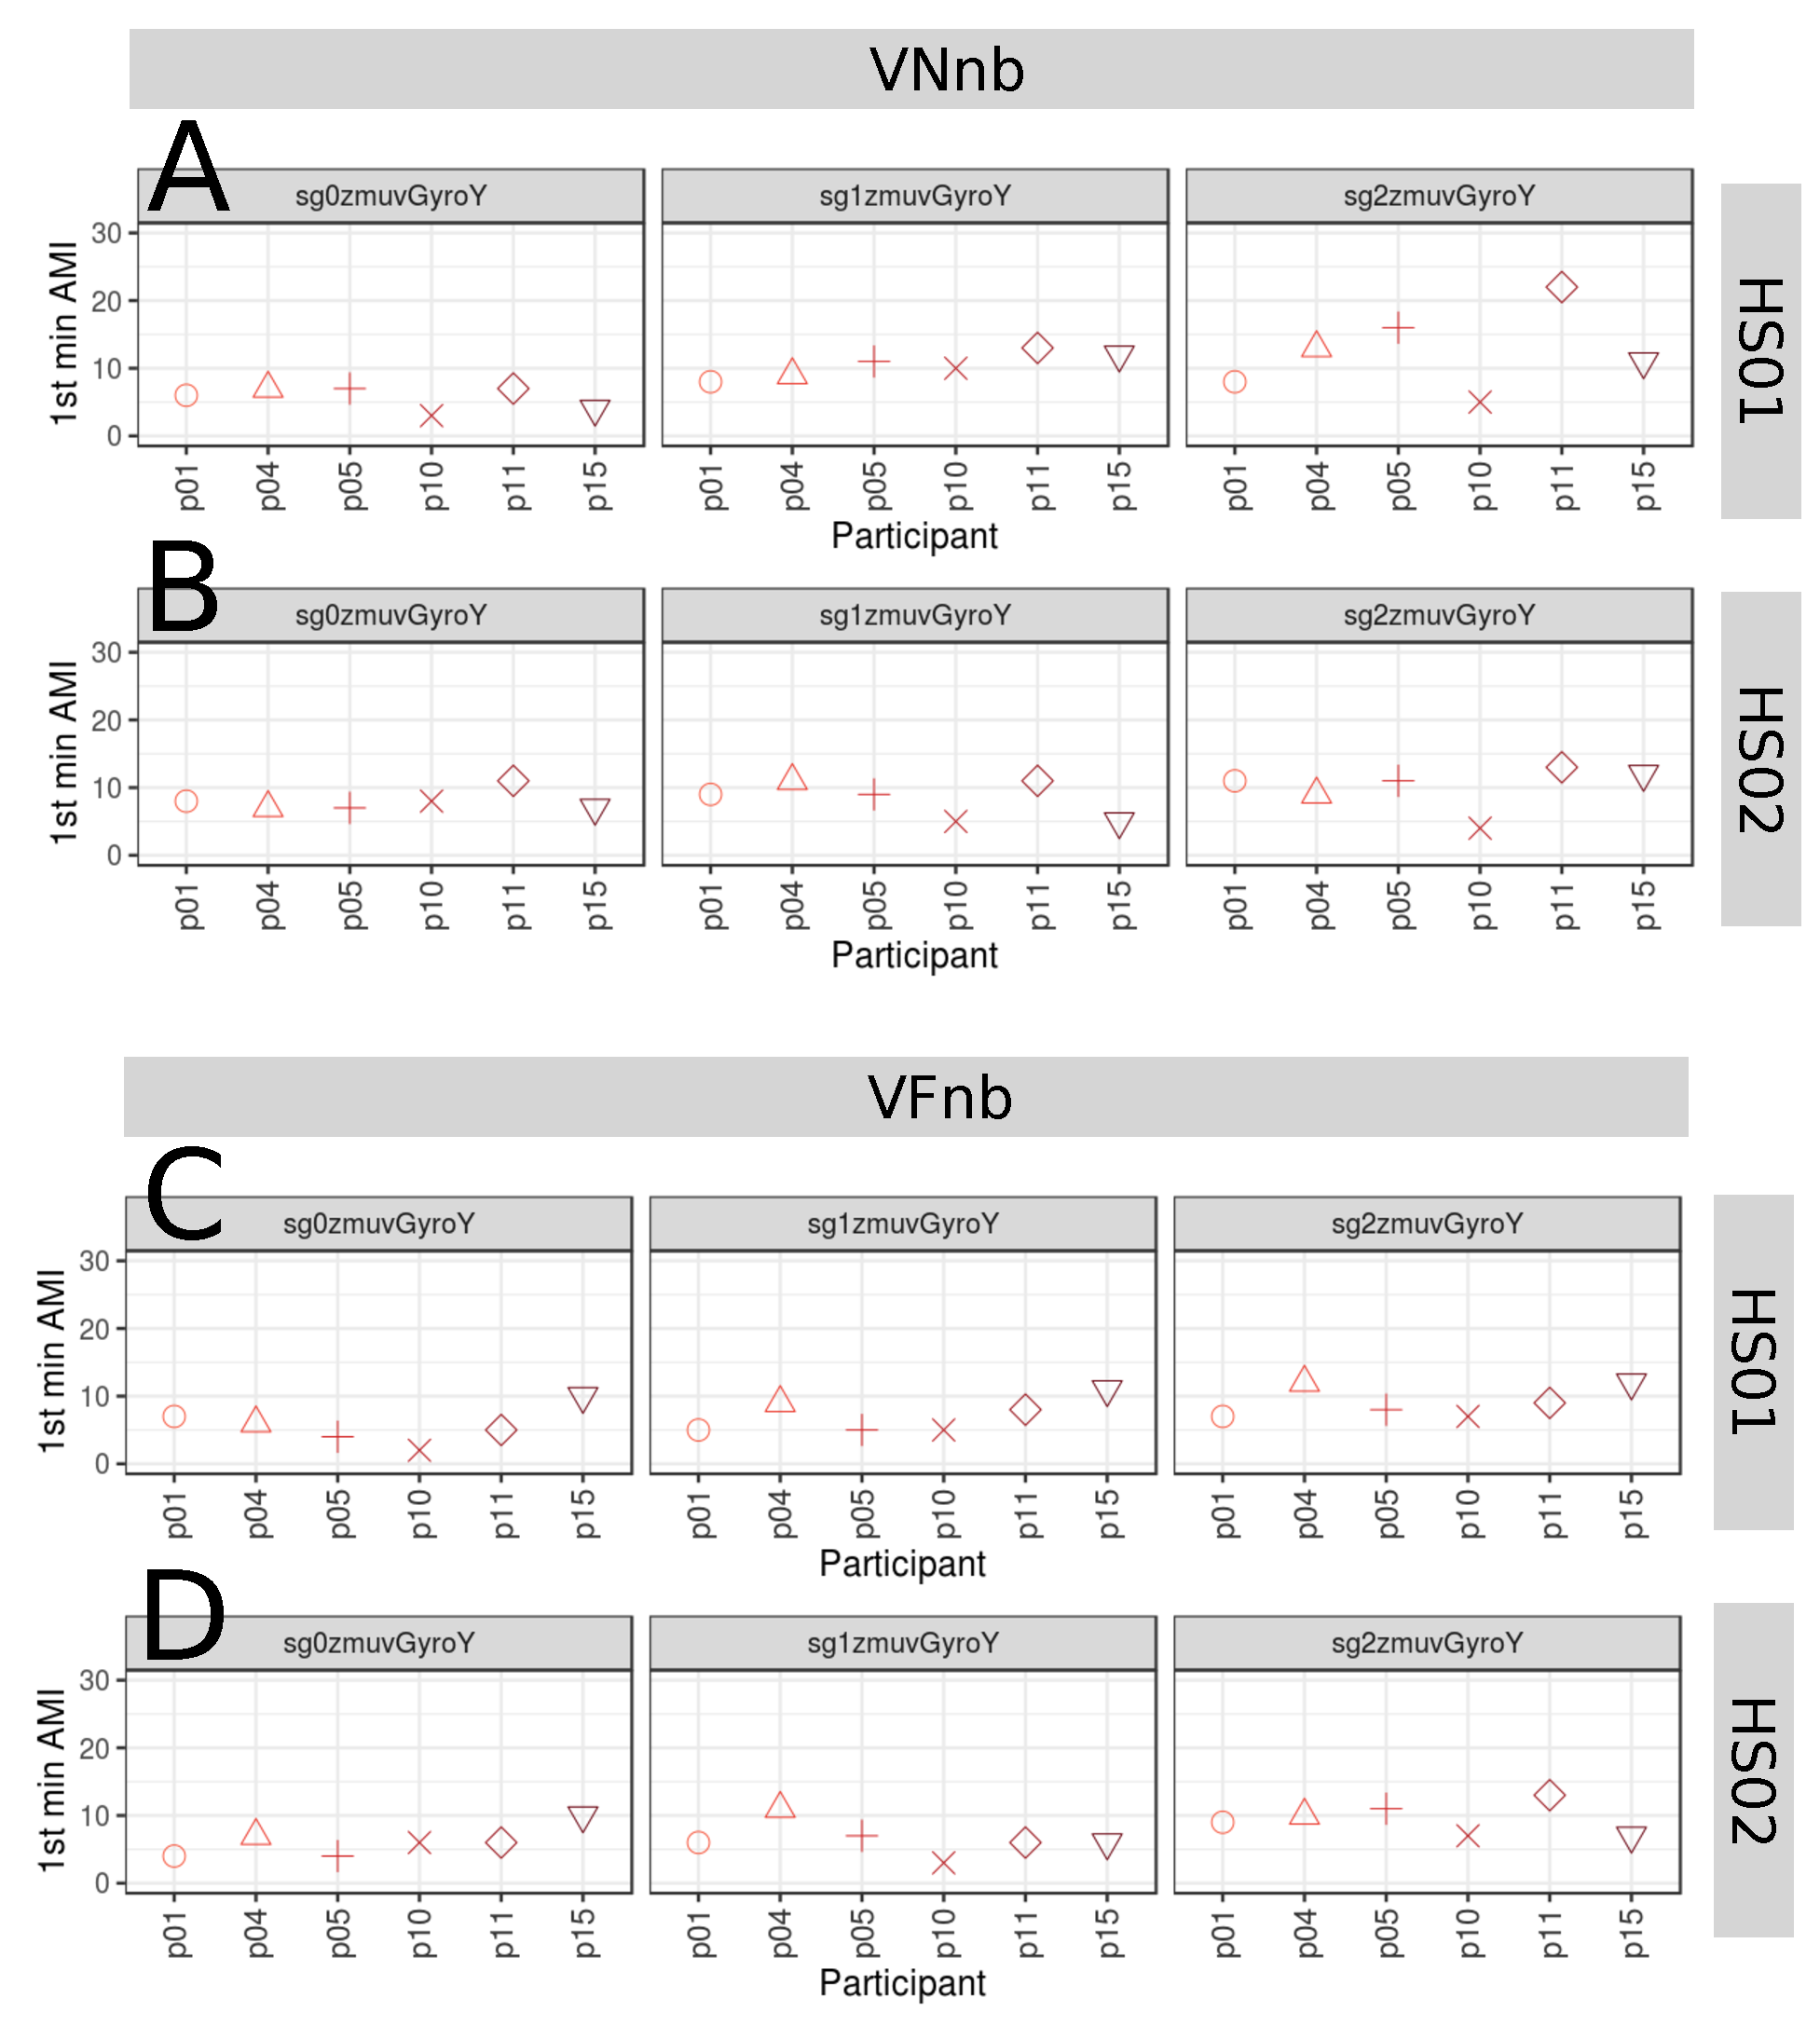
\includegraphics[width=1.0\textwidth]{ami_Vnb_w10}
	\caption
	[First minimum AMI values for vertical arm movements (no beat)]{
	{\bf First minimum AMI values for vertical arm movements (no beat).}
		(A, B) Vertical Normal with no beat (VNnb), and 
		(C, D) Vertical Faster with no beat (VFnb) movements.
		(A, C) Sensor attached to the participant (HS01), and
		(B, D) sensor attached to the participant (HS02).
		First minimum AMI values are for six participants 
		(p01, p04, p05, p10, p11, p15) with three smoothed 
		signals (sg0zmuvGyroZ, sg1zmuvGyroZ and sg2zmuvGyroZ) and 
		window lenght of 10-sec (500 samples).
		R code to reproduce the figure is available 
		from \cite{hwum2018}.
        }
    \label{fig:amiVnb}
\end{figure}
%%---------------------------------(FIGURE)------------------------------------

%%---------------------------------(FIGURE)------------------------------------
\begin{figure}
\centering
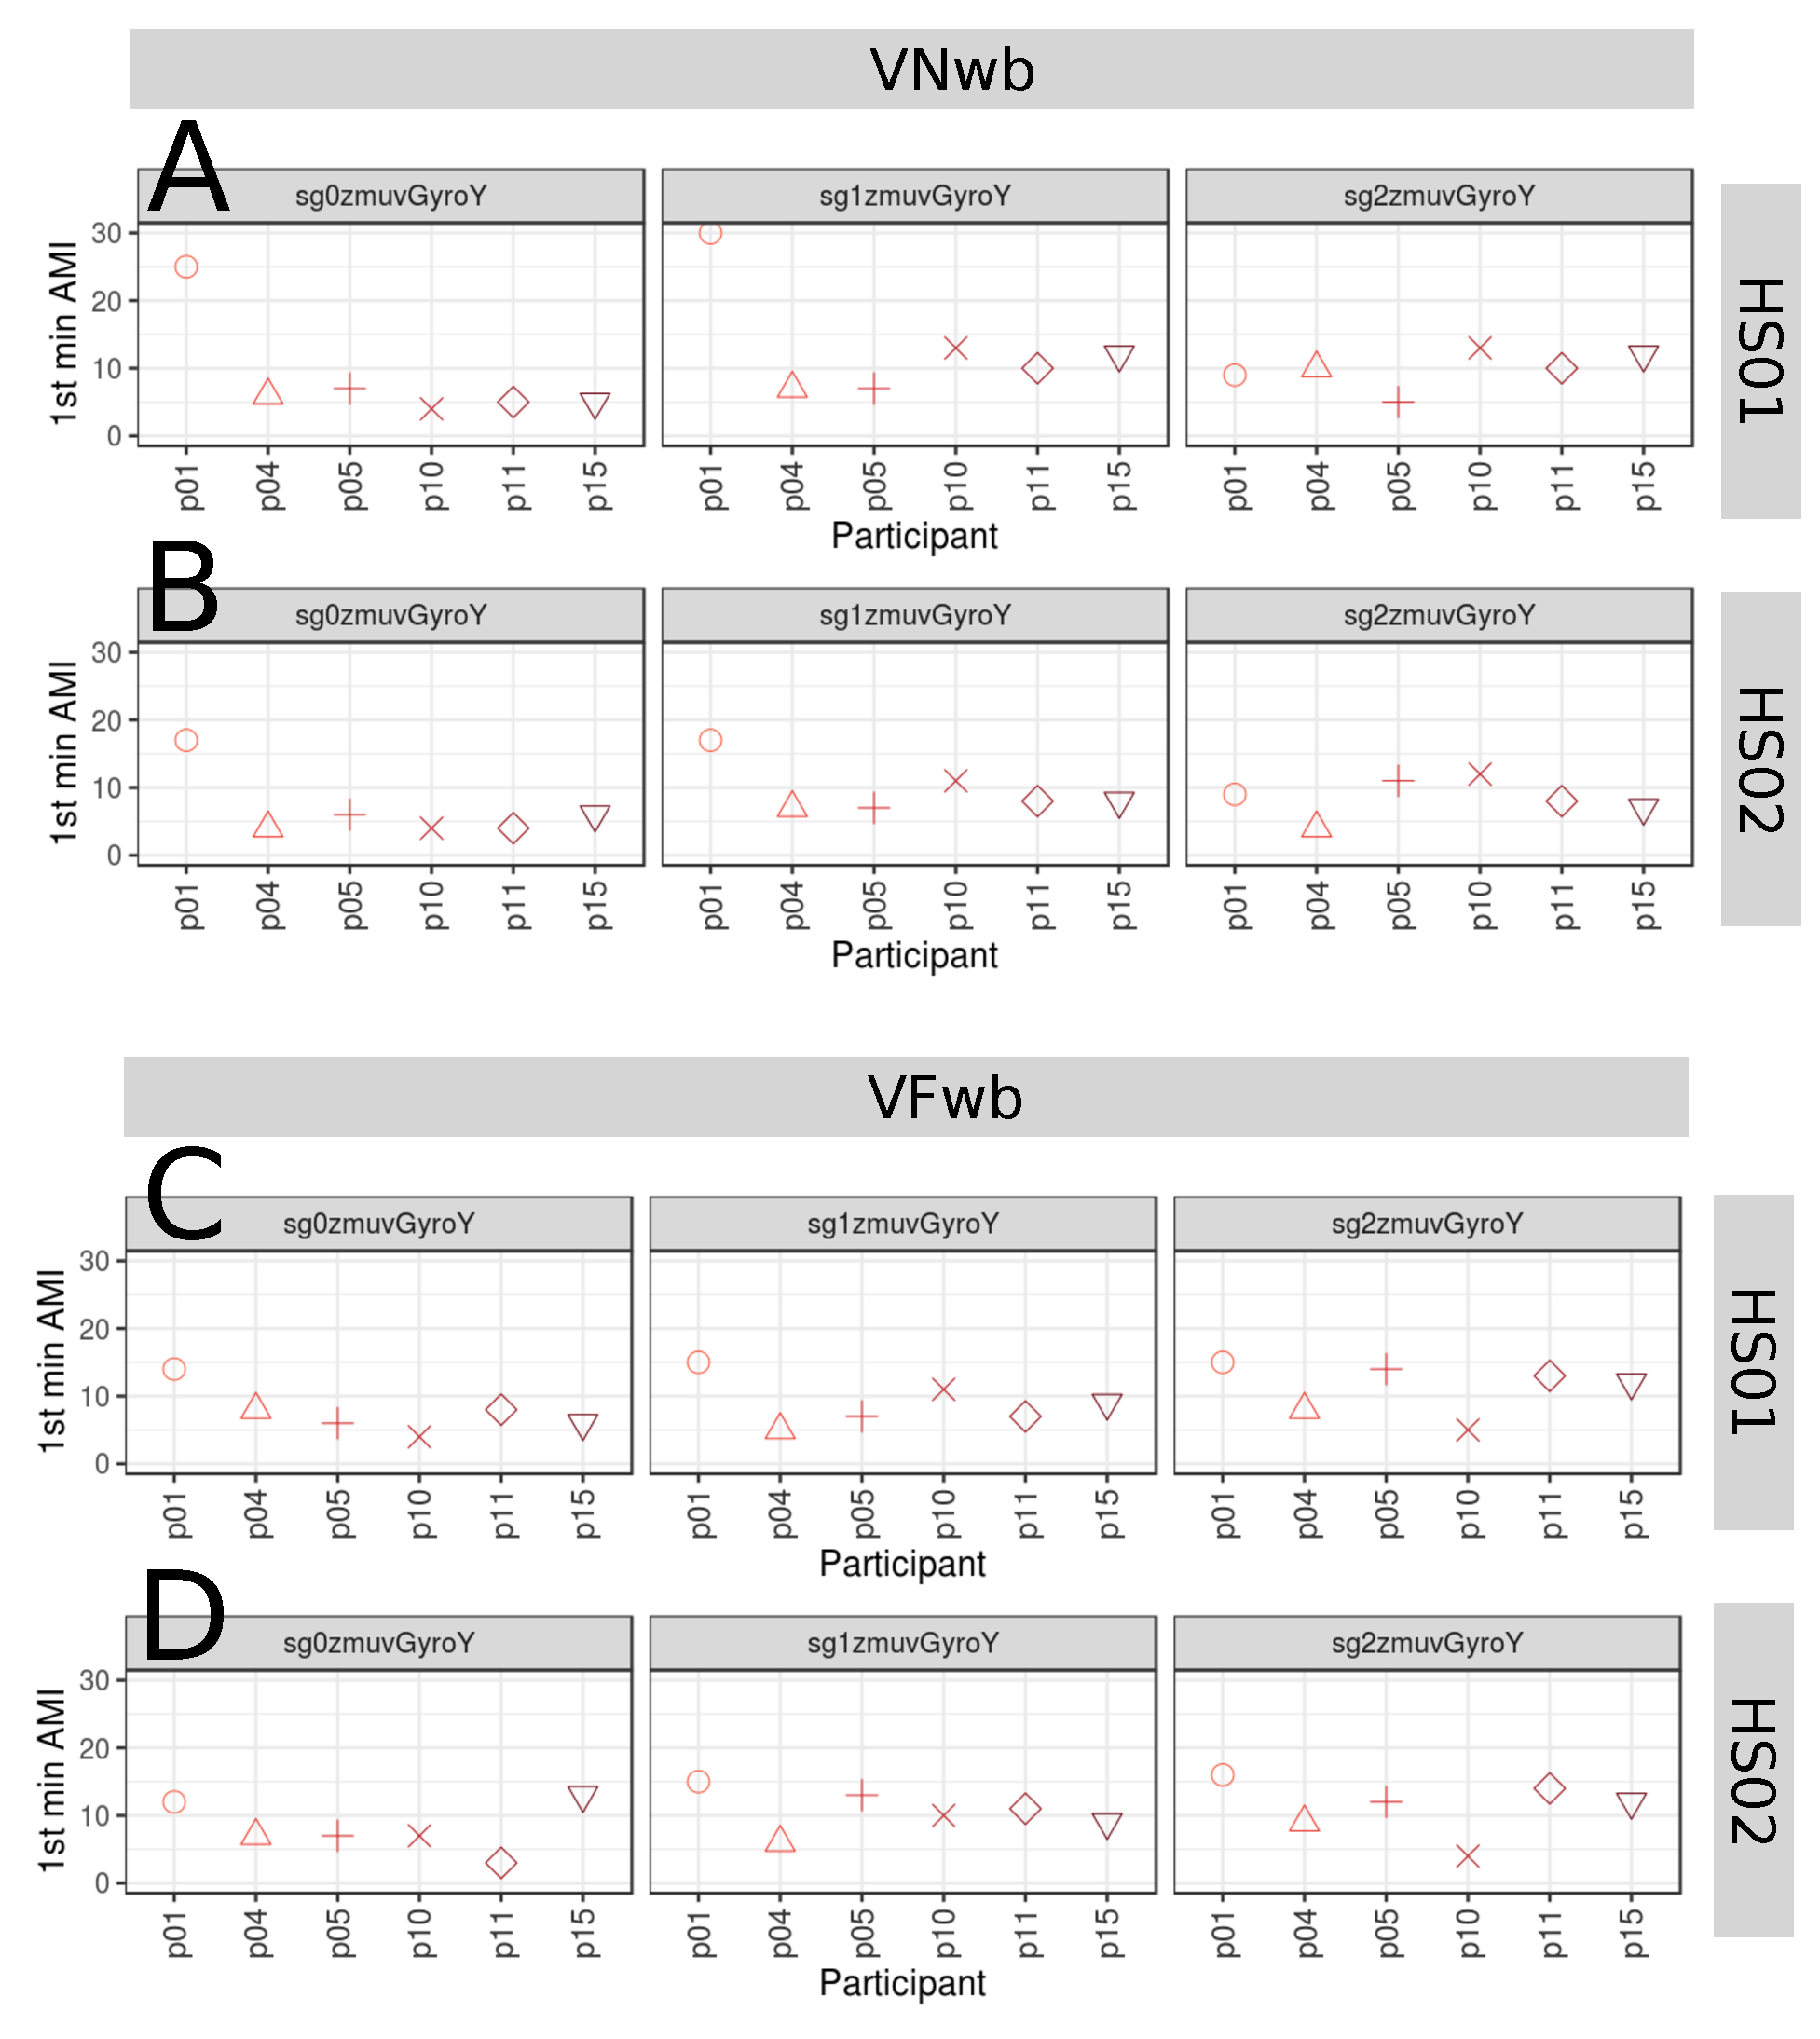
\includegraphics[width=1.0\textwidth]{ami_Vwb_w10}
	\caption
	[First minimum AMI values for vertical arm movements (with beat)]{
	{\bf First minimum AMI values for vertical arm movements (with beat).}
		(A, B) Vertical Normal with beat (VNwb), and 
		(C, D) Vertical Faster with beat (VFwb) movements.
		(A, C) Sensor attached to the participant (HS01), and
		(B, D) sensor attached to the participant (HS02).
		First minimum AMI values are for six participants 
		(p01, p04, p05, p10, p11, p15) with three smoothed 
		signals (sg0zmuvGyroZ, sg1zmuvGyroZ and sg2zmuvGyroZ) and 
		window lenght of 10-sec (500 samples).
		R code to reproduce the figure is available 
		from \cite{hwum2018}.
        }
    \label{fig:amiVwb}
\end{figure}
%%---------------------------------(FIGURE)------------------------------------












\newpage
\section{RSSs} \label{appendix:d:rsss}

The following Figs.  
\ref{fig:rss_HFnb_p04},
\ref{fig:rss_HFwb_p04},
\ref{fig:rss_HNnb_p04},
\ref{fig:rss_HNwb_p04},
\ref{fig:rss_VFnb_p04},
\ref{fig:rss_VFwb_p04},
\ref{fig:rss_VNnb_p04},
\ref{fig:rss_VNwb_p04} 
illustrate reconstructed state spaces 
of participant $p04$ with a window length size of 500 samples.
We refer the reader to download the data and code at \cite{hwum2018}
for the remained window size lengths and other participants.



%%%%%%%%%HORIZONTAL

%%---------------------------------(FIGURE)-------------------------------------
\begin{figure}
\centering
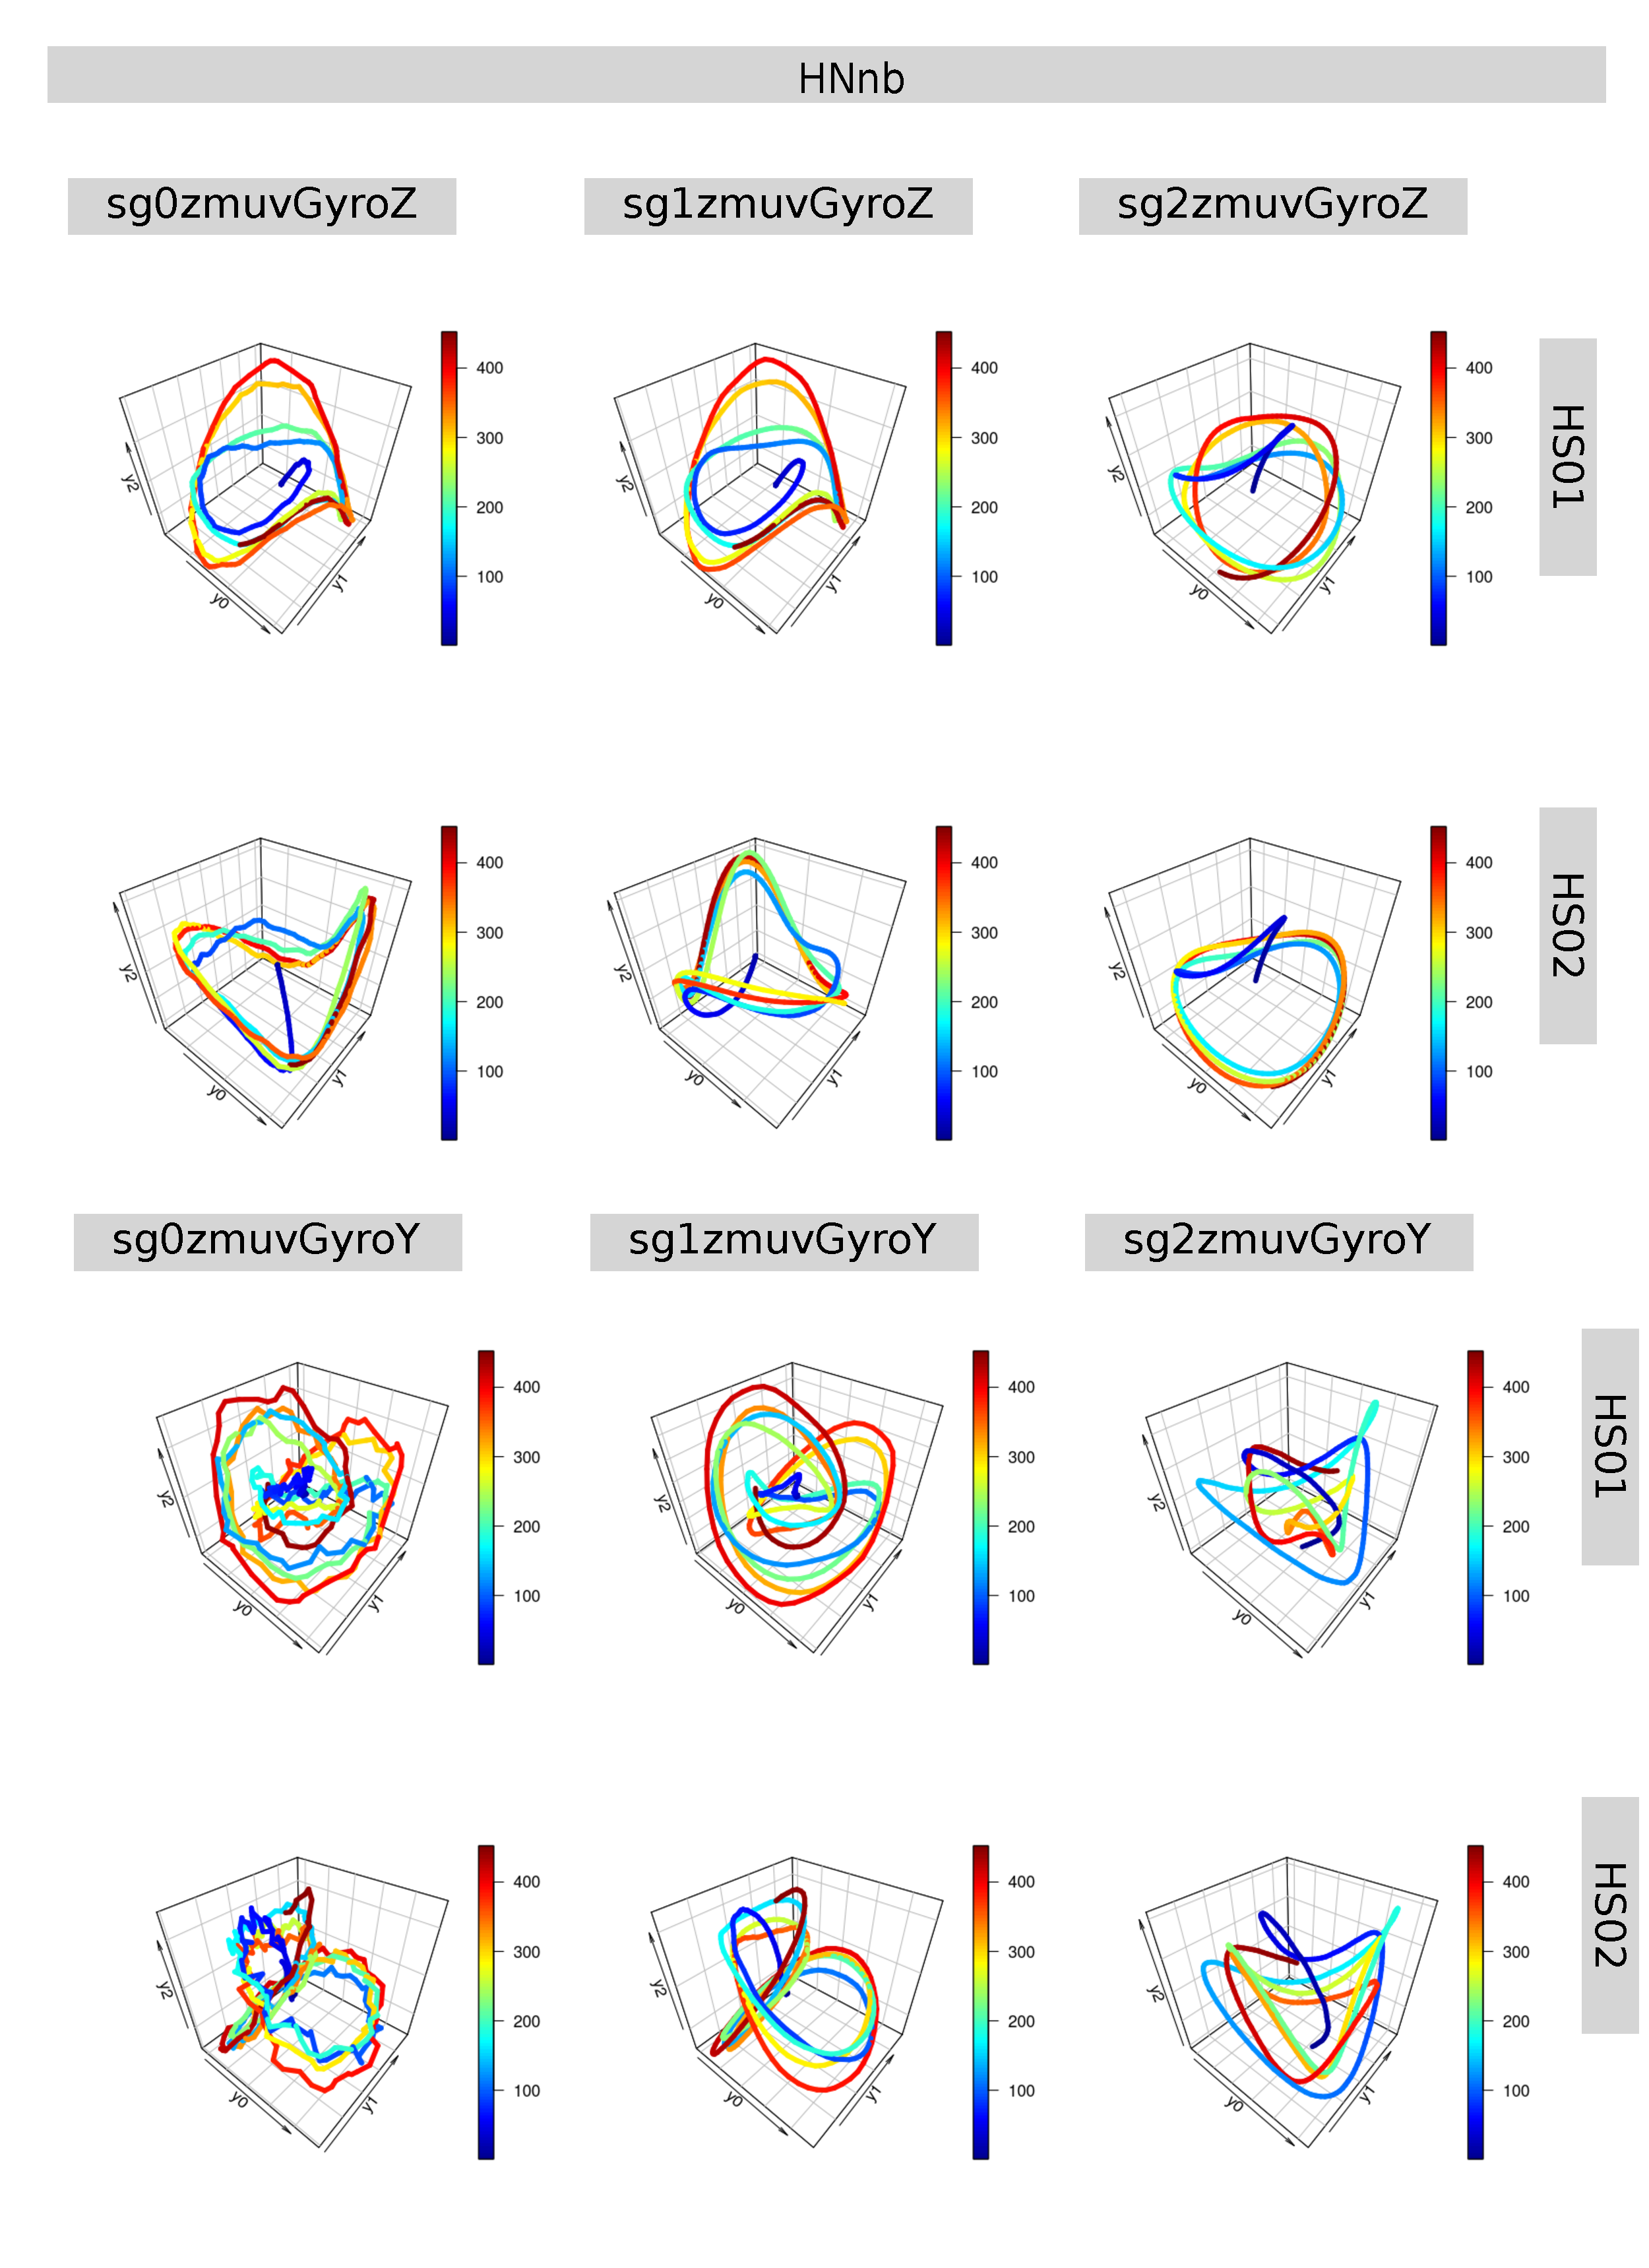
\includegraphics[height=0.8\textheight]{rss_HNnb_p04}
\caption
	[RSSs for horizontal normal arm movements (no beat)]{
	{\bf RSSs for horizontal normal arm movements (no beat).}
	Reconstructed state spaces of participant $p04$
	with time series for raw-normalised (sg0), 
	normalised-smoothed 1 (sg1) and 
	normalised-smoothed 2 (sg2), 
	with sensors attached to the participant (HS01, HS02).
	Reconstructed state spaces were computed with 
	embedding parameters $m=9$, $\tau=6$.
	R code to reproduce the figure is available from \cite{hwum2018}.
        }
     \label{fig:rss_HNnb_p04}
\end{figure}
%%---------------------------------(FIGURE)------------------------------------



%%---------------------------------(FIGURE)-------------------------------------
\begin{figure}
\centering
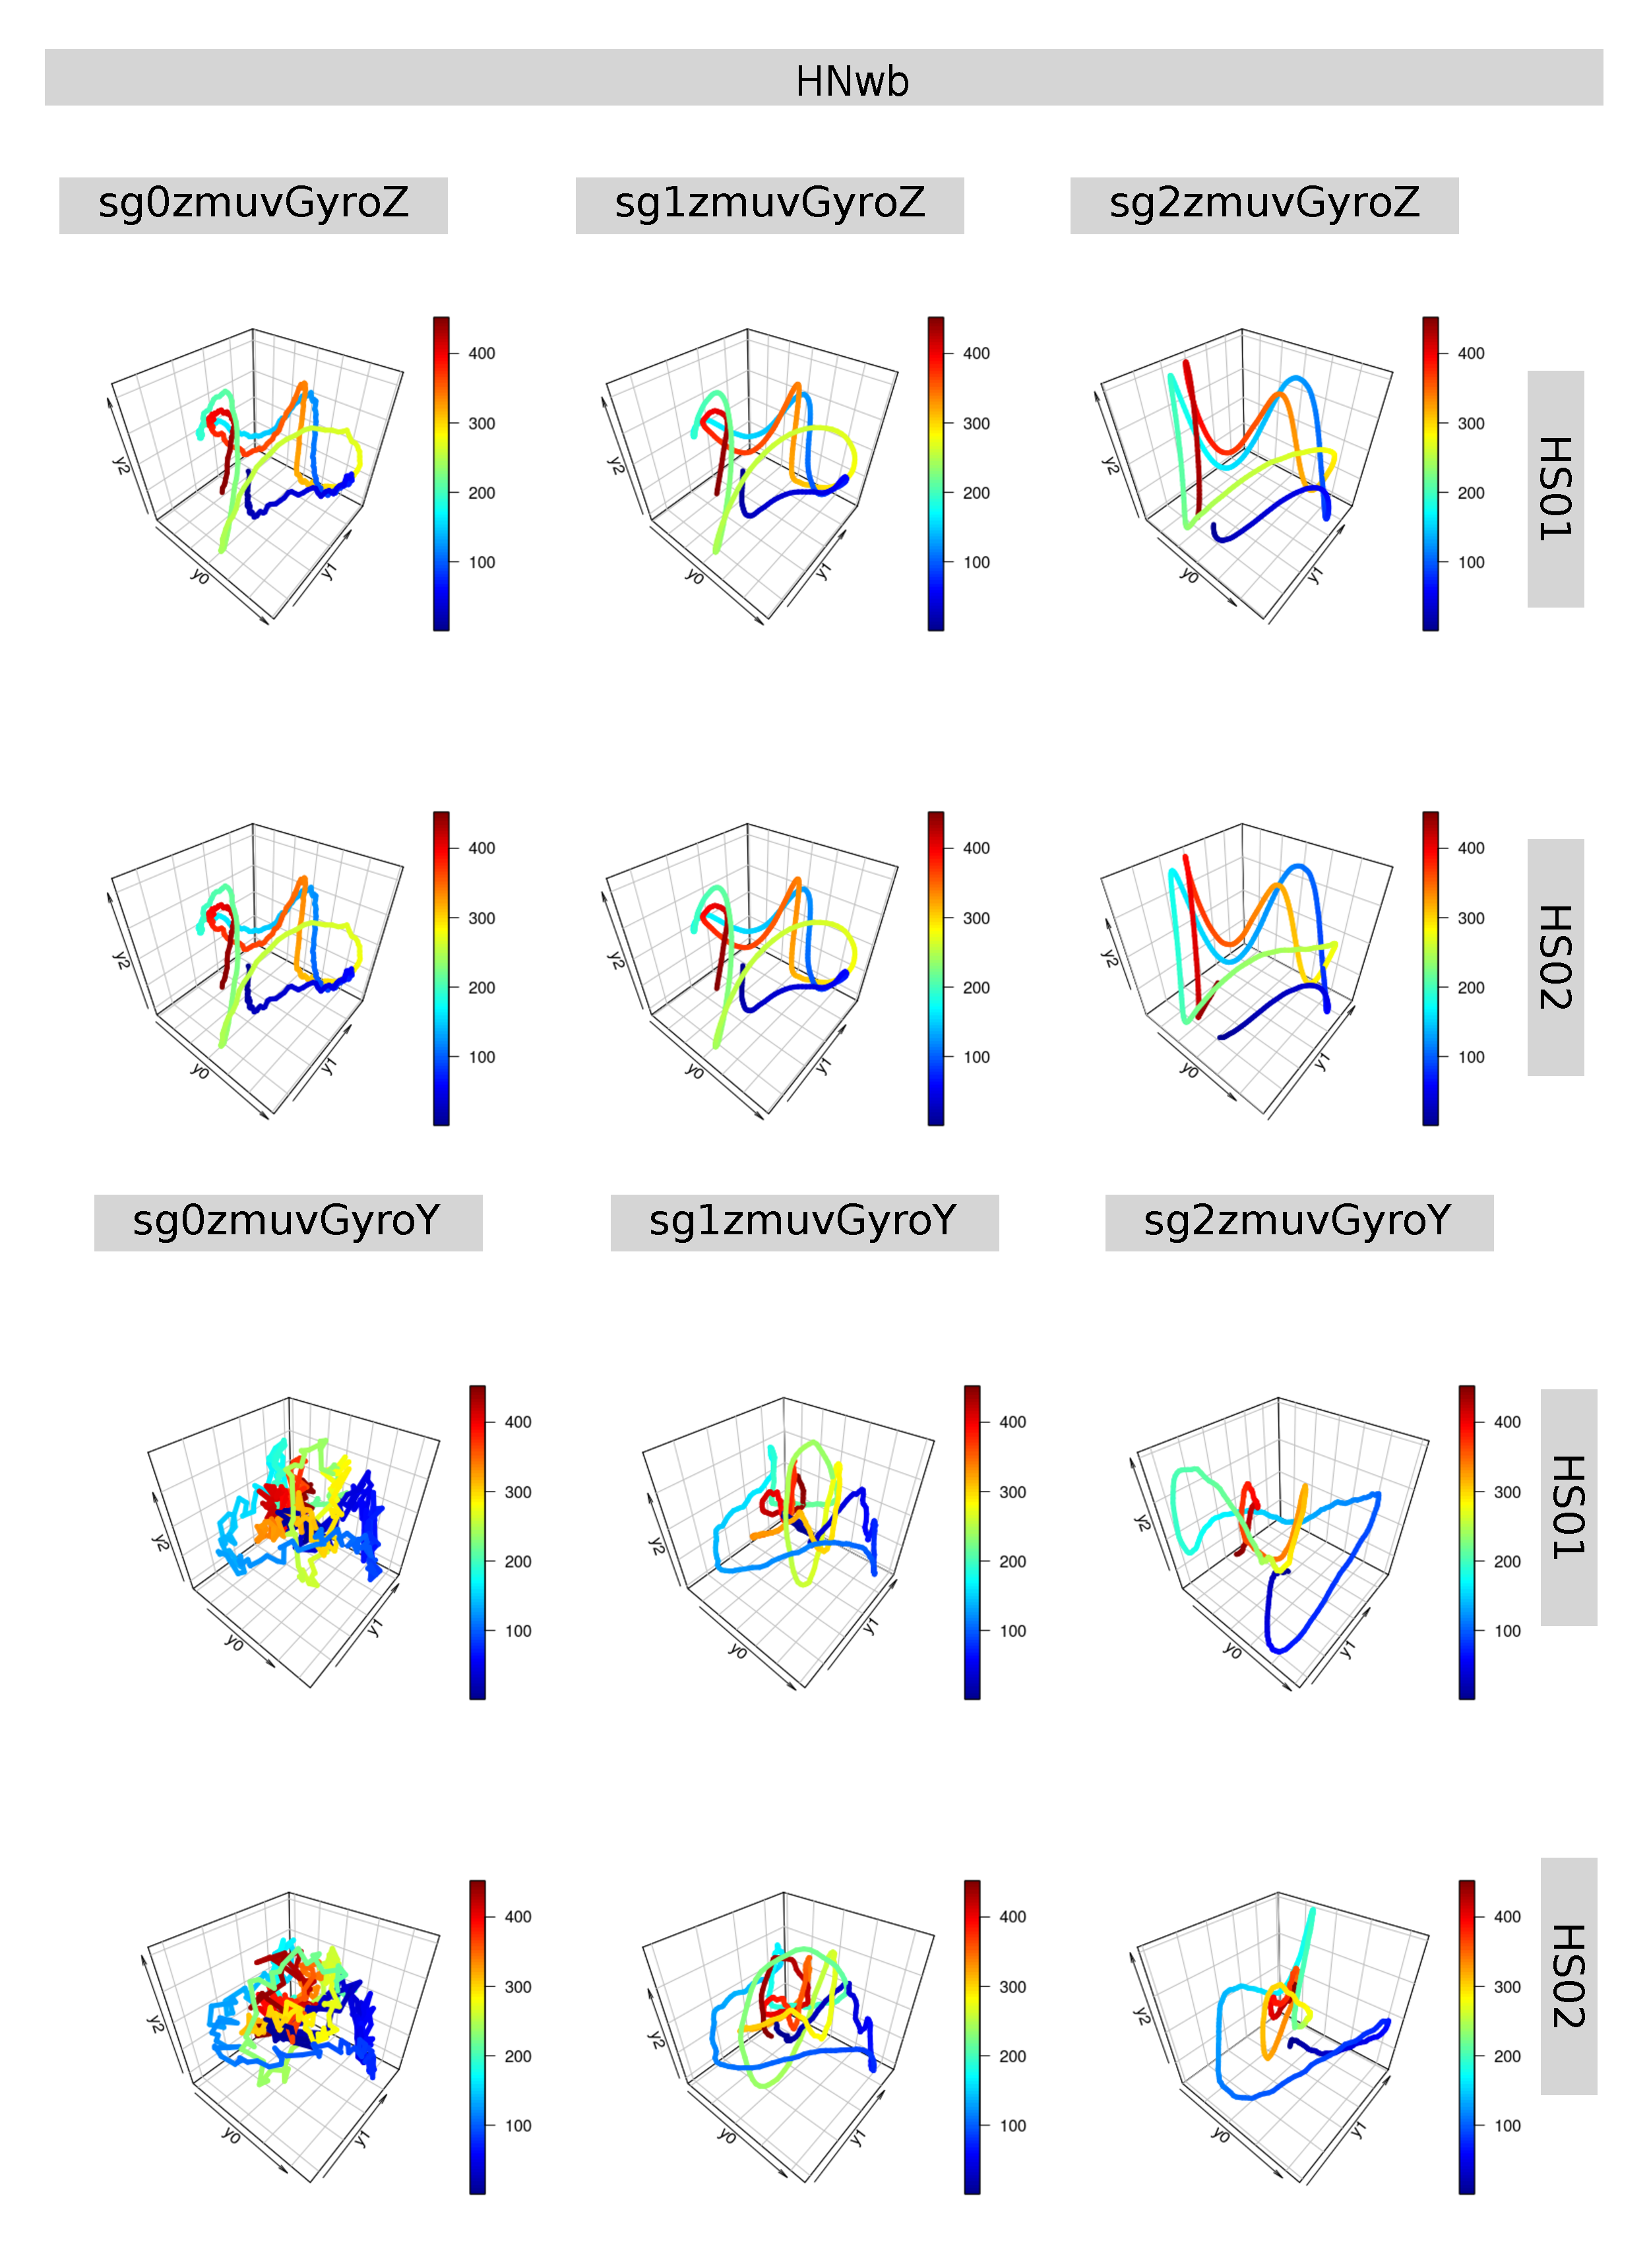
\includegraphics[height=0.8\textheight]{rss_HNwb_p04}
\caption
	[RSSs for horizontal normal arm movements (with beat)]{
	{\bf RSSs for horizontal normal arm movements (with beat).}
	Reconstructed state spaces of participant $p04$
	with time series for raw-normalised (sg0), 
	normalised-smoothed 1 (sg1) and 
	normalised-smoothed 2 (sg2), 
	with sensors attached to the participant (HS01, HS02).
	Reconstructed state spaces were computed with 
	embedding parameters $m=9$, $\tau=6$.
	R code to reproduce the figure is available from \cite{hwum2018}.
        }
     \label{fig:rss_HNwb_p04}
\end{figure}
%%---------------------------------(FIGURE)------------------------------------






%%---------------------------------(FIGURE)-------------------------------------
\begin{figure}
\centering
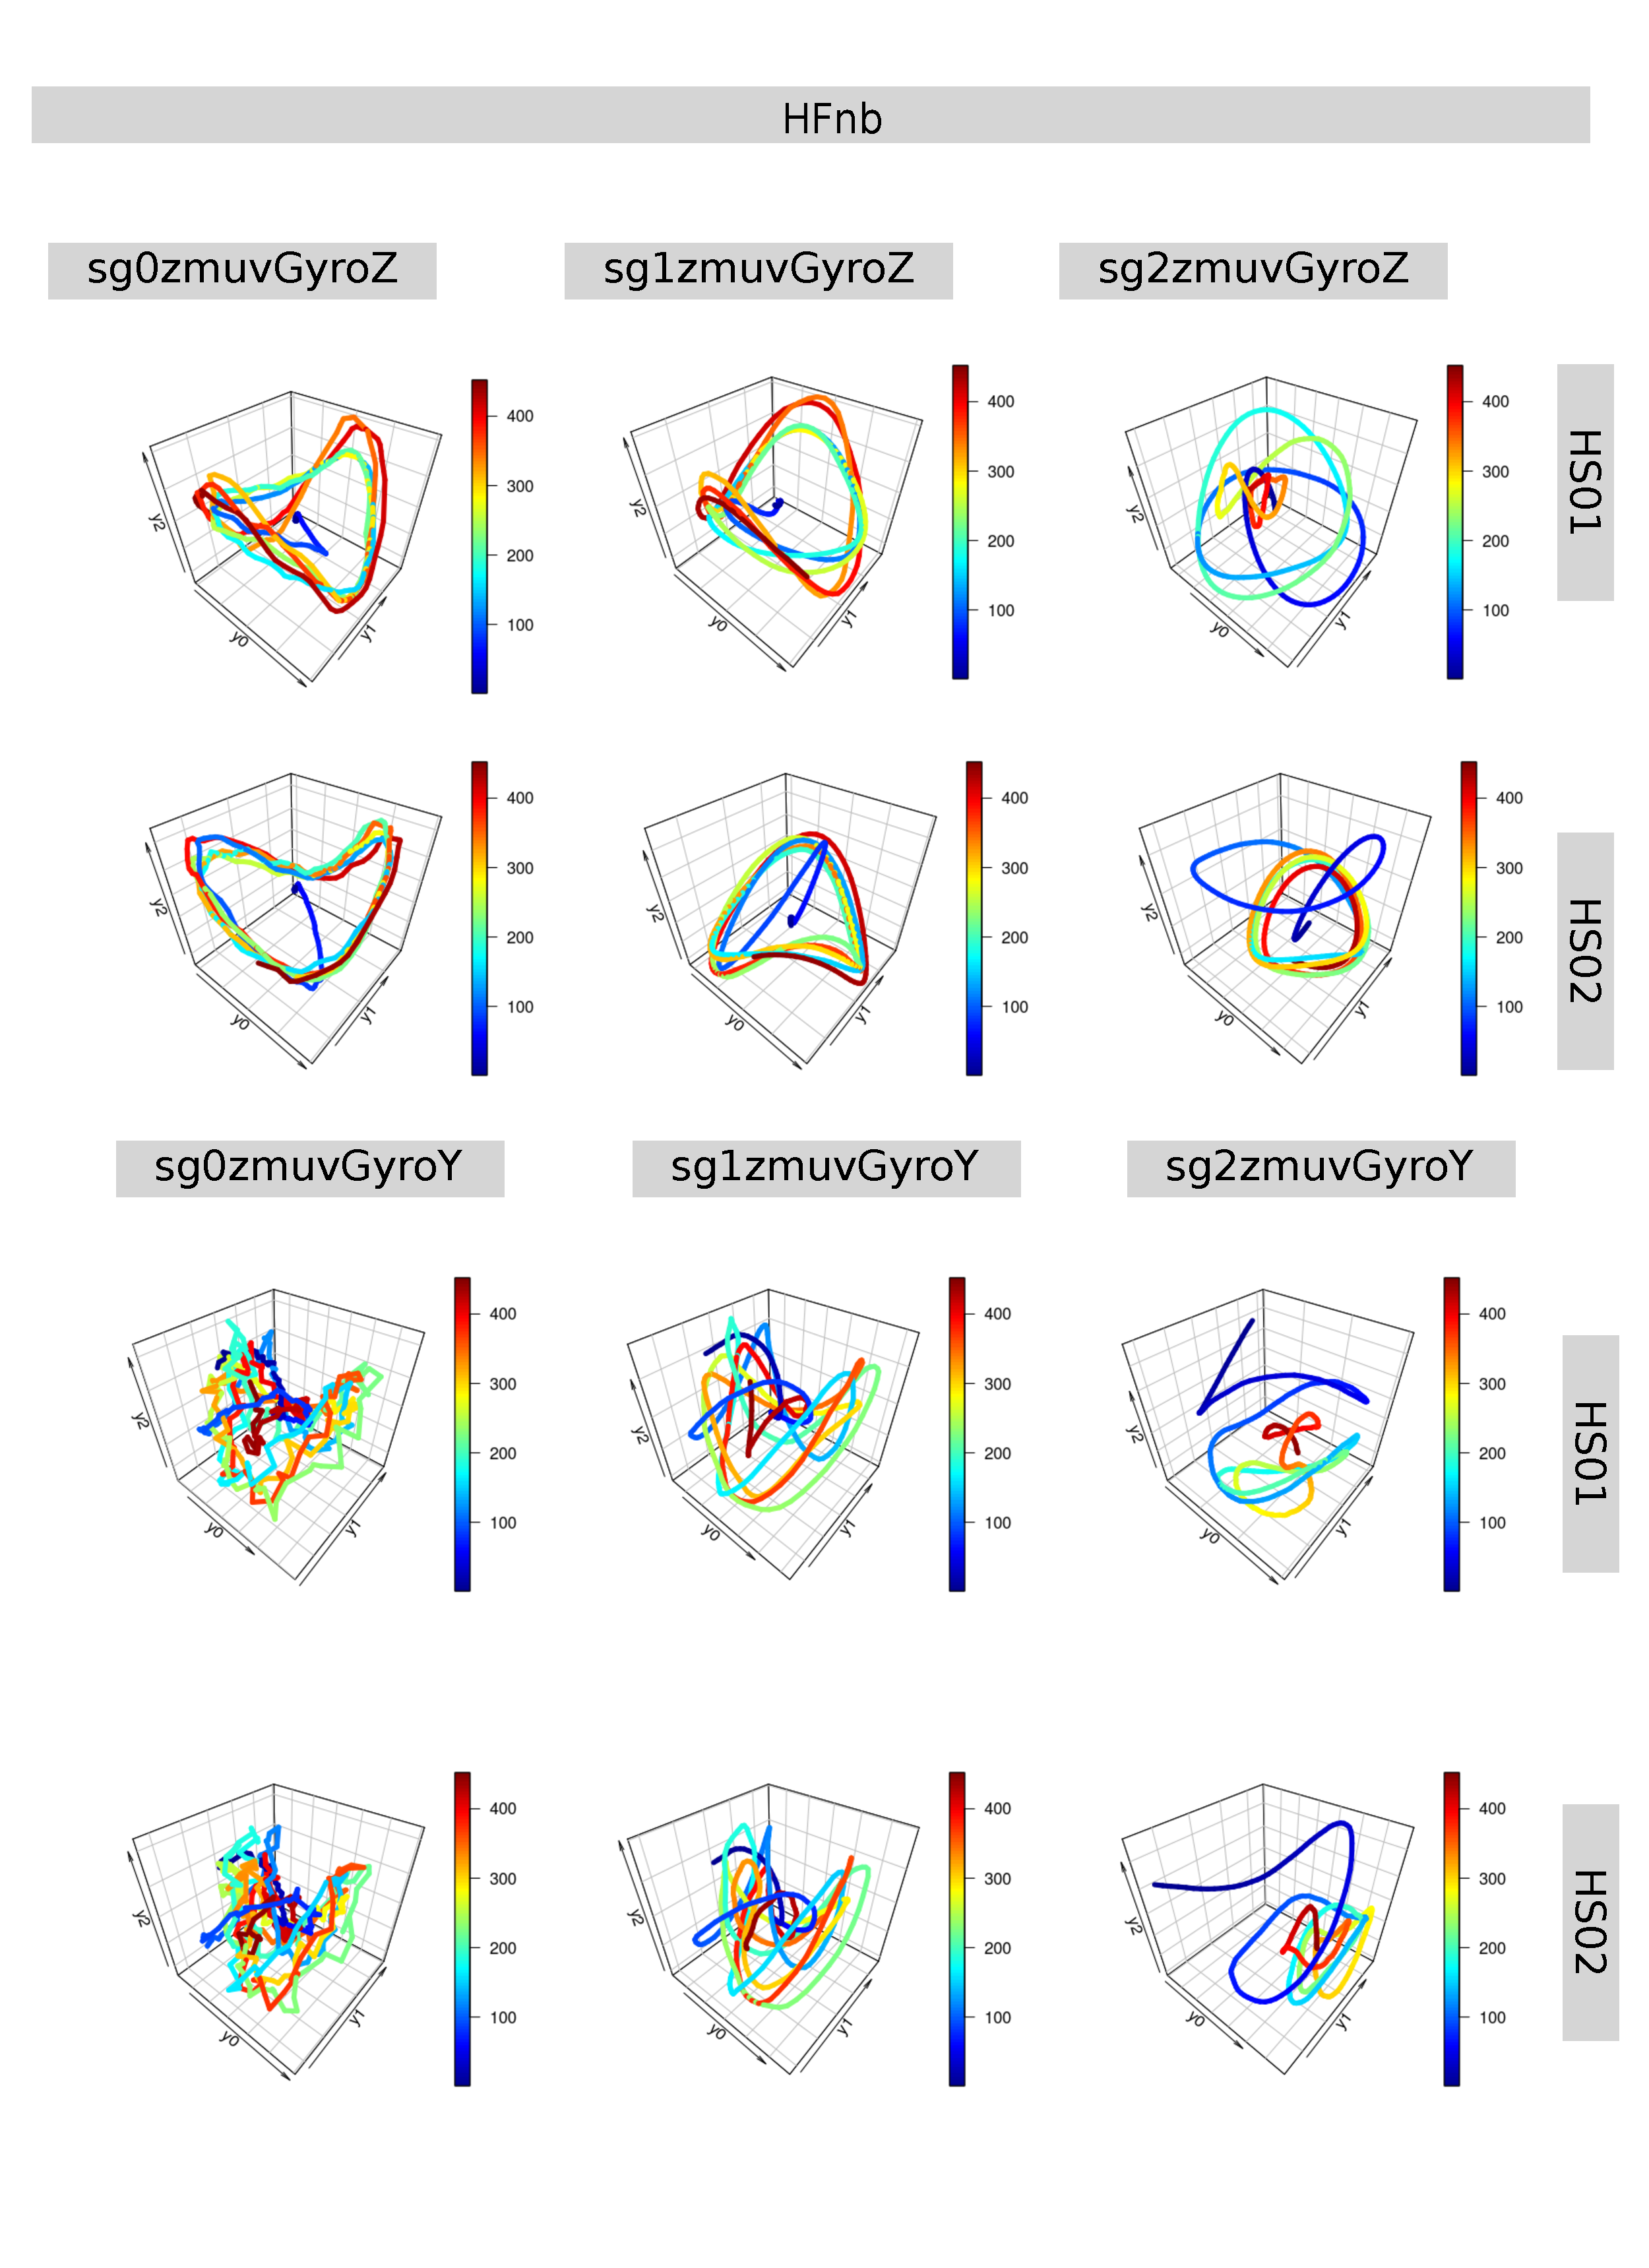
\includegraphics[height=0.8\textheight]{rss_HFnb_p04}
\caption
	[RSSs for horizontal faster arm movements (no beat)]{
	{\bf RSSs for horizontal faster arm movements (no beat).}
	Reconstructed state spaces of participant $p04$
	with time series for raw-normalised (sg0), 
	normalised-smoothed 1 (sg1) and 
	normalised-smoothed 2 (sg2), 
	with sensors attached to the participant (HS01, HS02).
	Reconstructed state spaces were computed with 
	embedding parameters $m=9$, $\tau=6$.
	R code to reproduce the figure is available from \cite{hwum2018}.
        }
     \label{fig:rss_HFnb_p04}
\end{figure}
%%---------------------------------(FIGURE)------------------------------------



%%---------------------------------(FIGURE)-------------------------------------
\begin{figure}
\centering
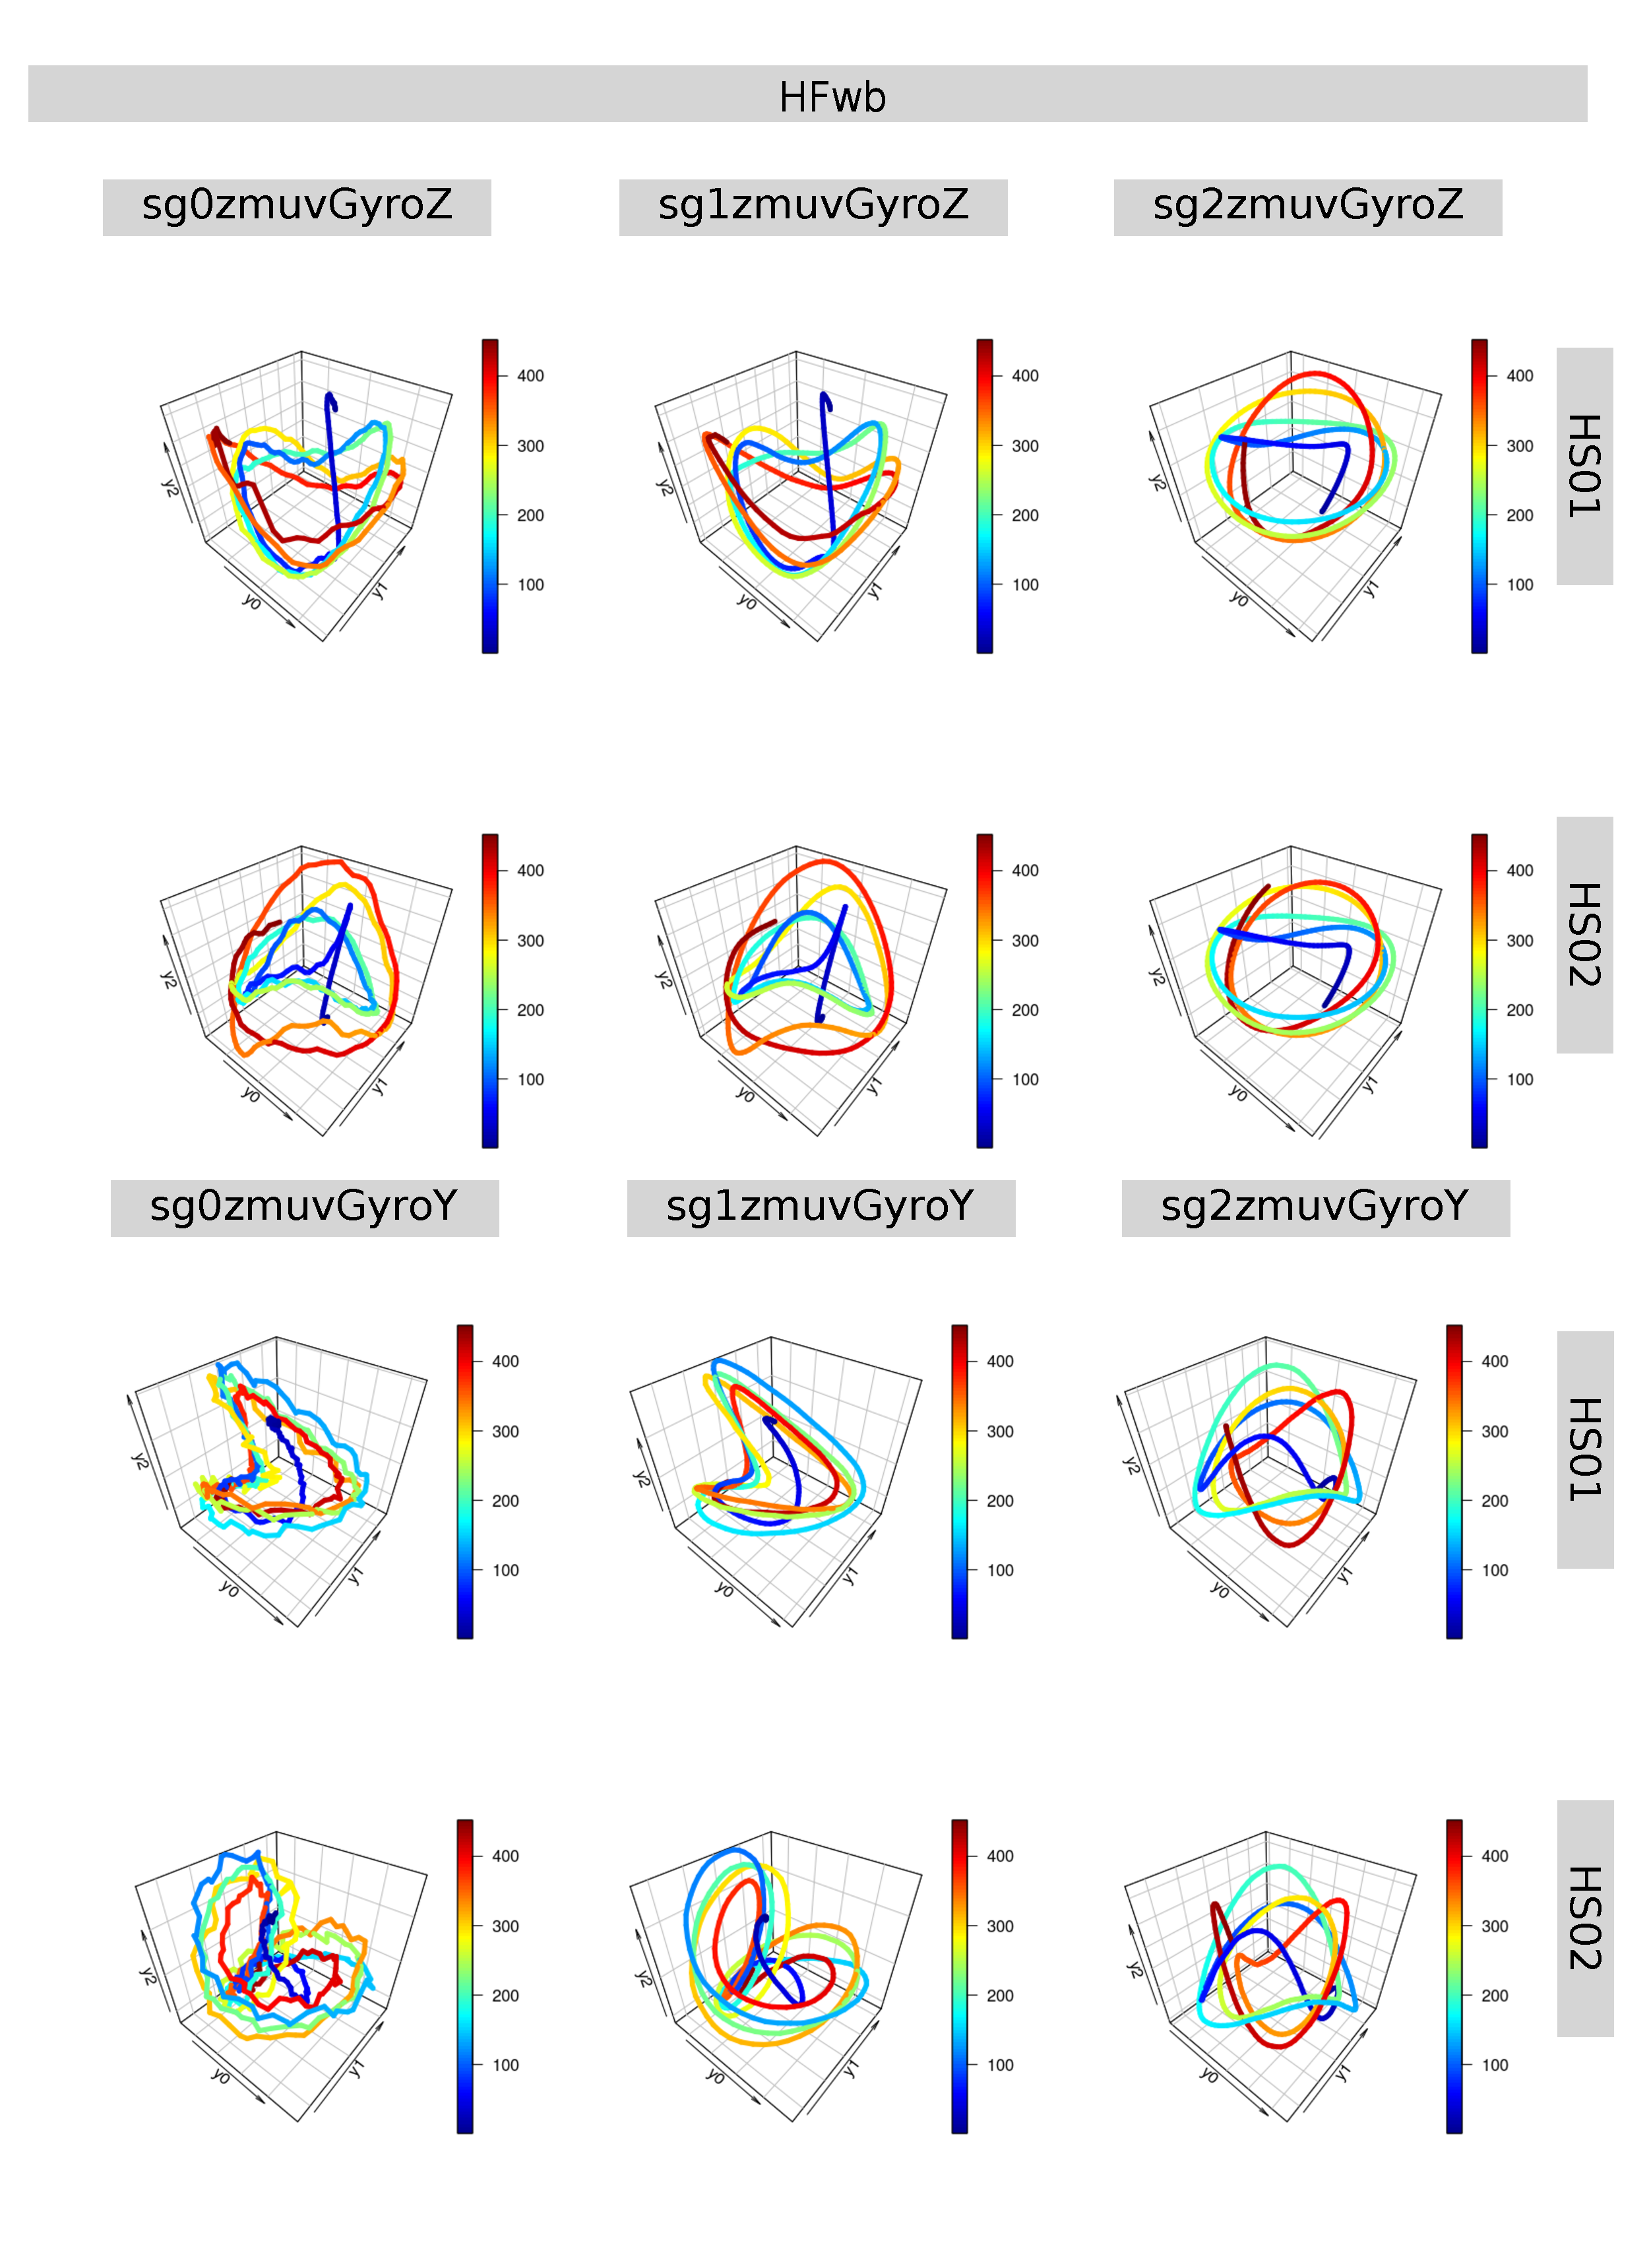
\includegraphics[height=0.8\textheight]{rss_HFwb_p04}
\caption
	[RSSs for horizontal faster arm movements (with beat)]{
	{\bf RSSs for horizontal faster arm movements (with beat).}
	Reconstructed state spaces of participant $p04$
	with time series for raw-normalised (sg0), 
	normalised-smoothed 1 (sg1) and 
	normalised-smoothed 2 (sg2), 
	with sensors attached to the participant (HS01, HS02).
	Reconstructed state spaces were computed with 
	embedding parameters $m=9$, $\tau=6$.
	R code to reproduce the figure is available from \cite{hwum2018}.
        }
     \label{fig:rss_HFwb_p04}
\end{figure}
%%---------------------------------(FIGURE)------------------------------------




%%%%%%%%%VERTICAL


%%---------------------------------(FIGURE)-------------------------------------
\begin{figure}
\centering
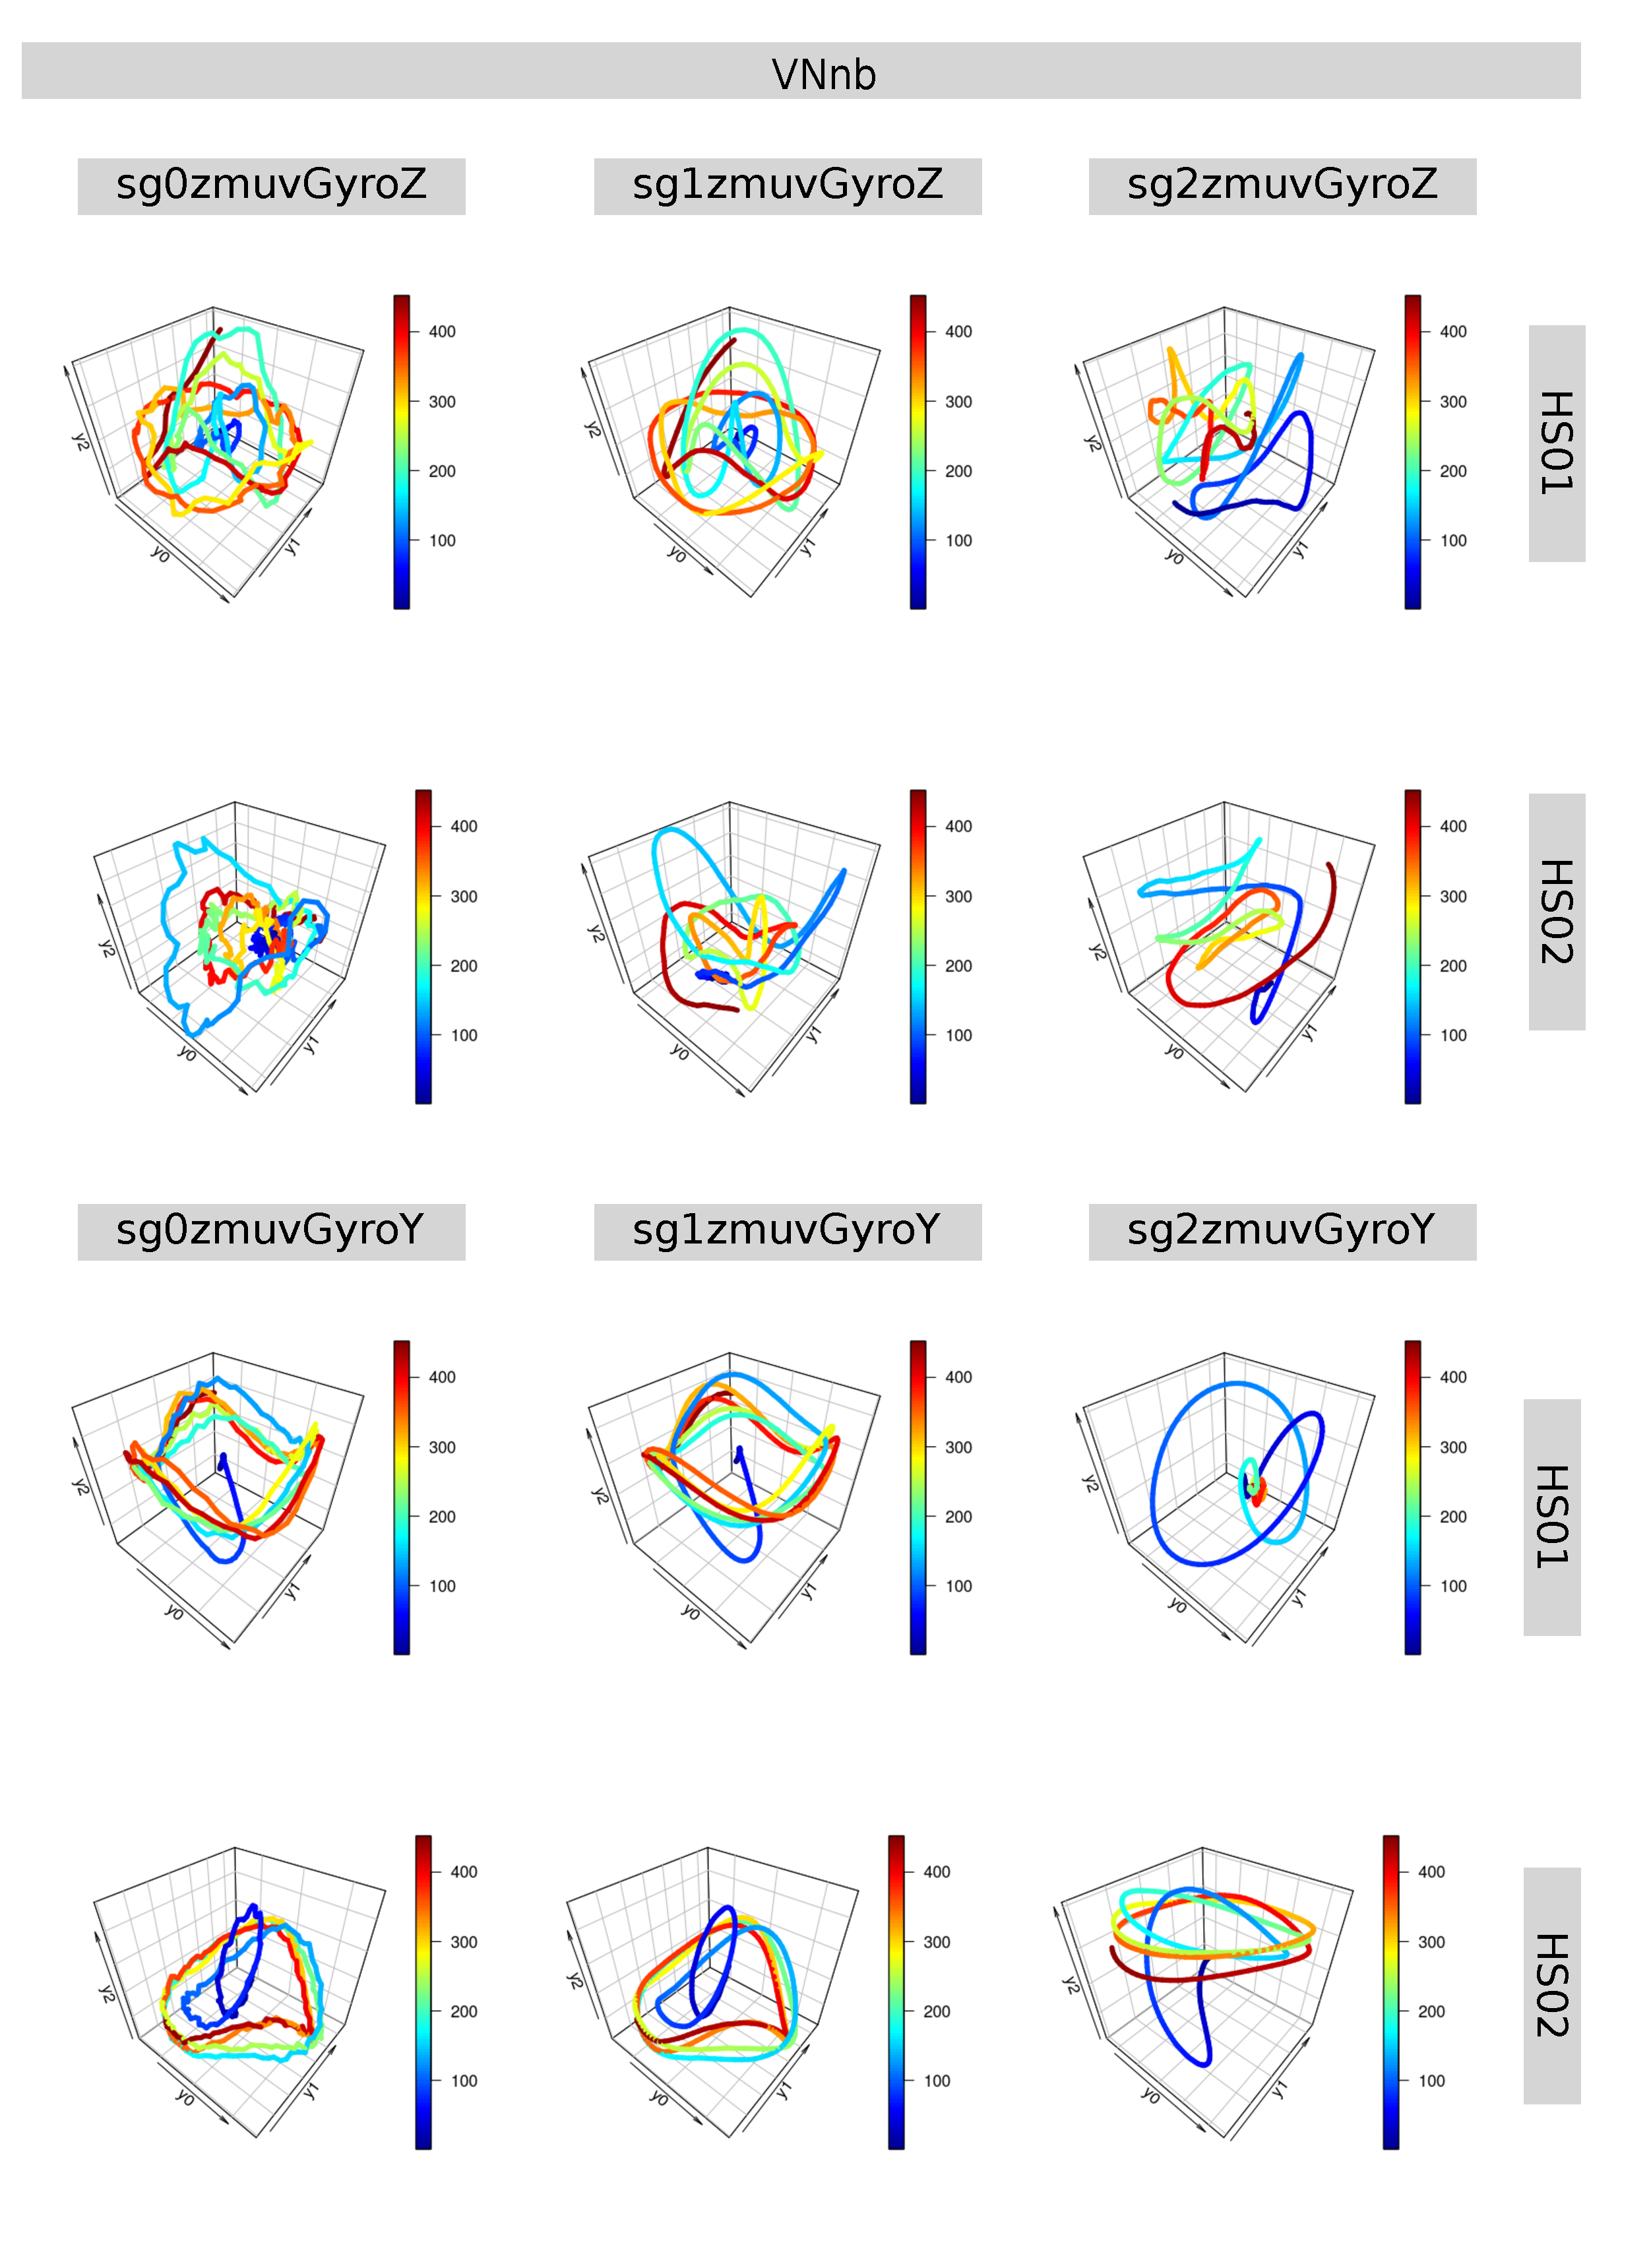
\includegraphics[height=0.8\textheight]{rss_VNnb_p04}
\caption
	[RSSs for vertical normal arm movements (no beat)]{
	{\bf RSSs for vertical normal arm movements (no beat).}
	Reconstructed state spaces of participant $p04$
	with time series for raw-normalised (sg0), 
	normalised-smoothed 1 (sg1) and 
	normalised-smoothed 2 (sg2), 
	with sensors attached to the participant (HS01, HS02).
	Reconstructed state spaces were computed with 
	embedding parameters $m=9$, $\tau=6$.
	R code to reproduce the figure is available from \cite{hwum2018}.
        }
     \label{fig:rss_VNnb_p04}
\end{figure}
%%---------------------------------(FIGURE)------------------------------------



%%---------------------------------(FIGURE)-------------------------------------
\begin{figure}
\centering
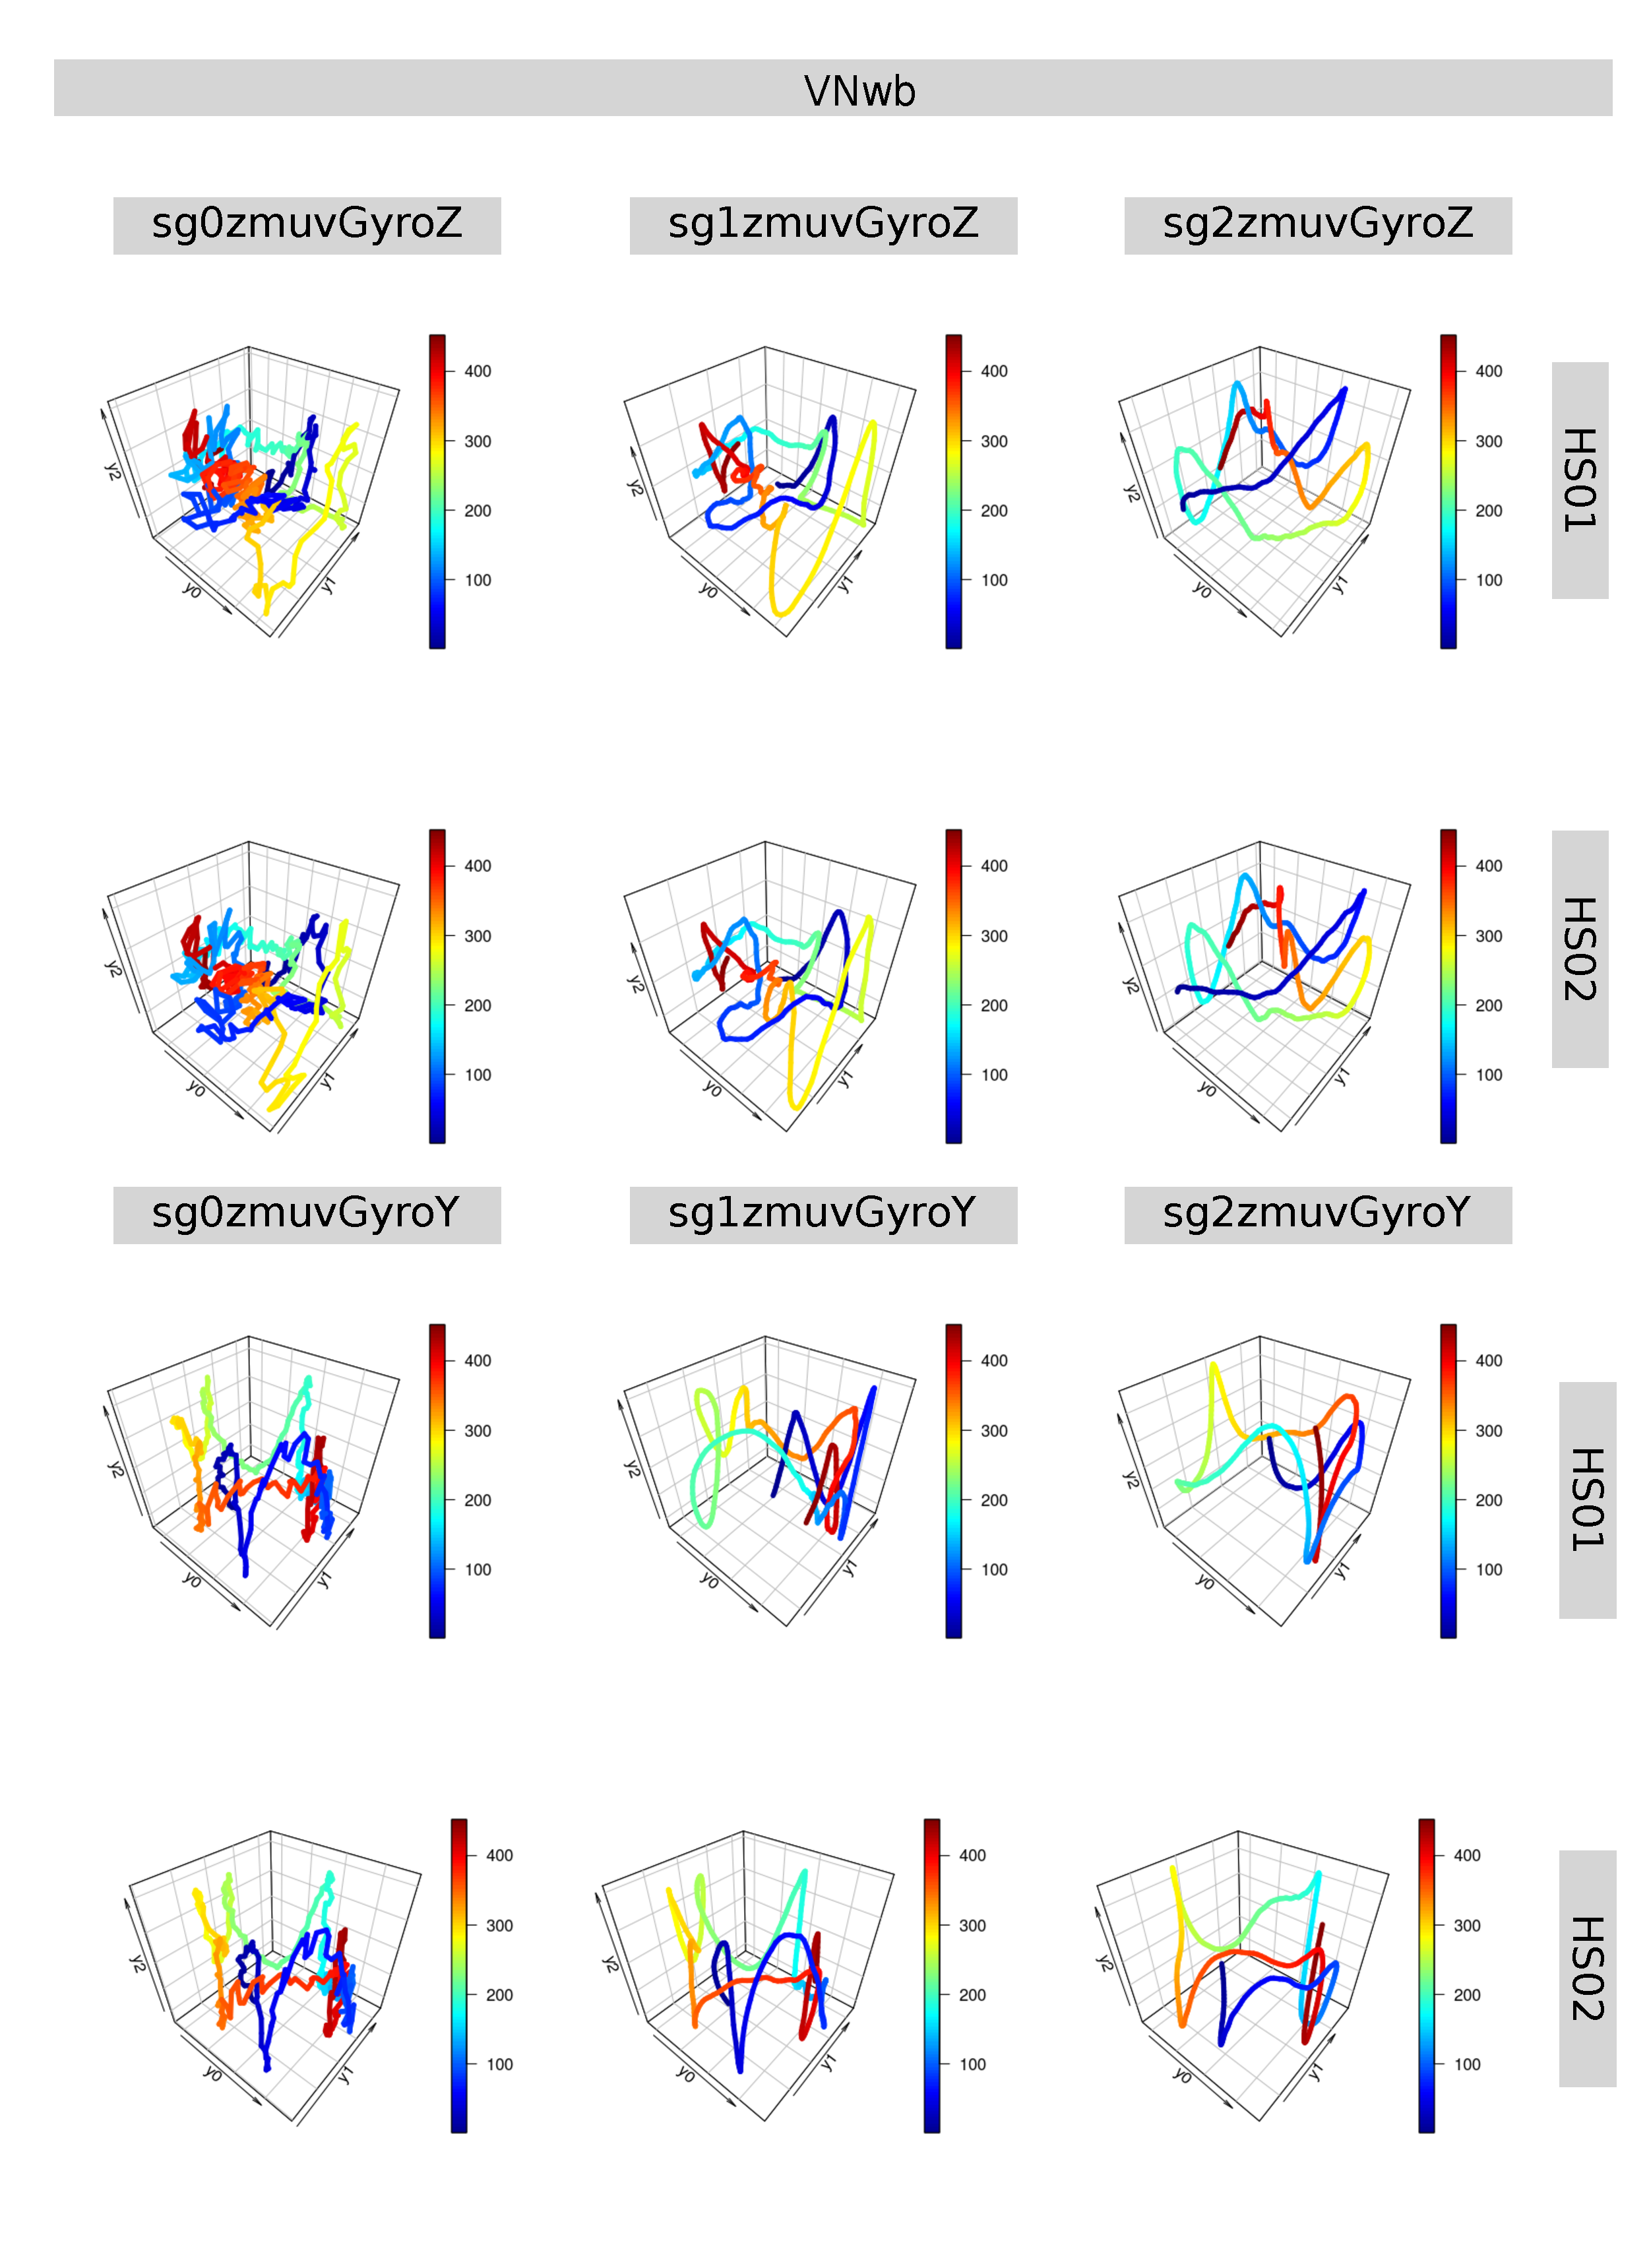
\includegraphics[height=0.8\textheight]{rss_VNwb_p04}
\caption
	[RSSs for vertical normal arm movements (with beat)]{
	{\bf RSSs for vertical normal arm movements (with beat).}
	Reconstructed state spaces of participant $p04$
	with time series for raw-normalised (sg0), 
	normalised-smoothed 1 (sg1) and 
	normalised-smoothed 2 (sg2), 
	with sensors attached to the participant (HS01, HS02).
	Reconstructed state spaces were computed with 
	embedding parameters $m=9$, $\tau=6$.
	R code to reproduce the figure is available from \cite{hwum2018}.
        }
     \label{fig:rss_VNwb_p04}
\end{figure}
%%---------------------------------(FIGURE)------------------------------------






%%---------------------------------(FIGURE)-------------------------------------
\begin{figure}
\centering
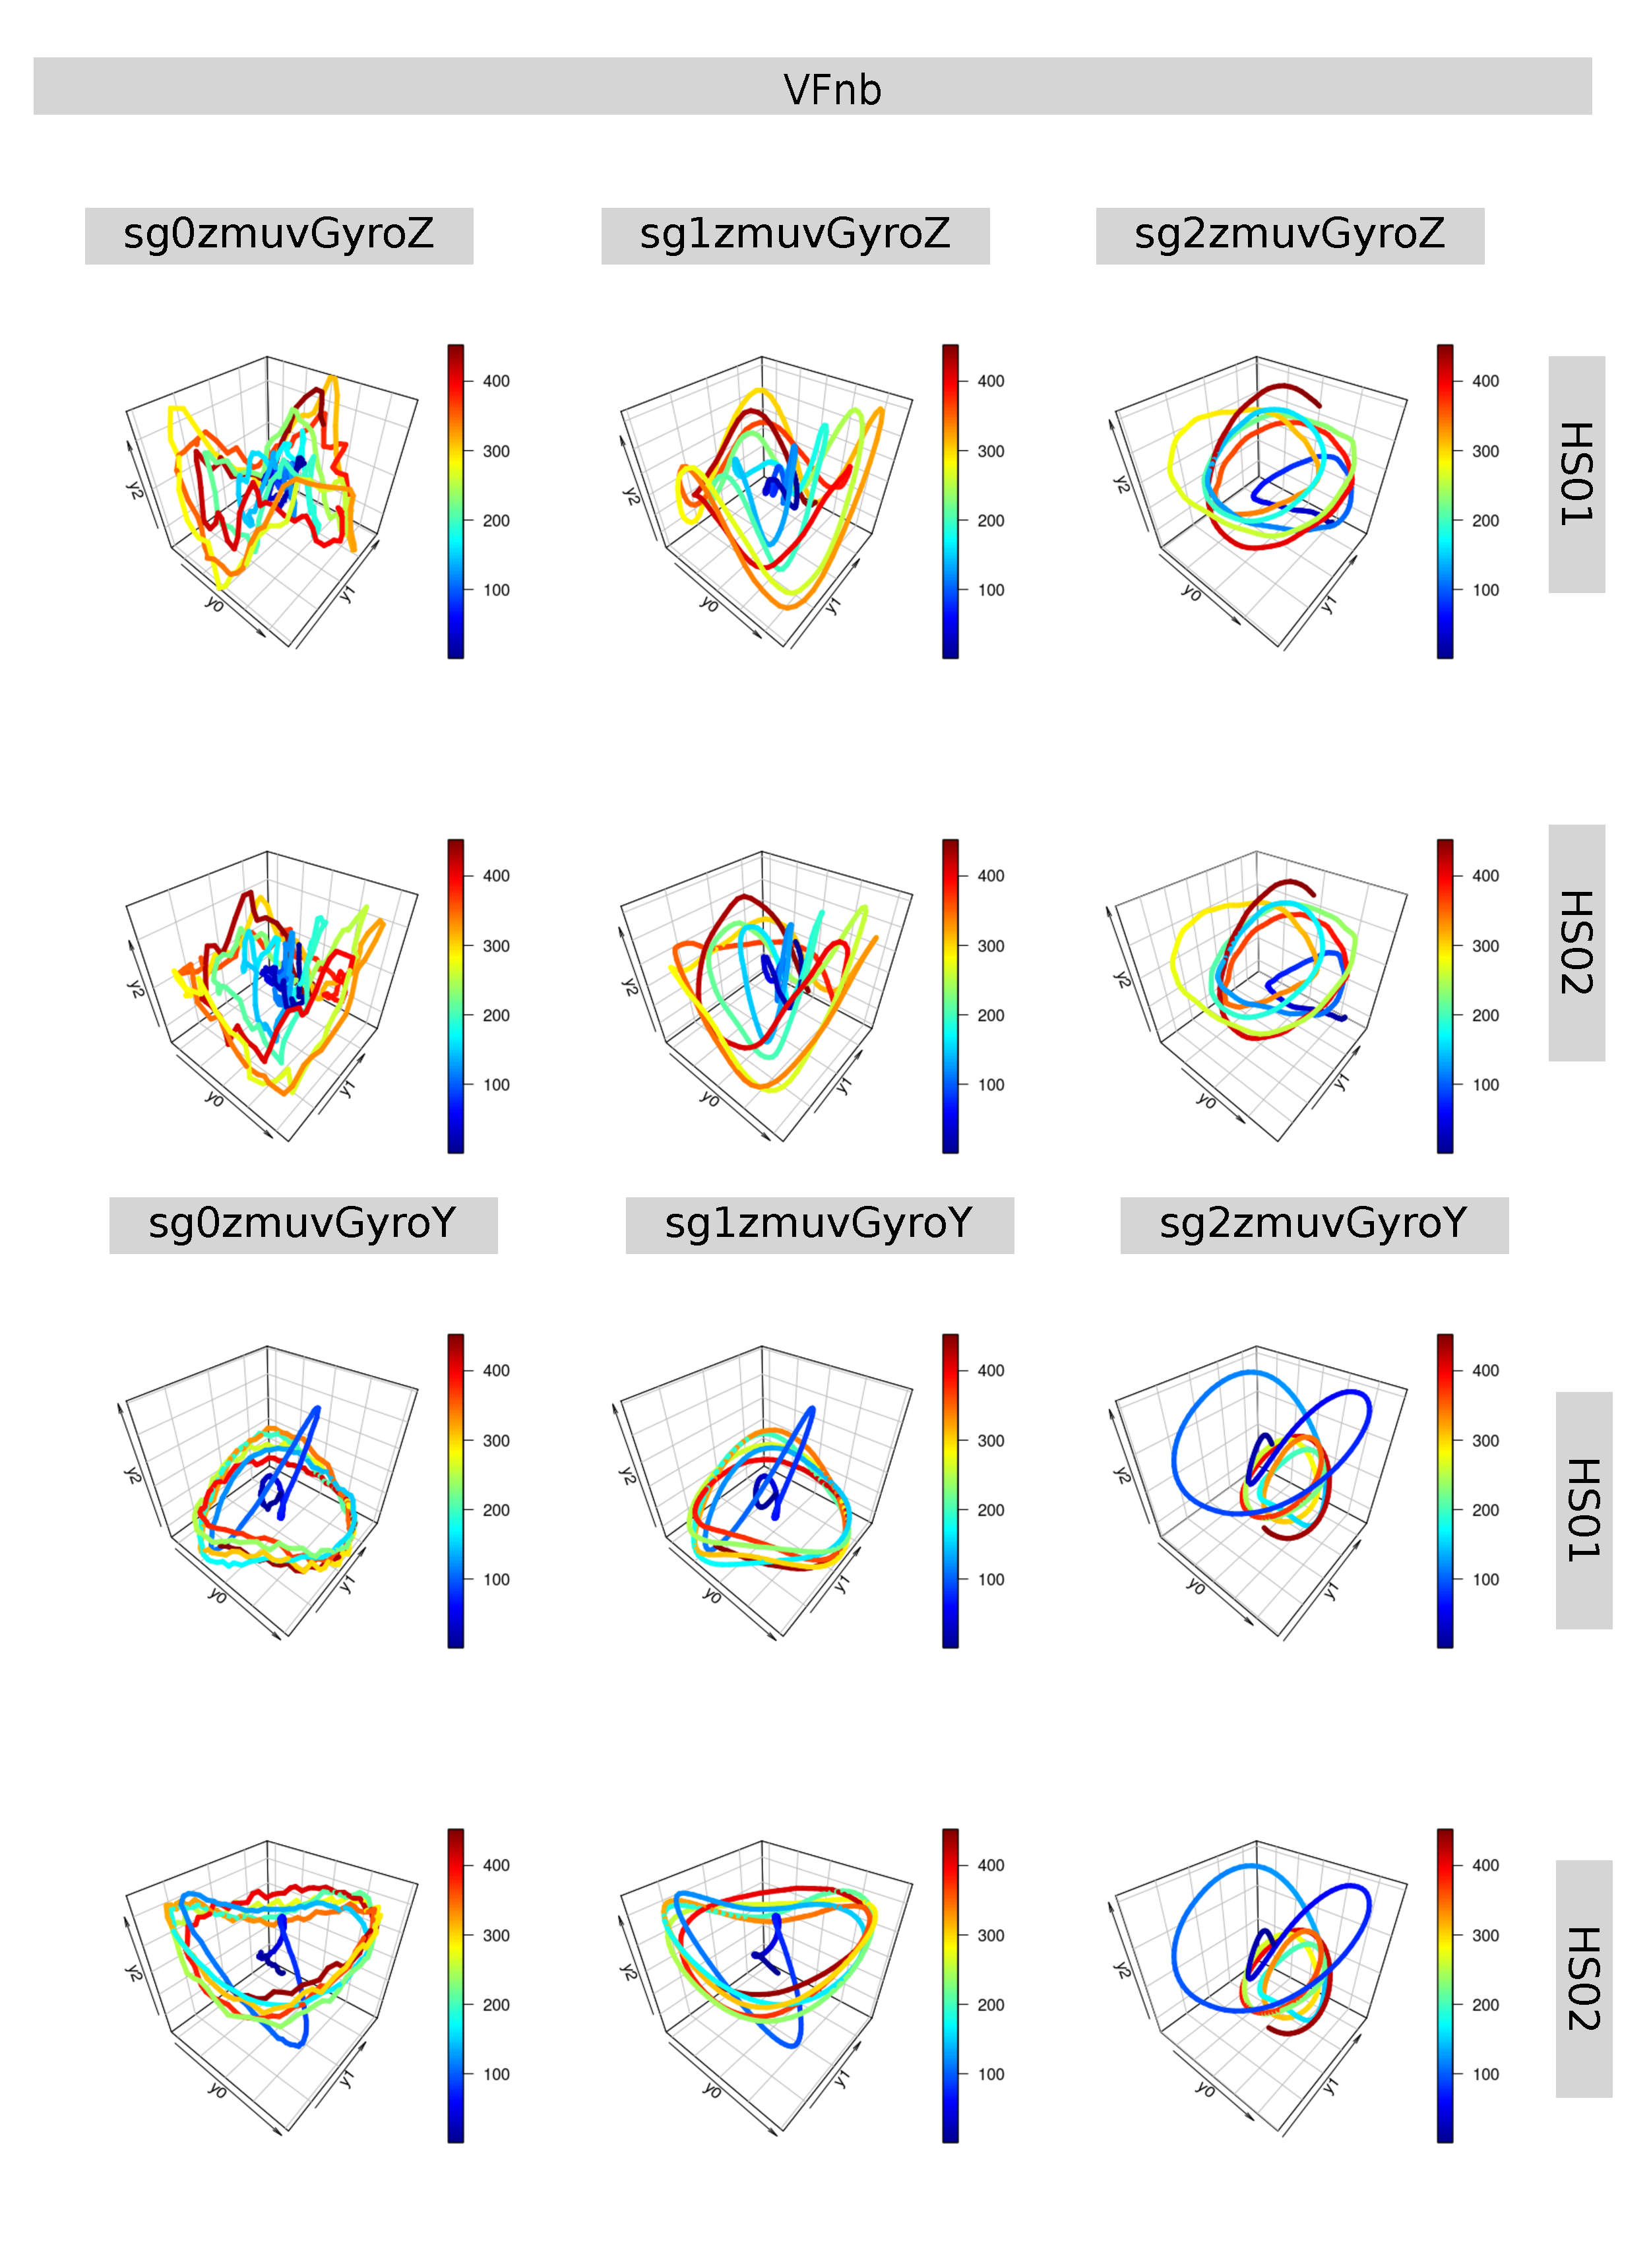
\includegraphics[height=0.8\textheight]{rss_VFnb_p04}
\caption
	[RSSs for vertical faster arm movements (no beat)]{
	{\bf RSSs for vertical faster arm movements (no beat).}
	Reconstructed state spaces of participant $p04$
	with time series for raw-normalised (sg0), 
	normalised-smoothed 1 (sg1) and 
	normalised-smoothed 2 (sg2), 
	with sensors attached to the participant (HS01, HS02).
	Reconstructed state spaces were computed with 
	embedding parameters $m=9$, $\tau=6$.
	R code to reproduce the figure is available from \cite{hwum2018}.
        }
     \label{fig:rss_VFnb_p04}
\end{figure}
%%---------------------------------(FIGURE)------------------------------------



%%---------------------------------(FIGURE)-------------------------------------
\begin{figure}
\centering
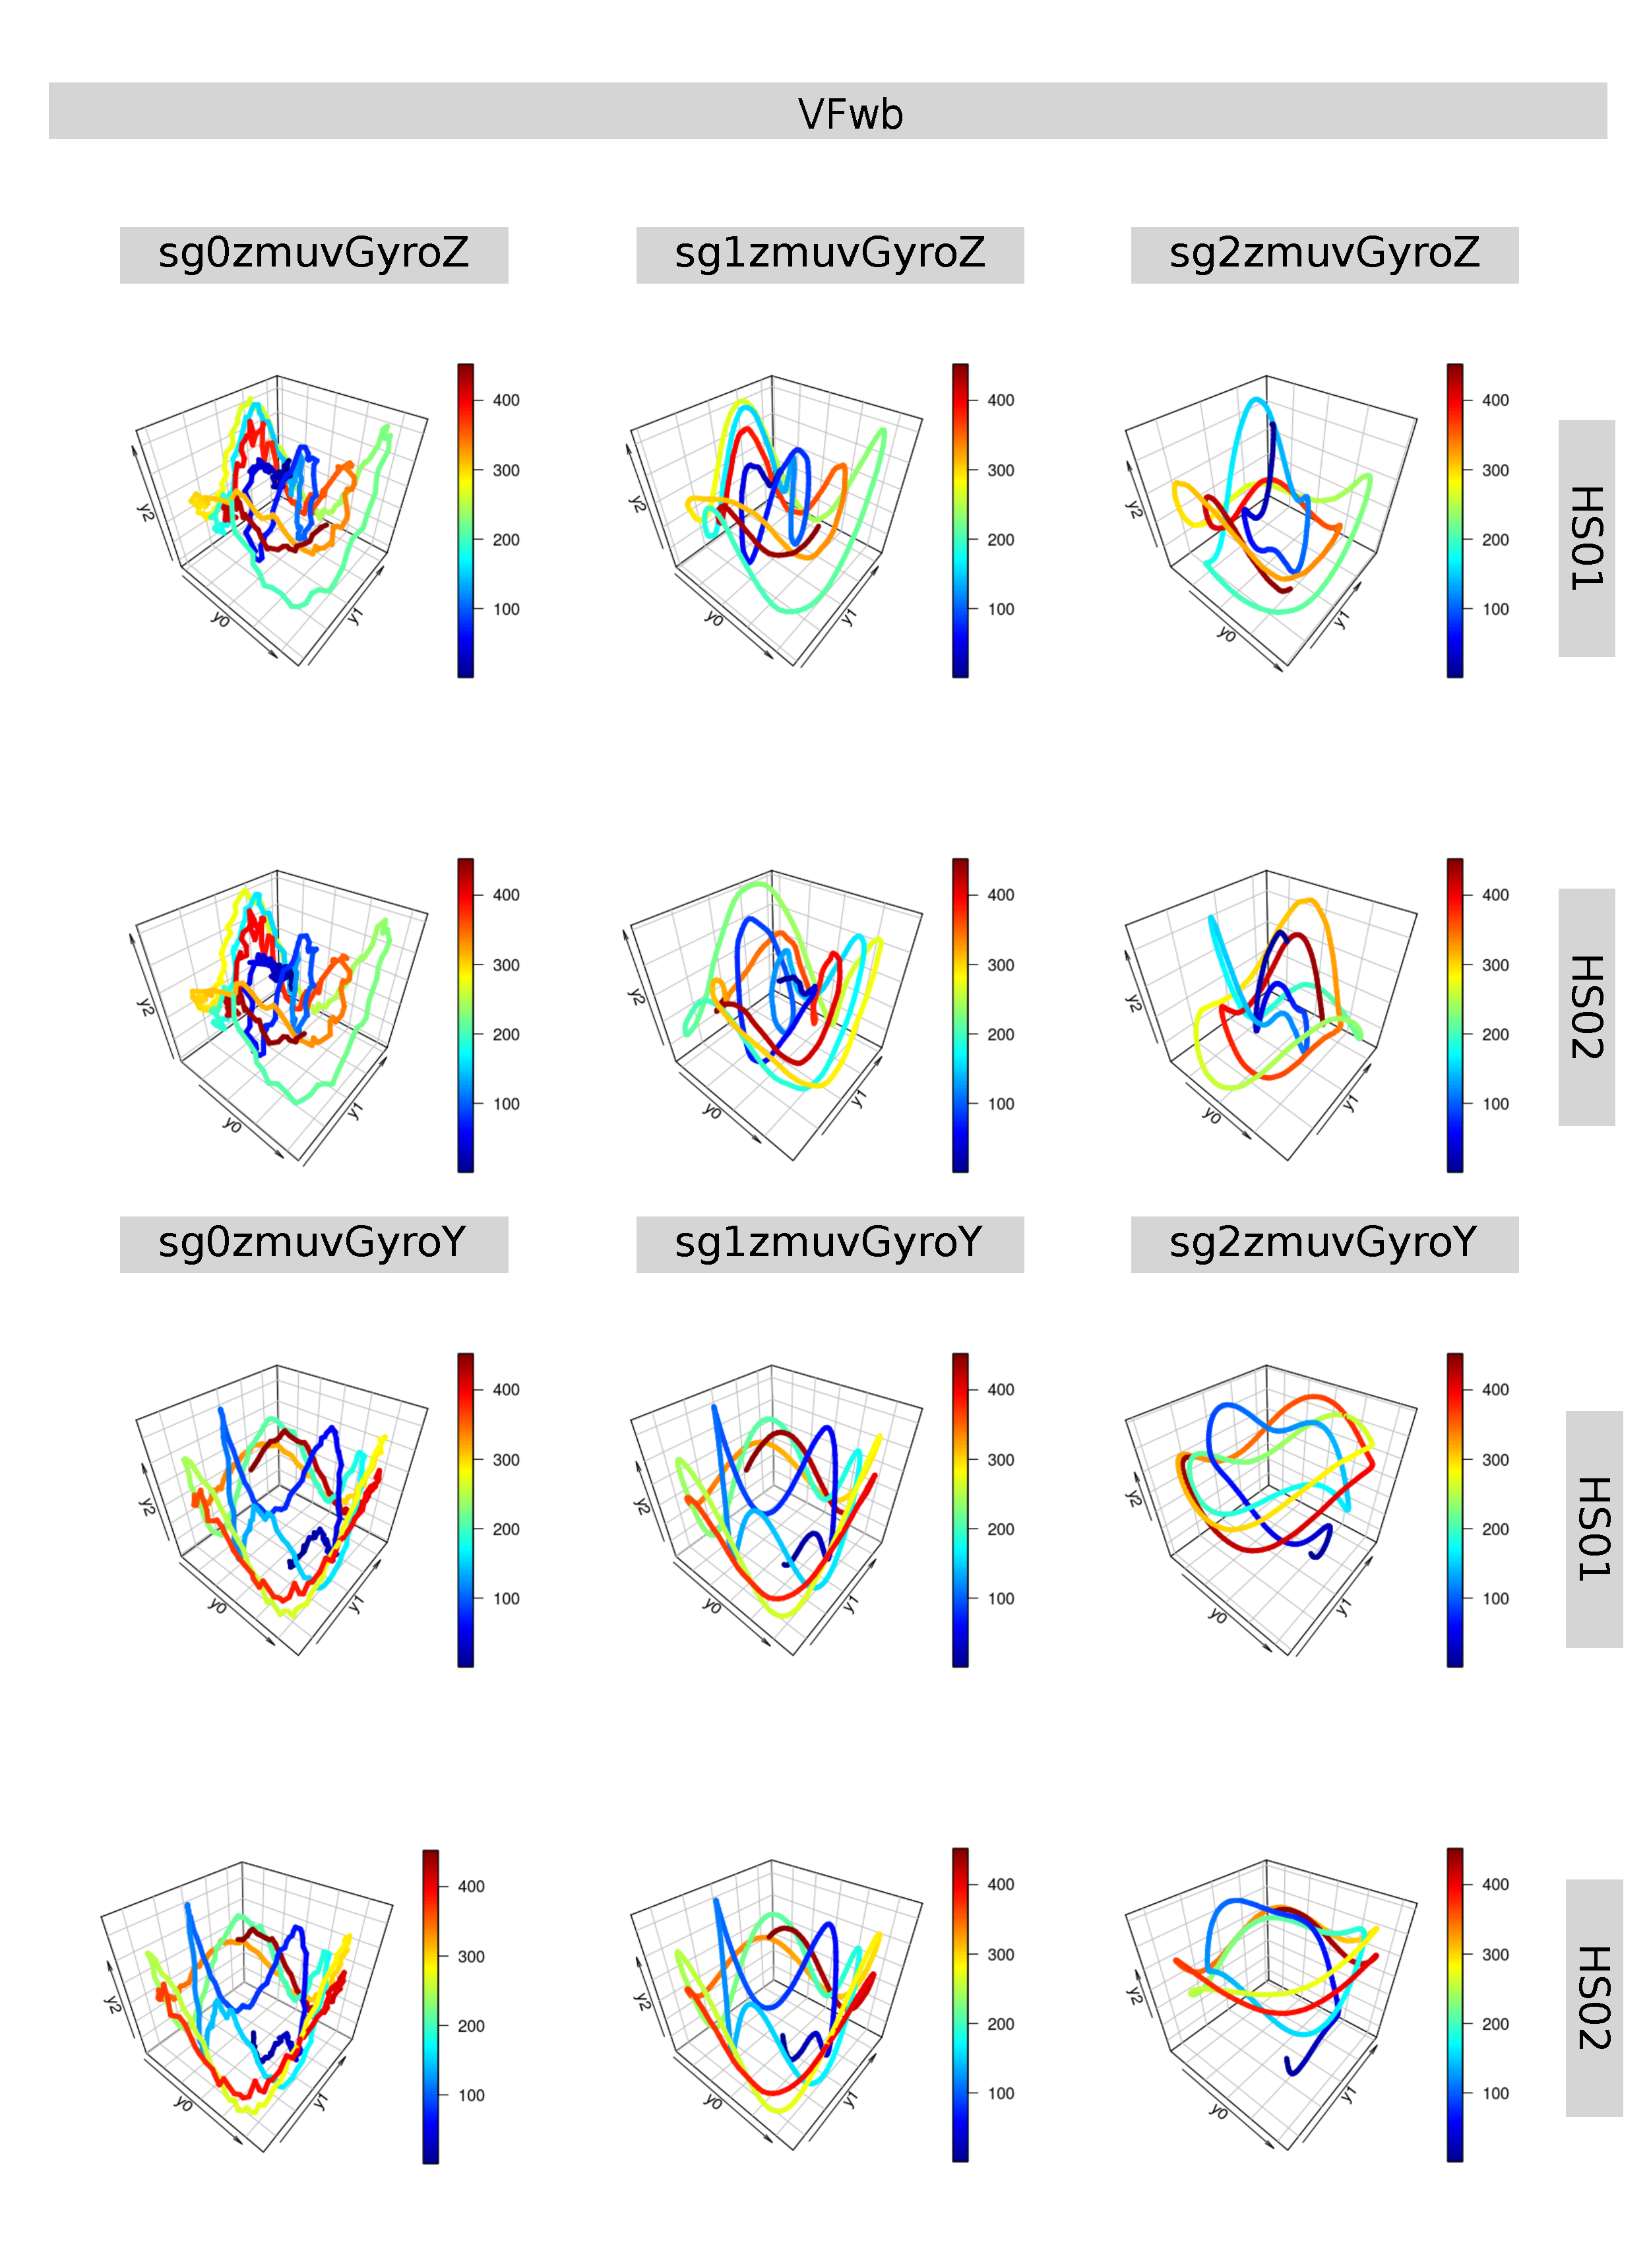
\includegraphics[height=0.8\textheight]{rss_VFwb_p04}
\caption
	[RSSs for vertical faster arm movements (with beat)]{
	{\bf RSSs for vertical faster arm movements (with beat).}
	Reconstructed state spaces of participant $p04$
	with time series for raw-normalised (sg0), 
	normalised-smoothed 1 (sg1) and 
	normalised-smoothed 2 (sg2), 
	with sensors attached to the participant (HS01, HS02).
	Reconstructed state spaces were computed with 
	embedding parameters $m=9$, $\tau=6$.
	R code to reproduce the figure is available from \cite{hwum2018}.
        }
     \label{fig:rss_VFwb_p04}
\end{figure}
%%---------------------------------(FIGURE)------------------------------------






\newpage
\section{RPs} \label{appendix:d:rps}


The following Figs.  
\ref{fig:rps_HF_w500_p04},
\ref{fig:rps_HN_w500_p04},
\ref{fig:rps_VF_w500_p04},
\ref{fig:rps_VN_w500_p04}
illustrate reconstructed state spaces 
of participant $p04$ with a window length size of 500 samples.
We refer the reader to download the data and code at \cite{hwum2018}
for the remained window size lengths and other participants.






%%---------------------------------(FIGURE)------------------------------------
\begin{figure}
\centering
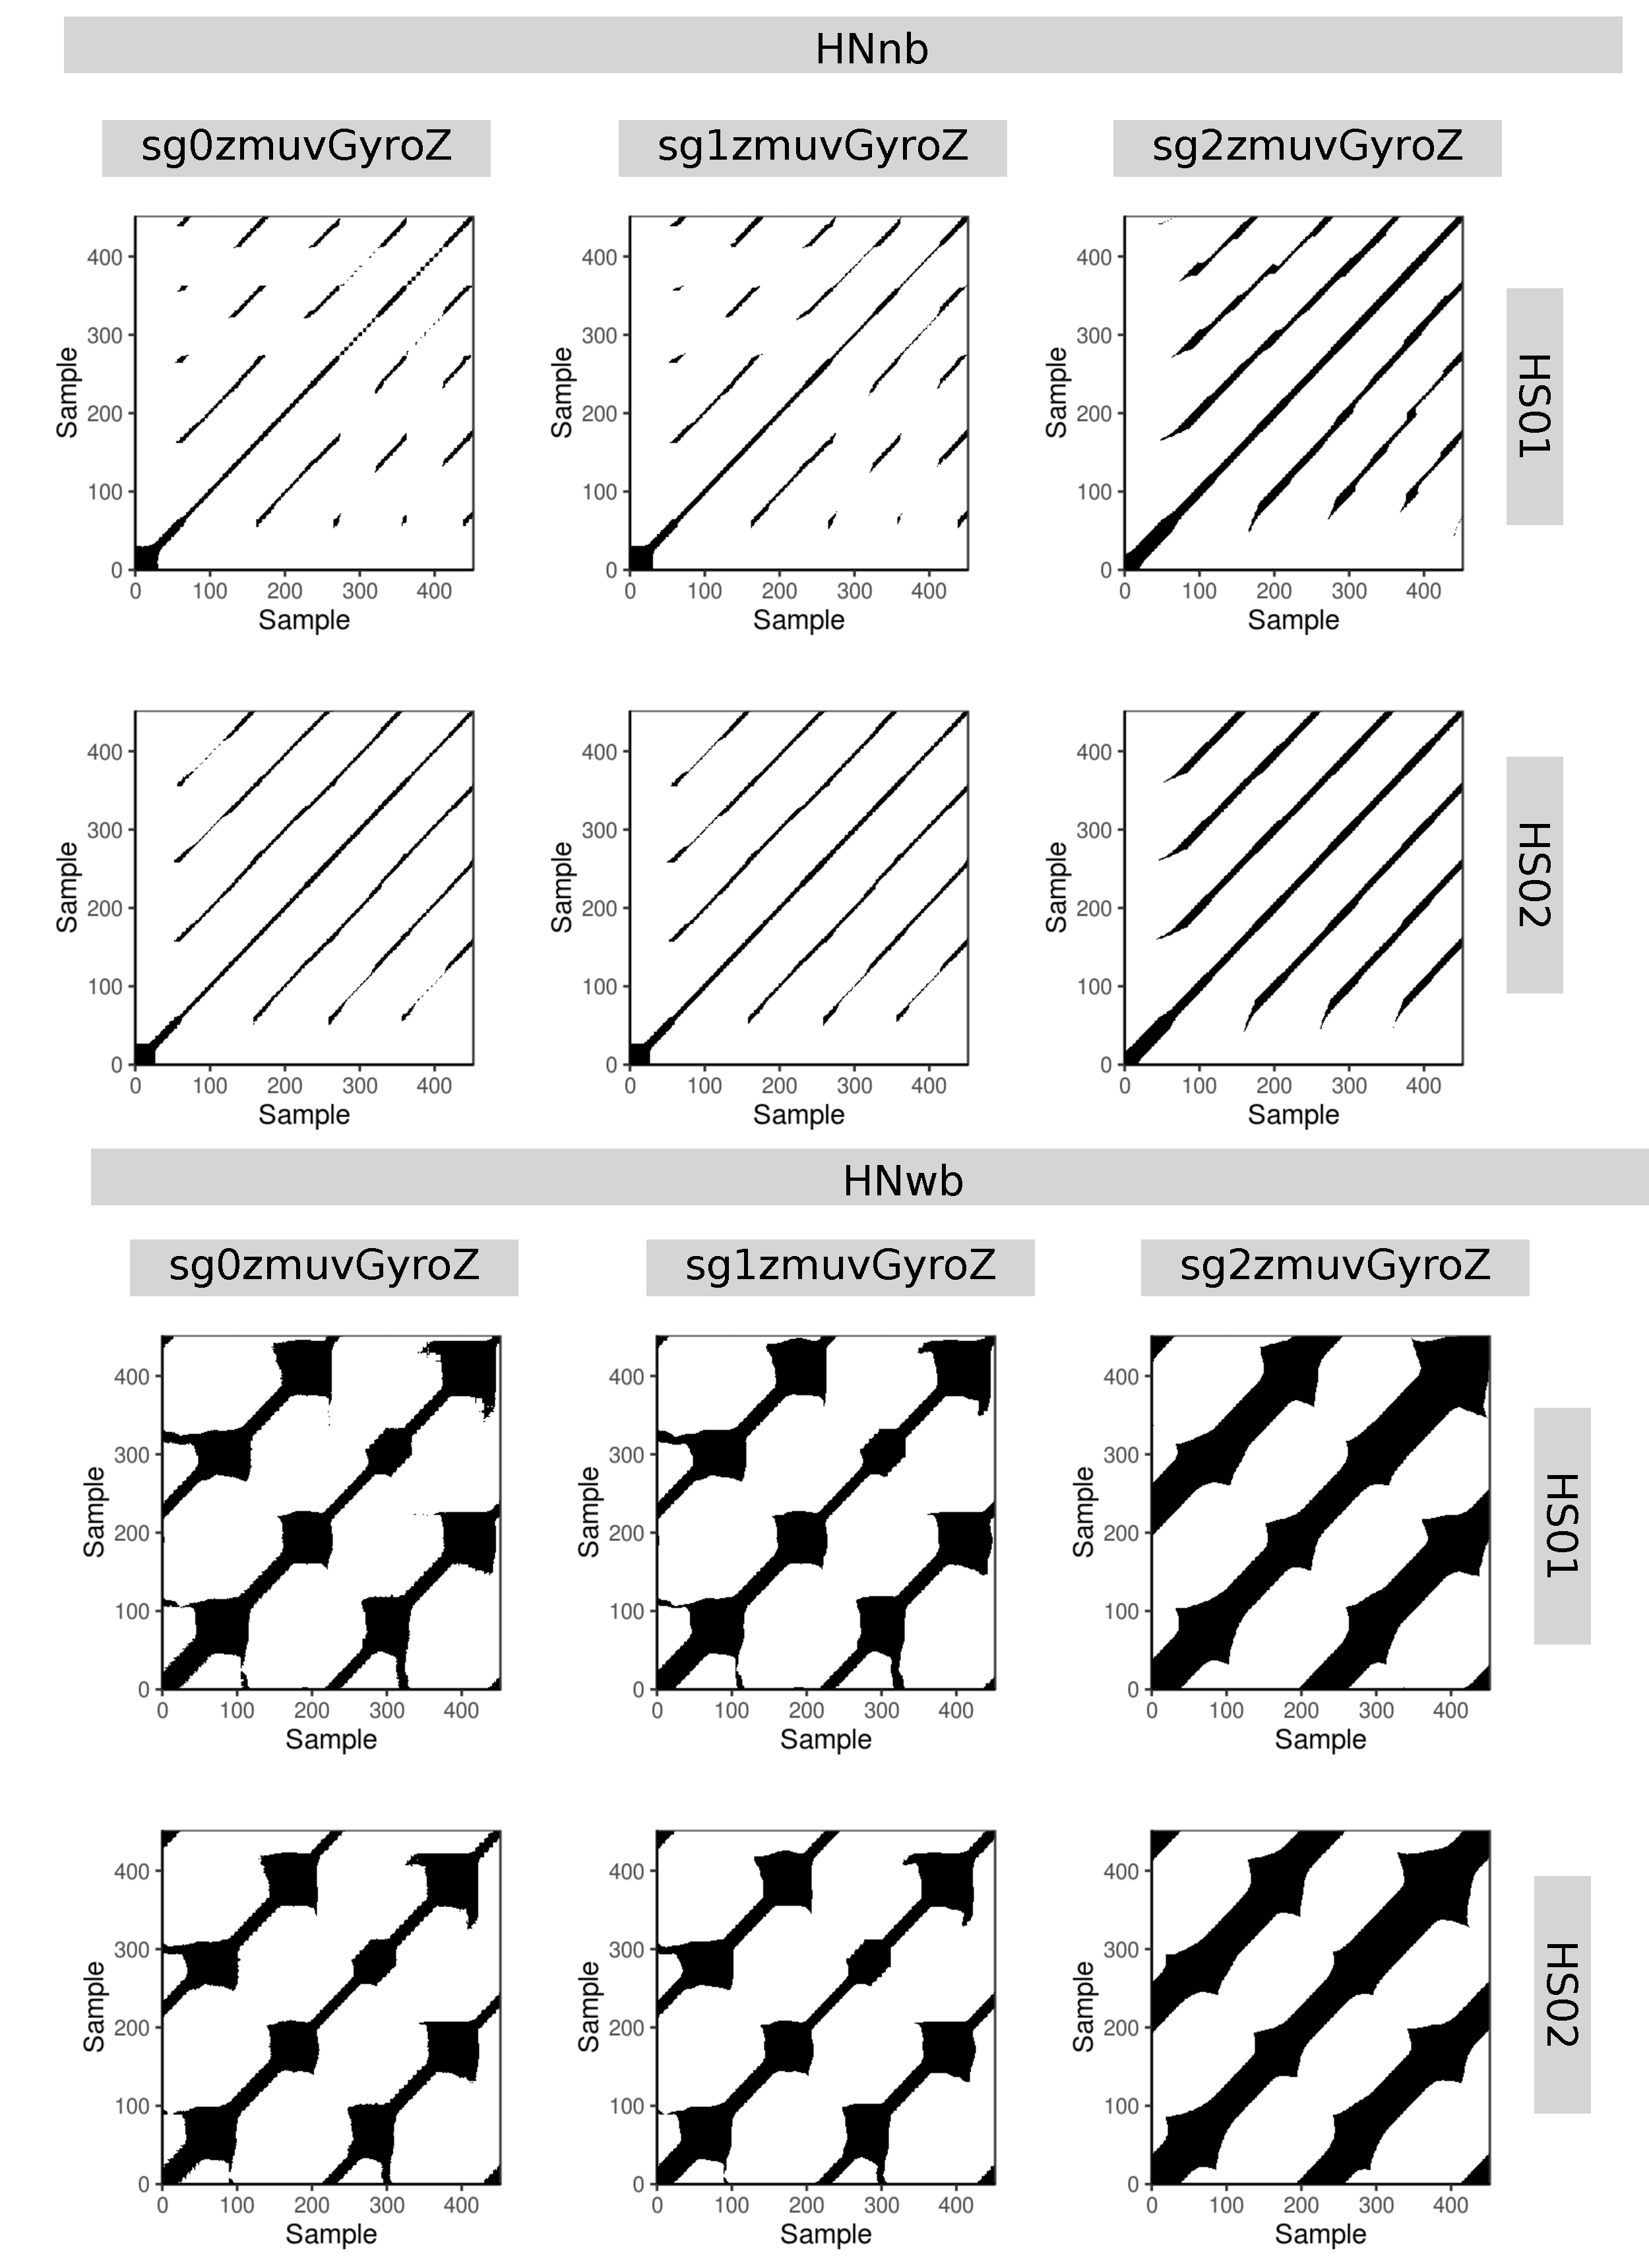
\includegraphics[height=0.8\textheight]{rps_HN_w500_p04}
\caption
	[RPs for horizontal normal arm movements]{
	{\bf RPs for horizontal normal arm movements.}	
	Recurrence plots of participant $p04$ for 
	horizontal normal movements with no beat (HNnb) and
	horizontal normal movements with beat (HFwb).
	Time series for raw-normalised (sg0zmuvGyroZ), 
	normalised-smoothed 1 (sg1zmuvGyroZ) and 
	normalised-smoothed 2 (sg2zmuvGyroZ) with
	sensors attached to the participant (HS01, HS02).
	Recurrence plots were computed with 
	embedding parameters $m=9$, $\tau=6$ and 
	recurrence threshold $\epsilon=1$.
	R code to reproduce the figure is available from \cite{hwum2018}.
        }
    \label{fig:rps_HN_w500_p04}
\end{figure}
%%---------------------------------(FIGURE)------------------------------------




%%---------------------------------(FIGURE)------------------------------------
\begin{figure}
\centering
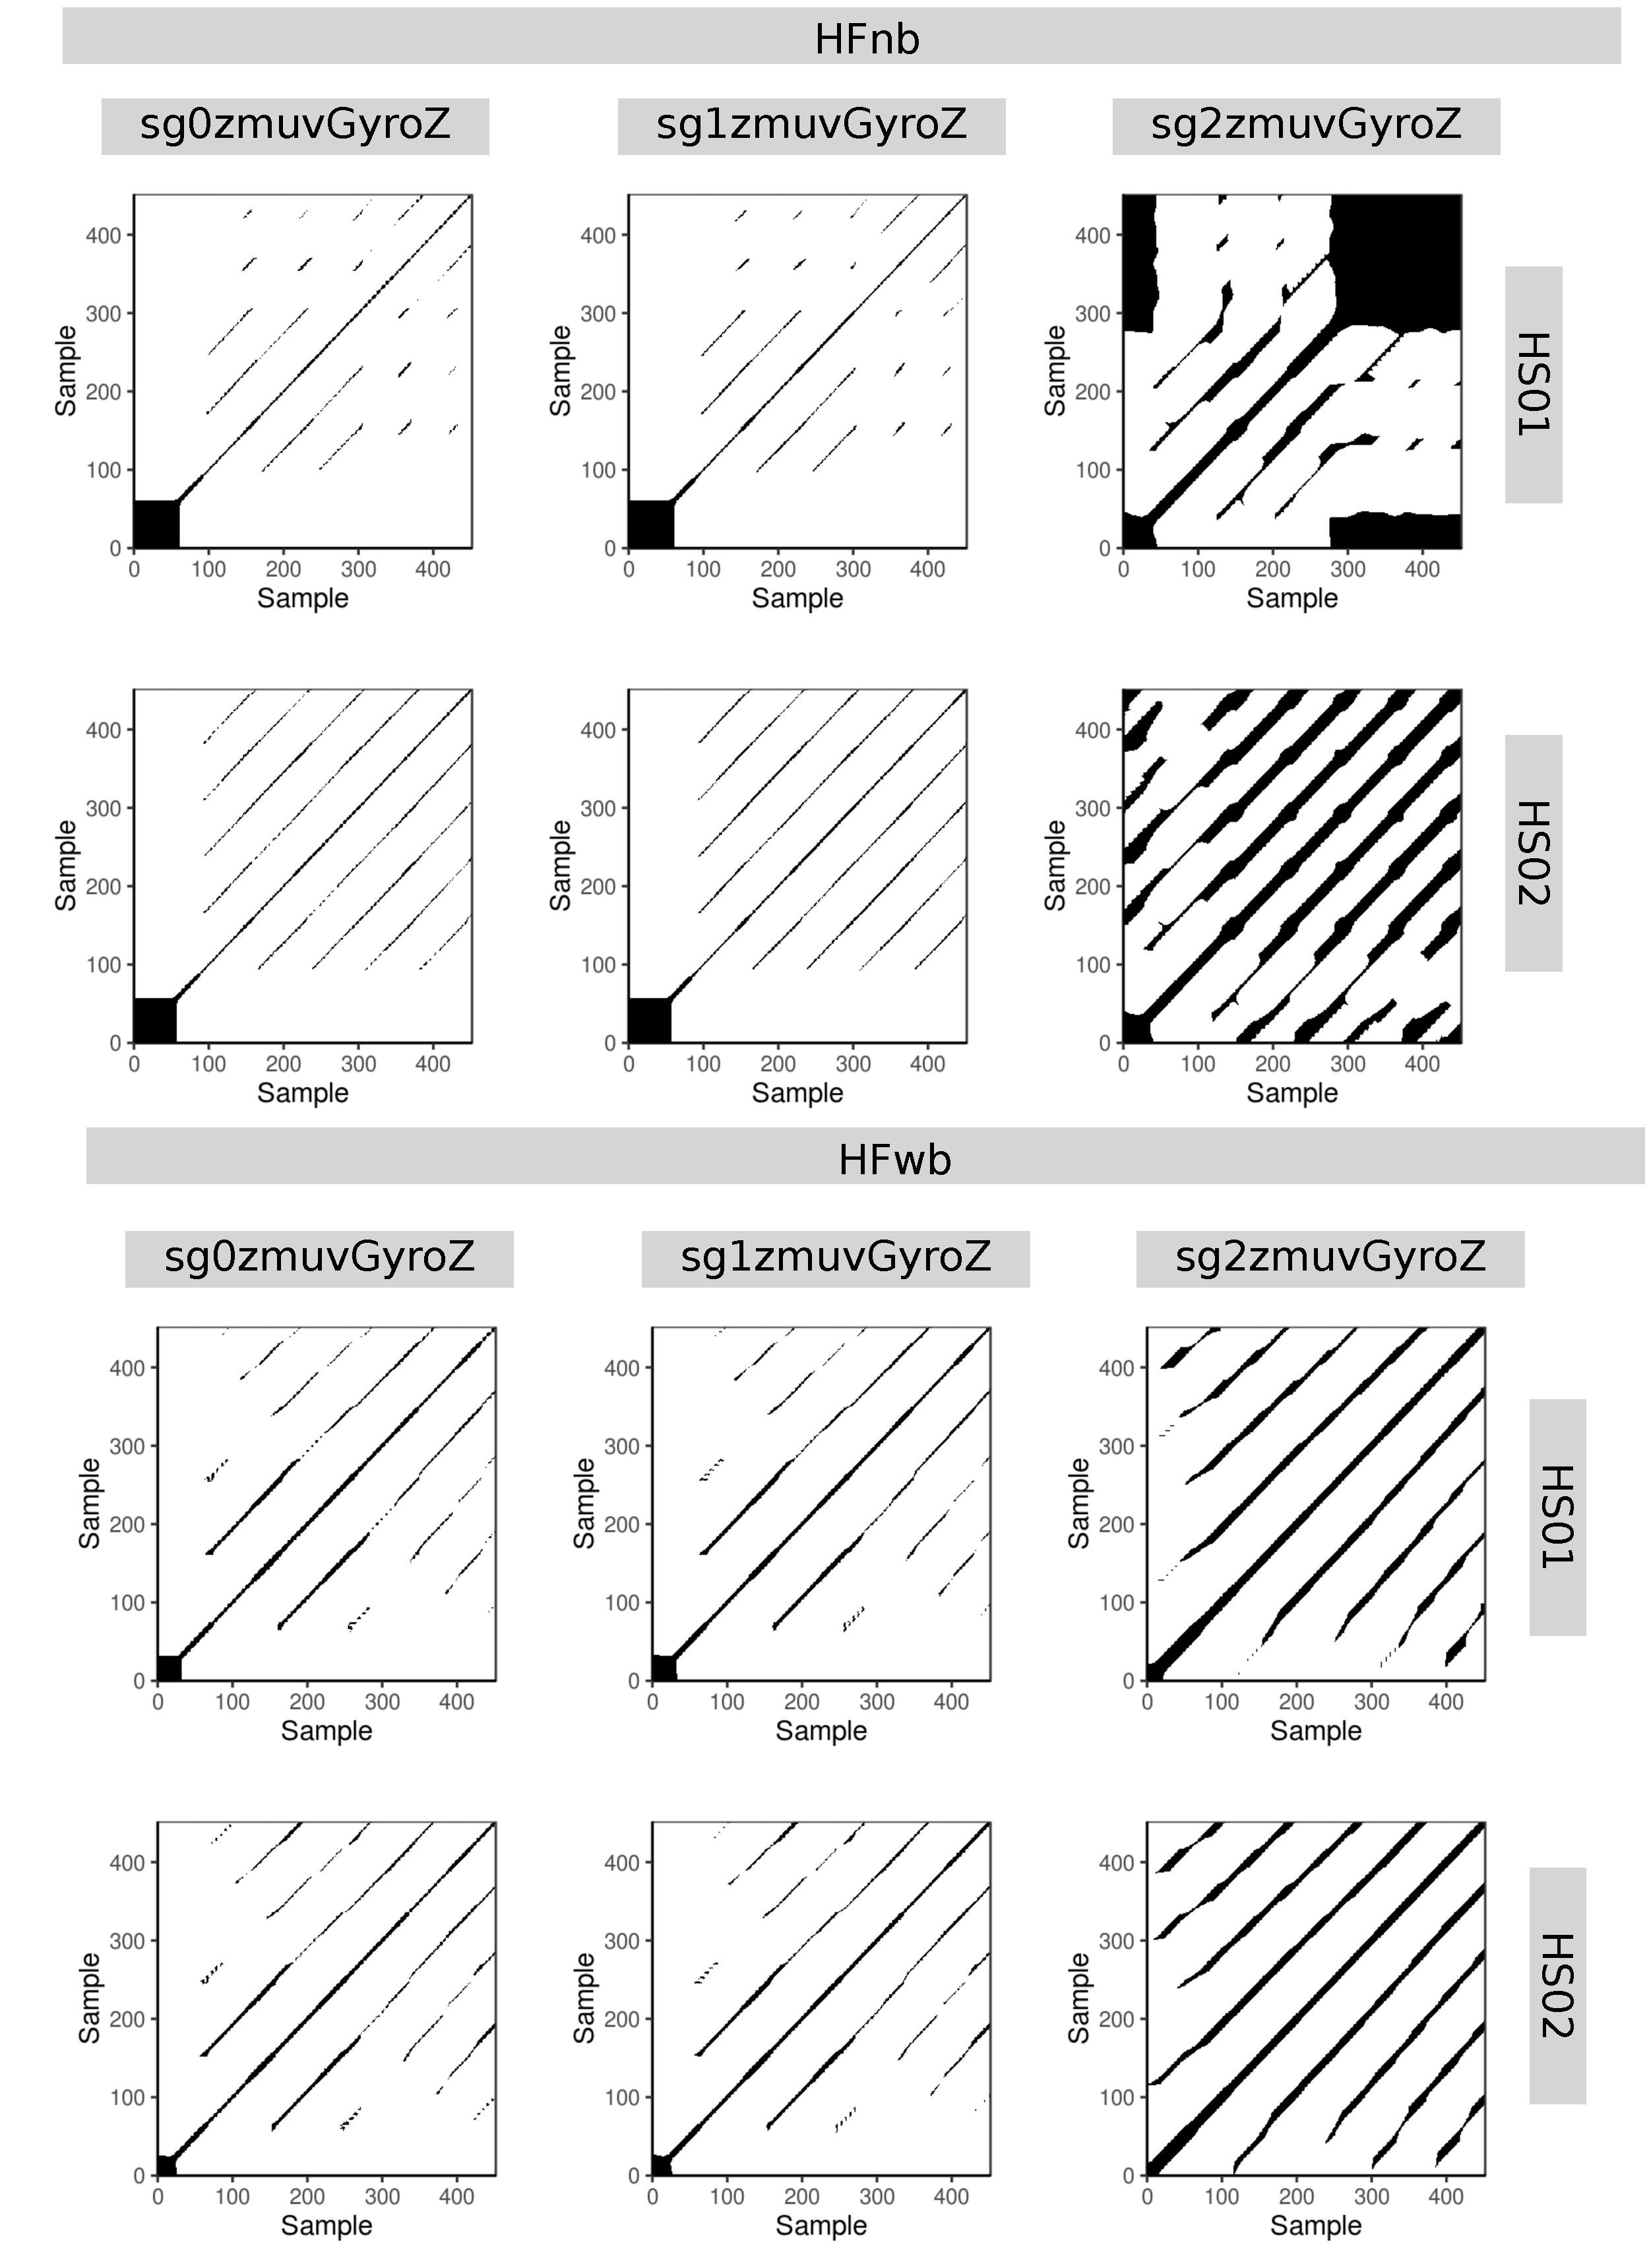
\includegraphics[height=0.8\textheight]{rps_HF_w500_p04}
\caption
	[RPs for horizontal faster arm movements]{
	{\bf RPs for horizontal faster arm movements.}	
	Recurrence plots of participant $p04$ for 
	horizontal faster movements with no beat (HNnb) and
	horizontal faster movements with beat (HFwb).
	Time series for raw-normalised (sg0zmuvGyroZ), 
	normalised-smoothed 1 (sg1zmuvGyroZ) and 
	normalised-smoothed 2 (sg2zmuvGyroZ) with
	sensors attached to the participant (HS01, HS02).
	Recurrence plots were computed with 
	embedding parameters $m=9$, $\tau=6$ and 
	recurrence threshold $\epsilon=1$.
	R code to reproduce the figure is available from \cite{hwum2018}.
        }
    \label{fig:rps_HF_w500_p04}
\end{figure}
%%---------------------------------(FIGURE)------------------------------------




%%---------------------------------(FIGURE)------------------------------------
\begin{figure}
\centering
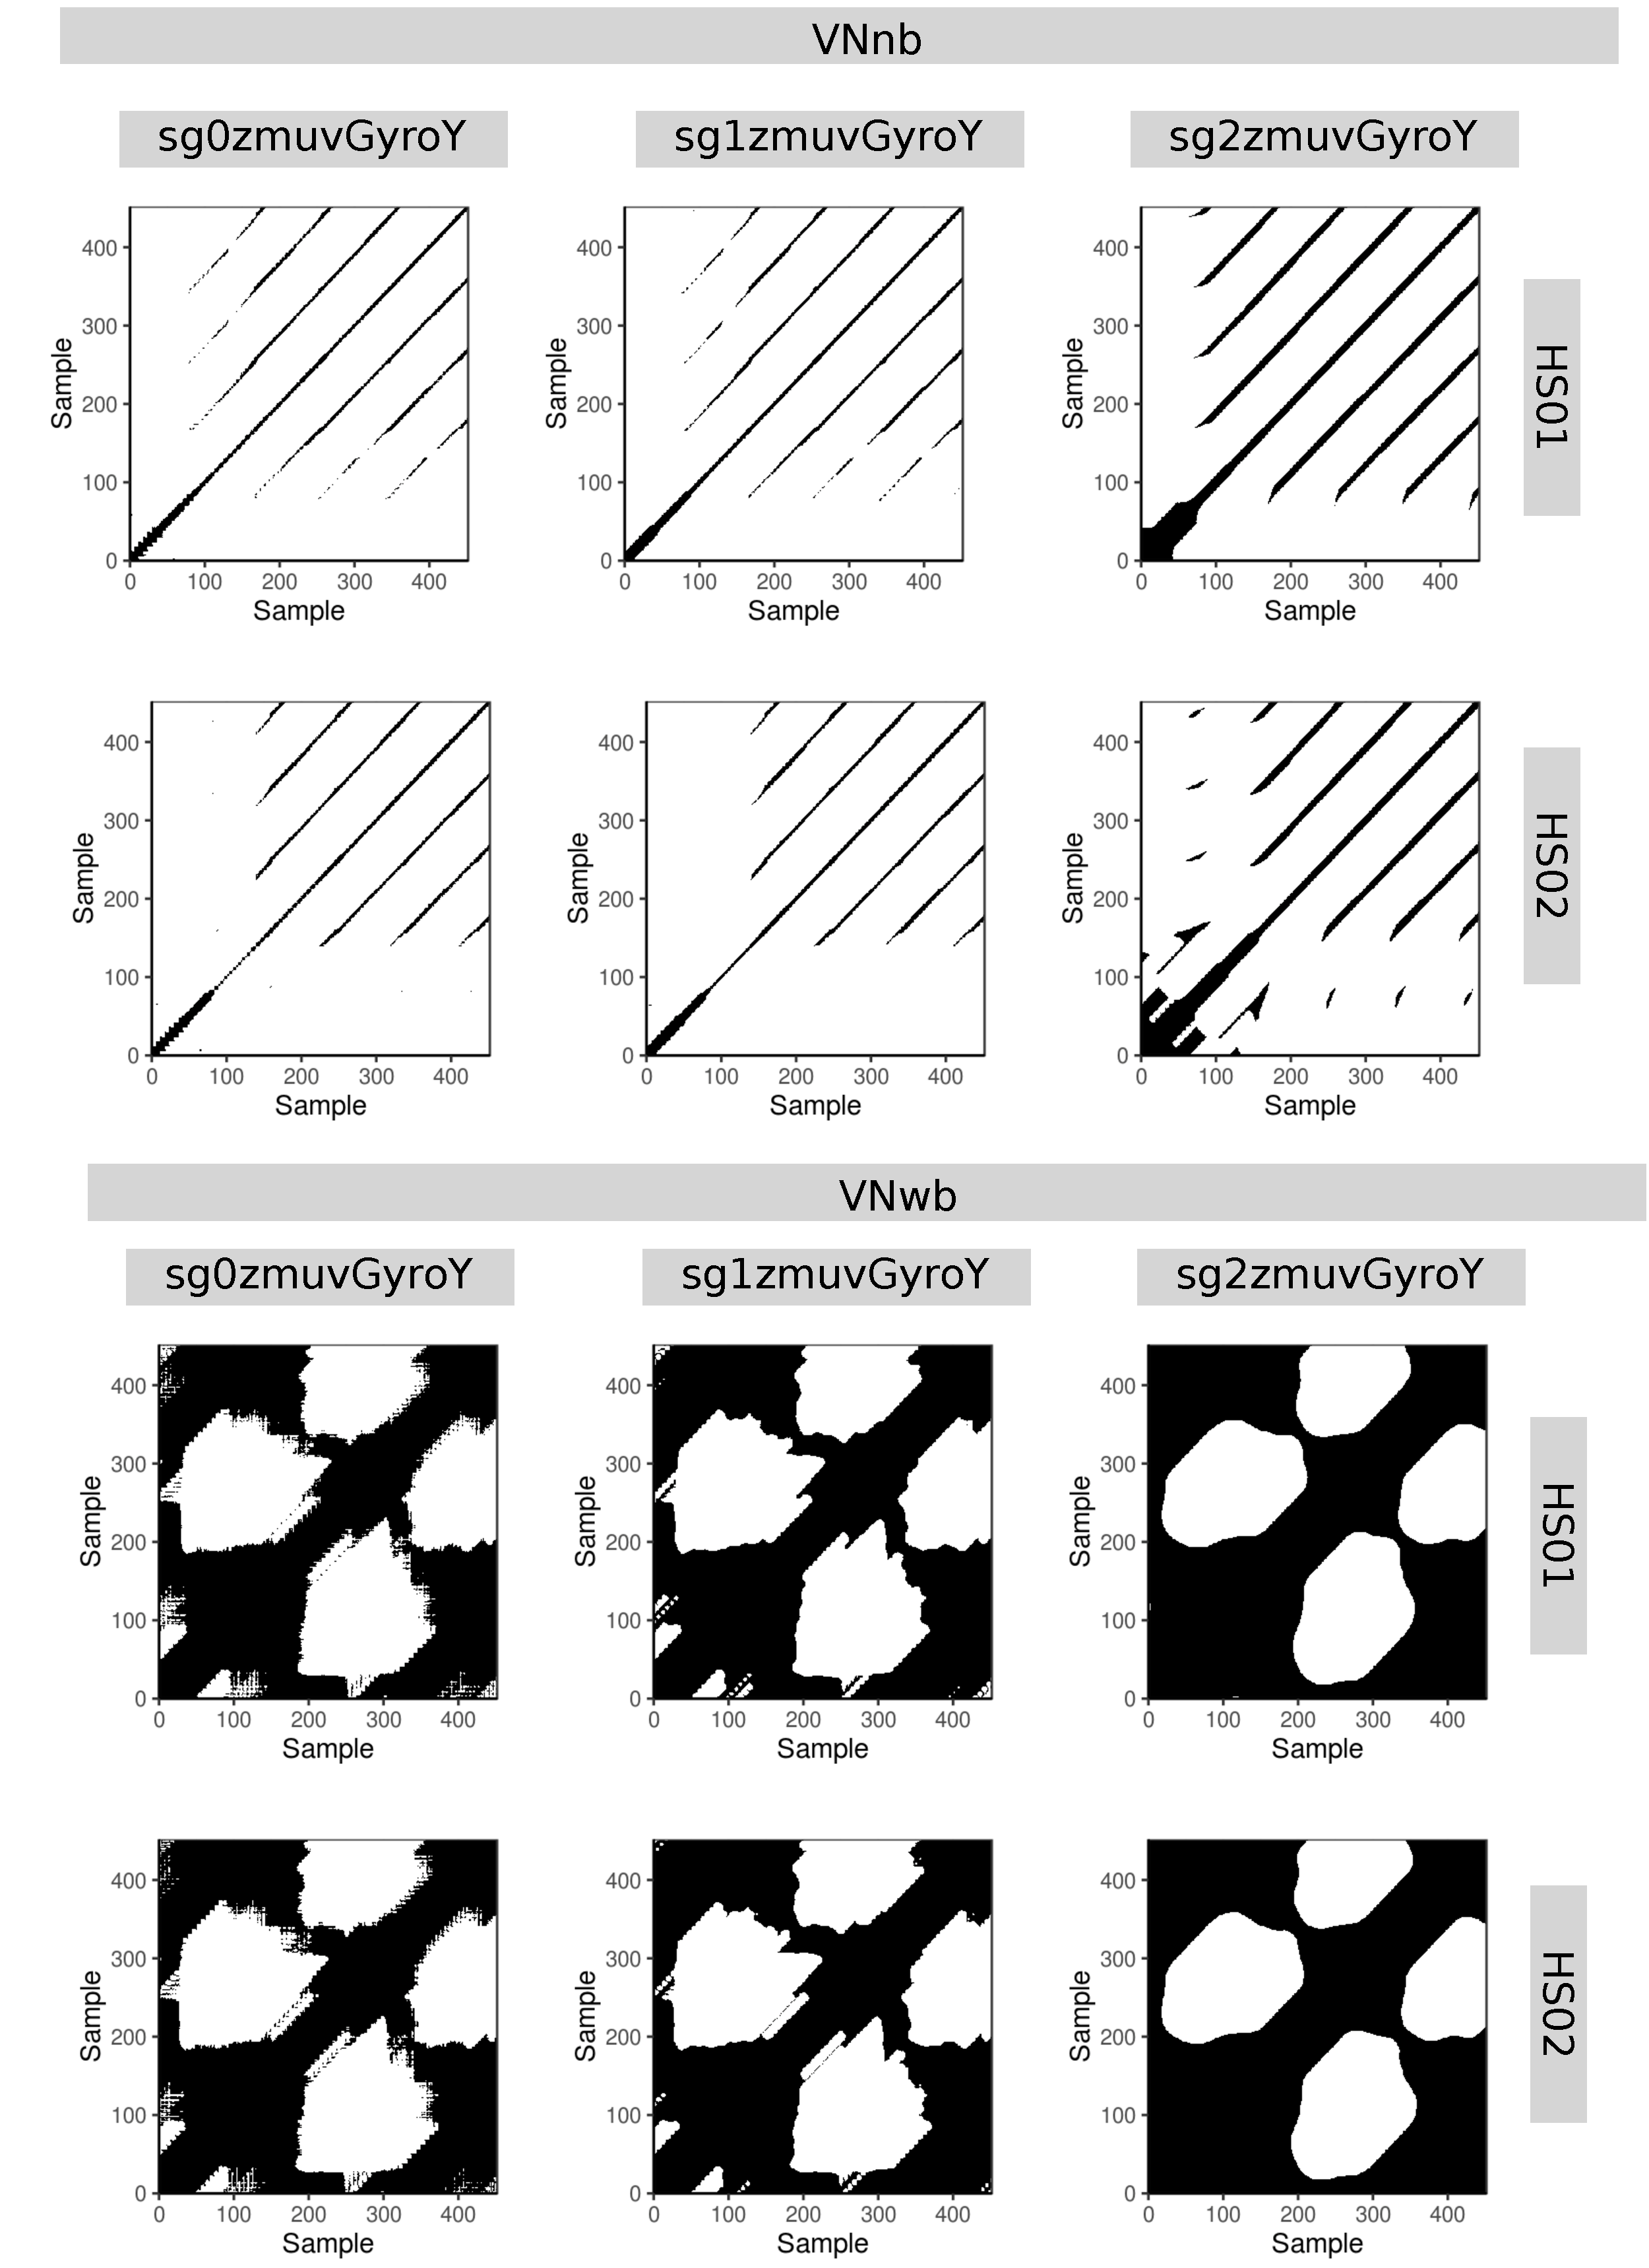
\includegraphics[height=0.8\textheight]{rps_VN_w500_p04}
\caption
	[RPs for vertical normal arm movements]{
	{\bf RPs for vertical normal arm movements.}	
	Recurrence plots of participant $p04$ for 
	horizontal normal movements with no beat (VNnb) and
	horizontal normal movements with beat (VFwb).
	Time series for raw-normalised (sg0zmuvGyroY), 
	normalised-smoothed 1 (sg1zmuvGyroY) and 
	normalised-smoothed 2 (sg2zmuvGyroY) with
	sensors attached to the participant (HS01, HS02).
	Recurrence plots were computed with 
	embedding parameters $m=9$, $\tau=6$ and 
	recurrence threshold $\epsilon=1$.
	R code to reproduce the figure is available from \cite{hwum2018}.
        }
    \label{fig:rps_VN_w500_p04}
\end{figure}
%%---------------------------------(FIGURE)------------------------------------




%%---------------------------------(FIGURE)------------------------------------
\begin{figure}
\centering
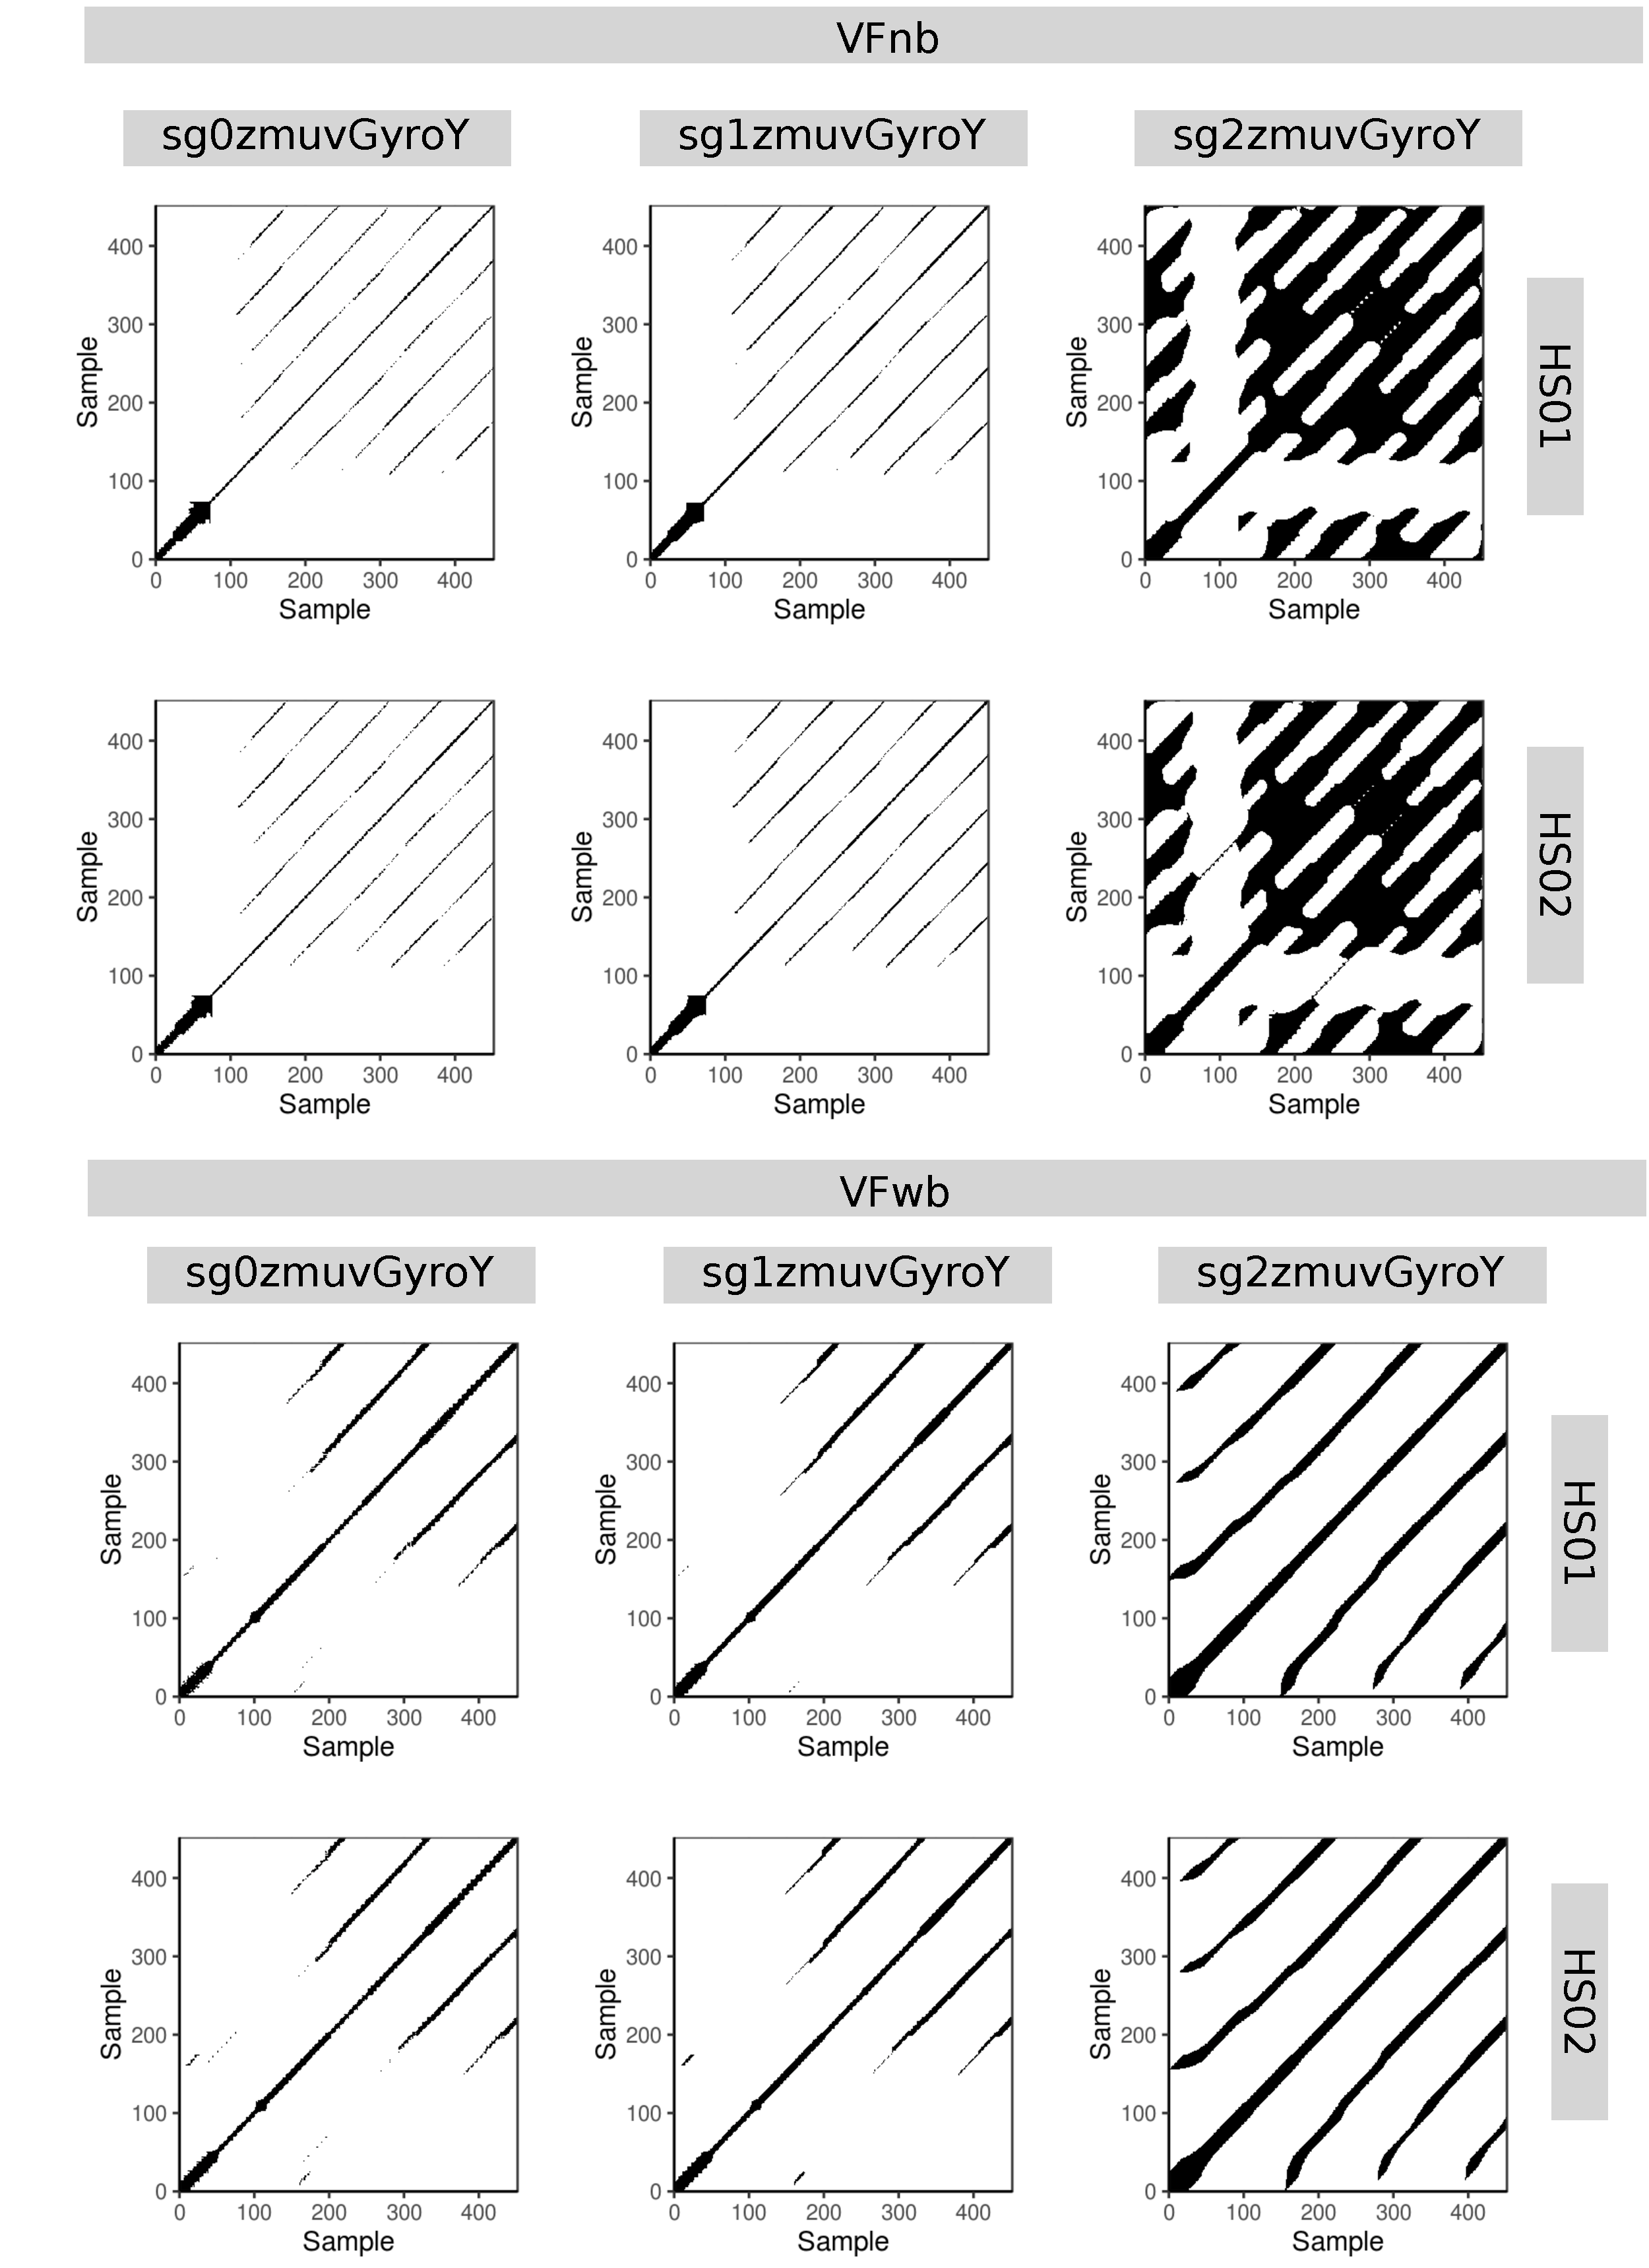
\includegraphics[height=0.8\textheight]{rps_VF_w500_p04}
\caption
	[RPs for vertical faster arm movements]{
	{\bf RPs for vertical faster arm movements.}	
	Recurrence plots of participant $p04$ for 
	horizontal faster movements with no beat (VNnb) and
	horizontal faster movements with beat (VFwb).
	Time series for raw-normalised (sg0zmuvGyroY), 
	normalised-smoothed 1 (sg1zmuvGyroY) and 
	normalised-smoothed 2 (sg2zmuvGyroY) with
	sensors attached to the participant (HS01, HS02).
	Recurrence plots were computed with 
	embedding parameters $m=9$, $\tau=6$ and 
	recurrence threshold $\epsilon=1$.
	R code to reproduce the figure is available from \cite{hwum2018}.
        }
    \label{fig:rps_VF_w500_p04}
\end{figure}
%%---------------------------------(FIGURE)------------------------------------







\newpage
\section{RQAs} \label{appendix:d:rpas}
\subsection{REC values}
Figs \ref{fig:rqa_rec_H} and \ref{fig:rqa_rec_V} show REC values,
representing the \% of black dots in the RPs, for vertical and horizontal 
arm movements.

It can be noted in Fig \ref{fig:rqa_rec_H} that REC values present 
little differences when comparing sensor HS01 and HS02. 
Similarly, considering the smoothness of the time series, REC values for 
participants appear to be similar in each of the activities 
(HNnb, HNwb, HFnb, HFwb) for sg0zmuvGyroZ and sg1zmuvGyroZ, 
while REC values for sg2zmuvGyroZ appear to fluctuate a bit more.
With regards to the type of activity, horizontal arm movements with beat 
(HNwb) appear to fluctuate more than other activities (HNnb, HFnb, HFwb). 
Also RET values appear to fluctuate more and be greater for faster
arm movements whereas RET values for normal arm movements appear 
to be constant (Fig \ref{fig:rqa_rec_H}).

Figs \ref{fig:rqa_rec_V} show RET values for vertical arm movements.
It can be noted that RET values appear to be similar for sensors HS01 and HS02
and the smoothness effect in REC values is more evident for sg2zmuvGyroY 
than REC values for sg0zmuvGyroY and sg1zmuvGyroY.
RET values appear to fluctuate more for vertical normal arm movements with 
beat (VNwb) than other activities (VNnb, VFnb, VFwb) and  RET values for 
VNnb, VFnb and VFwb appear to be constant and show little fluctuation 
between participants.




%%---------------------------------(FIGURE)------------------------------------
\begin{figure}
\centering
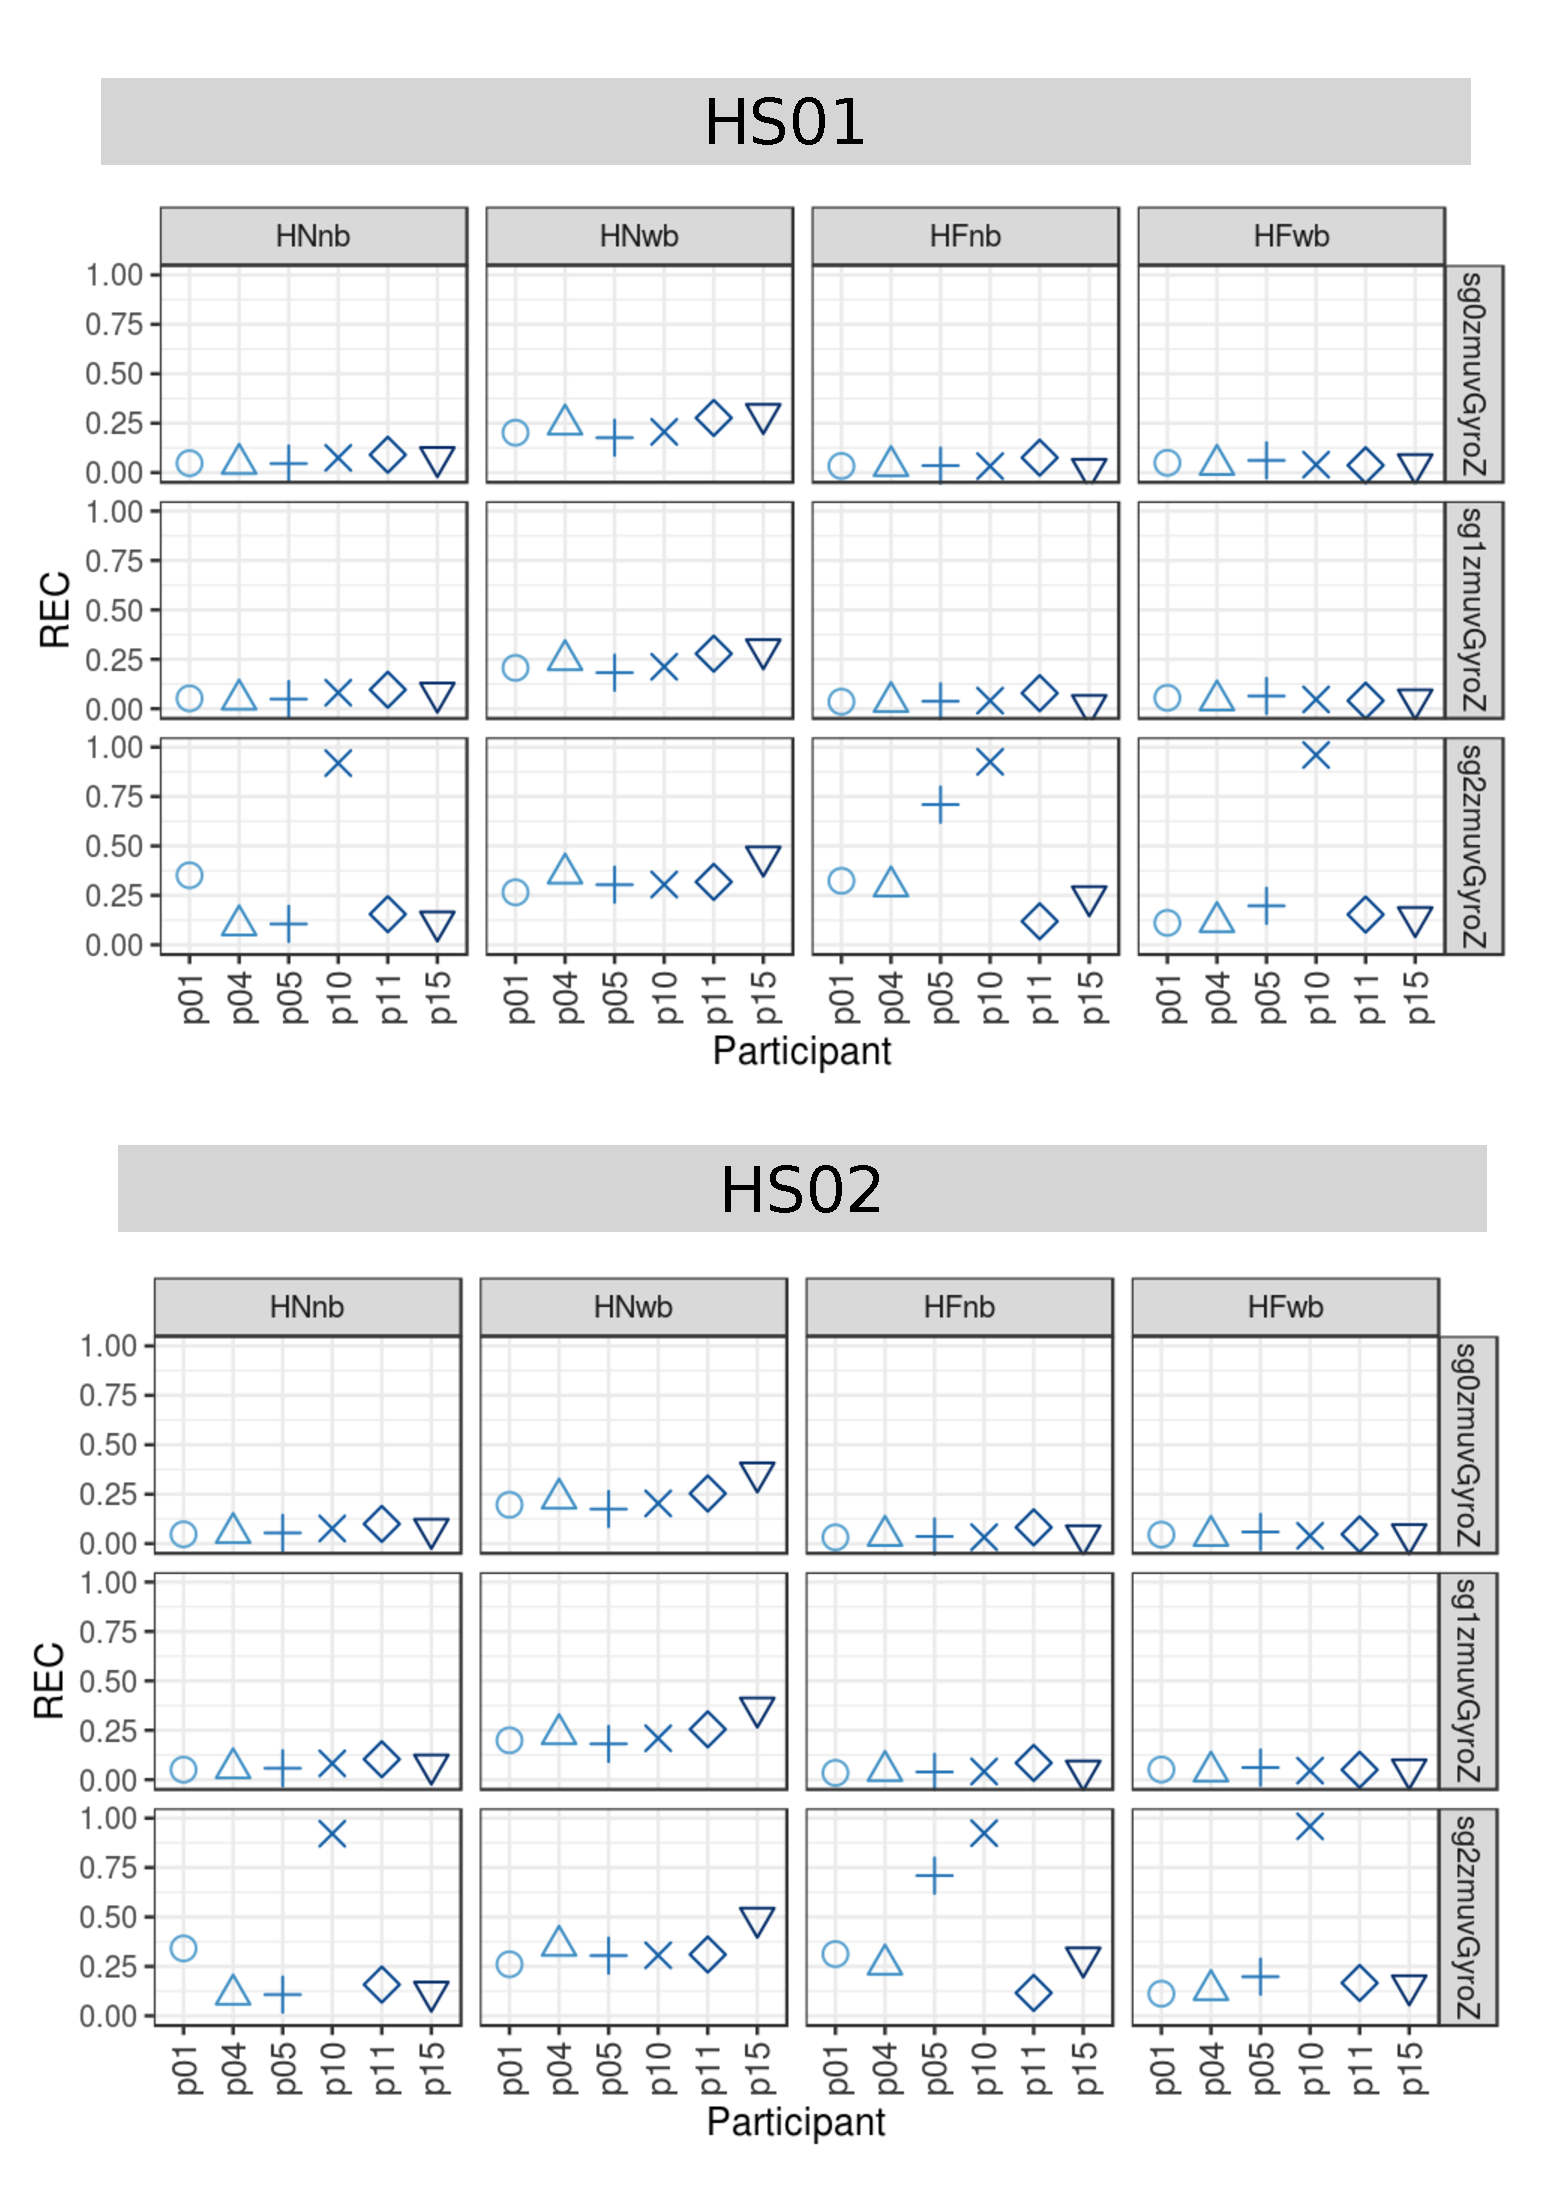
\includegraphics[width=0.9\textwidth]{rqa_rec_H_w500}
    \caption
	[REC values for horizontal arm movements]{
	{\bf REC values for horizontal arm movements.}	
	REC values (representing \% of black dots in the RPs) for 
	6 participants performing horizontal arm movements 
	(HNnb, HNwb, HFnb, HFwb)
	for sensors HS01, HS02 and three smoothed-normalised axis 
	of GyroZ (sg0zmuvGyroZ, sg1zmuvGyroZ and sg2zmuvGyroZ).
	REC values were computed with 
	embedding parameters $m=9$, $\tau=6$ and recurrence threshold
	$\epsilon=1$.
	R code to reproduce the figure is available from \cite{hwum2018}.
        }
    \label{fig:rqa_rec_H}
\end{figure}
%%---------------------------------(FIGURE)------------------------------------
%%---------------------------------(FIGURE)------------------------------------
\begin{figure}
\centering
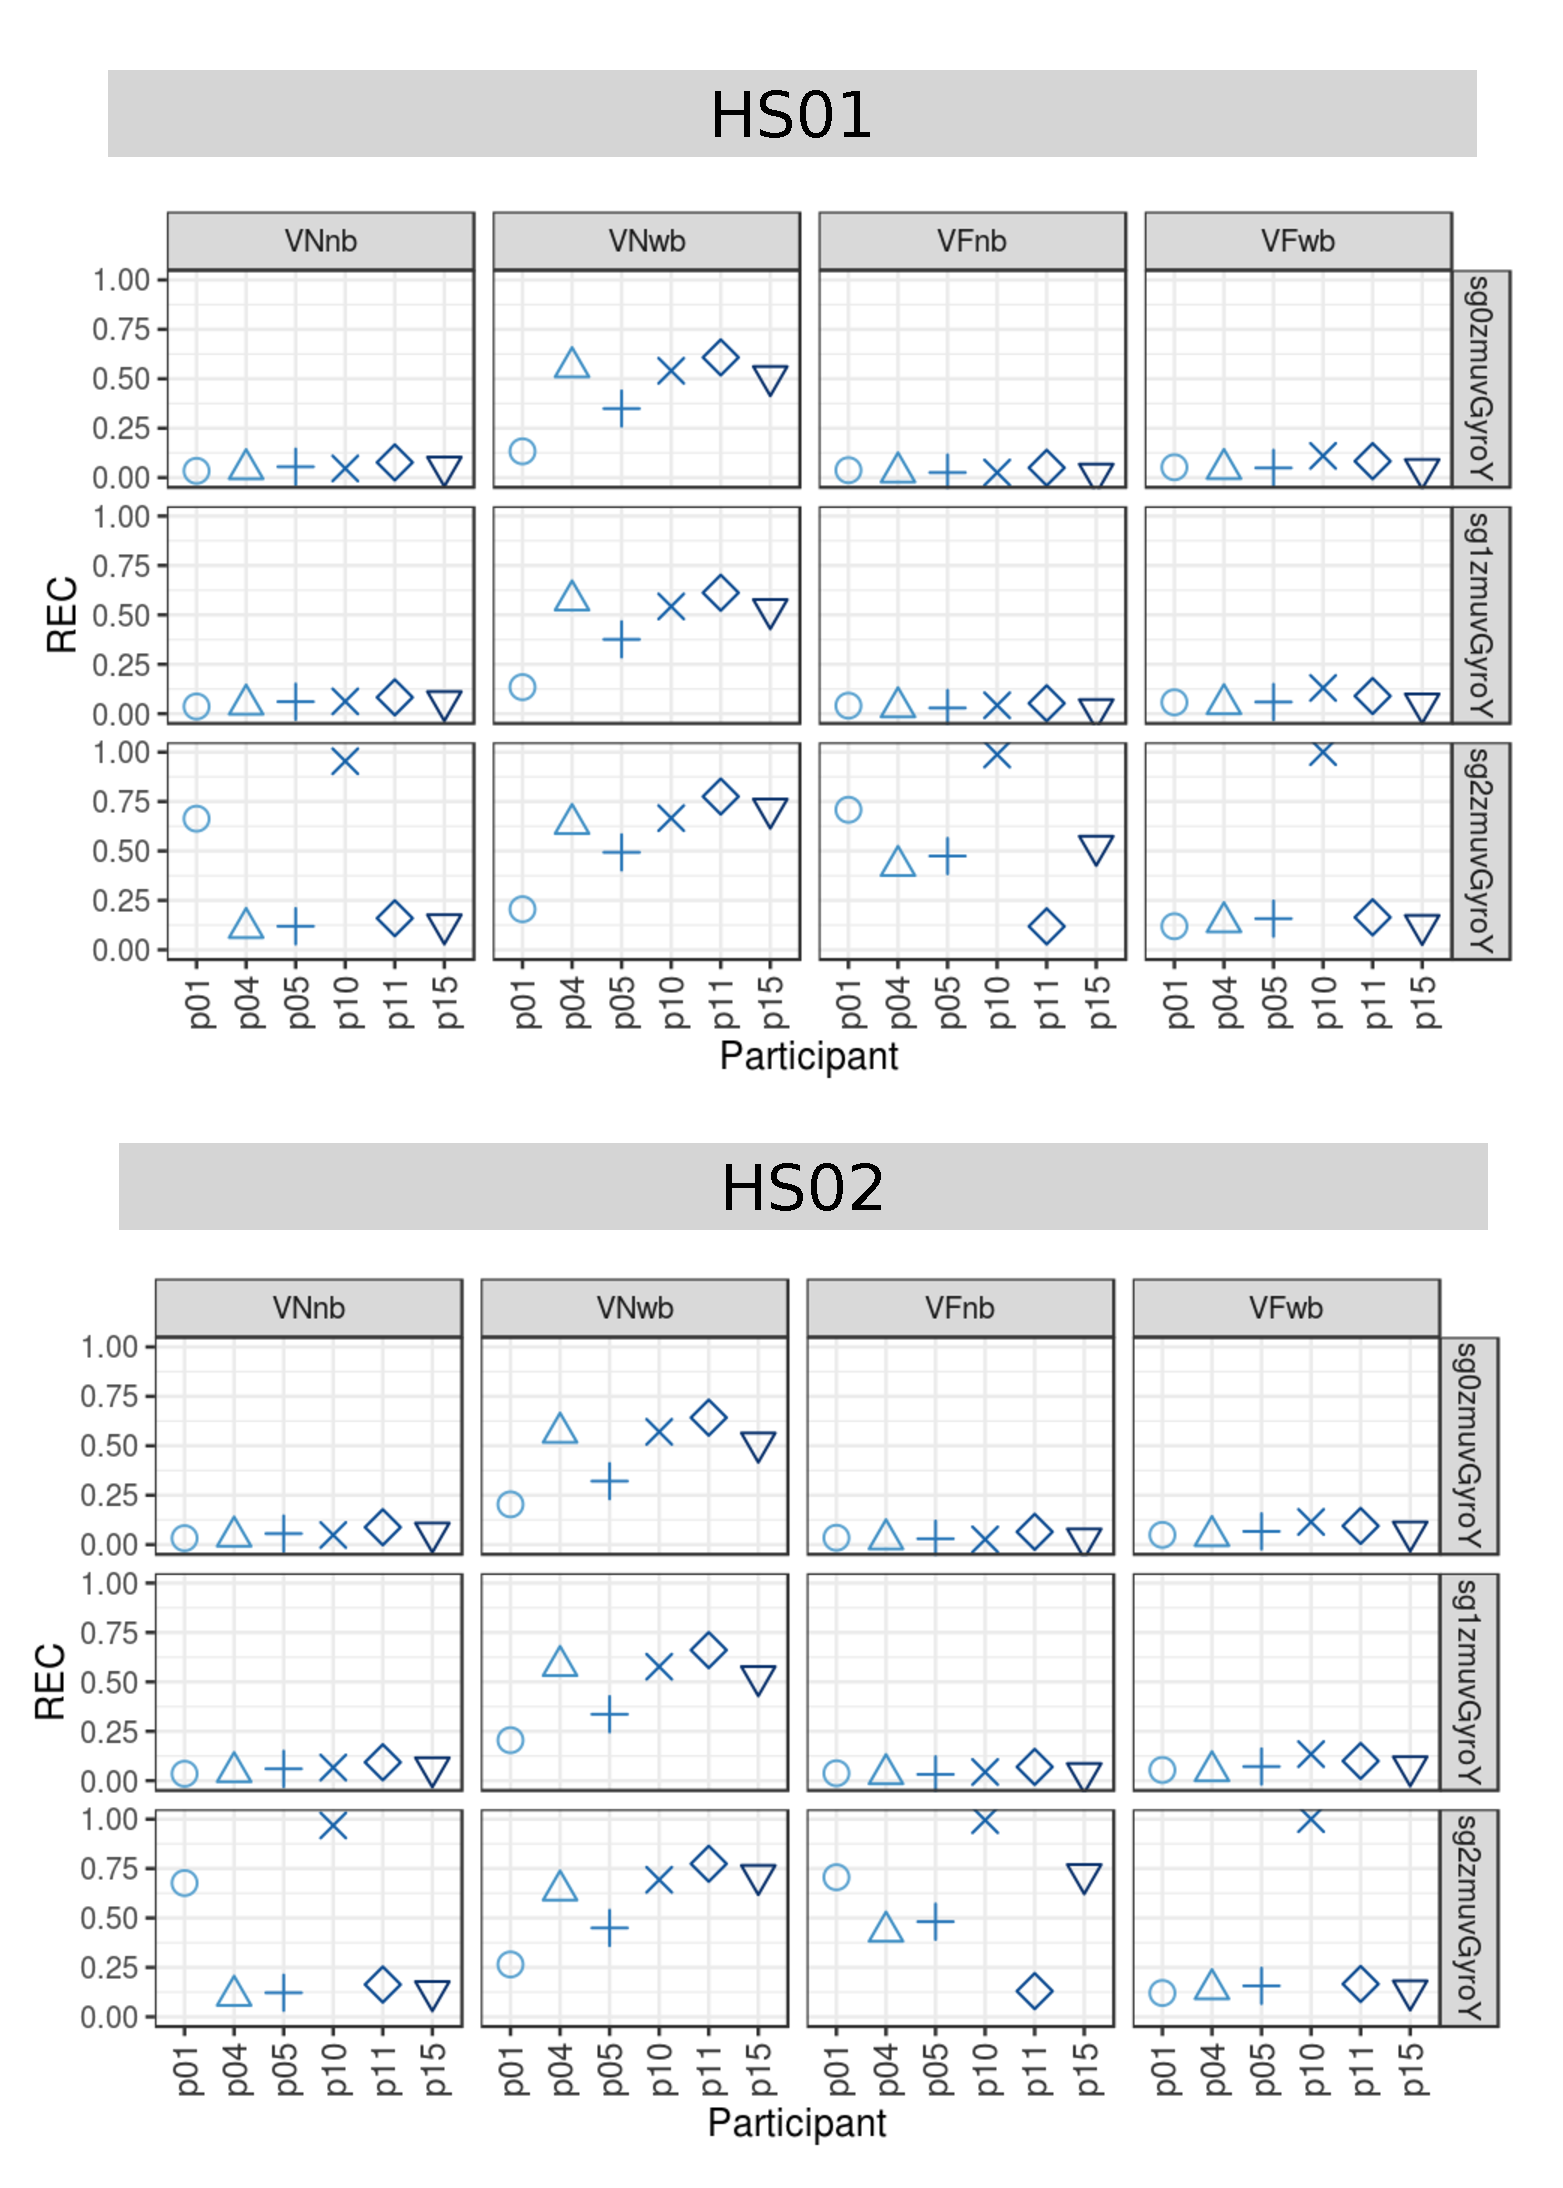
\includegraphics[width=0.9\textwidth]{rqa_rec_V_w500}
    \caption
	[REC values for vertical arm movements]{
	{\bf REC values for vertical arm movements.}
	REC values (representing \% of black dots in the RPs) for 
	6 participants performing vertical arm movements 
	(VNnb, VNwb, VFnb, VFwb)
	for sensors HS01, HS02 and three smoothed-normalised axis 
	of GyroZ (sg0zmuvGyroZ, sg1zmuvGyroZ and sg2zmuvGyroZ).
	REC values were computed with 
	embedding parameters $m=9$, $\tau=6$ and recurrence threshold
	$\epsilon=1$.
	R code to reproduce the figure is available from \cite{hwum2018}.
        }
    \label{fig:rqa_rec_V}
\end{figure}
%%---------------------------------(FIGURE)------------------------------------


\newpage
\subsection{DET values}

DET values appear to be constant for any source of time series 
(Figs \ref{fig:rqa_det_H} and \ref{fig:rqa_det_V}).
For both horizontal and vertical arm movements, the increase of smoothness 
of time series appear to affect the smoothness of DET values by making them 
to appear more similar as the smoothness increase.
Additionally, it can be noted more fluctuations of DET values 
for faster activities (HFnb, HFwb) 
than normal activities (HNnb, HNwb), specifically for  sg0zmuvGyroY 
(Figs \ref{fig:rqa_det_H}, \ref{fig:rqa_det_V}).




%%---------------------------------(FIGURE)------------------------------------
\begin{figure}
\centering
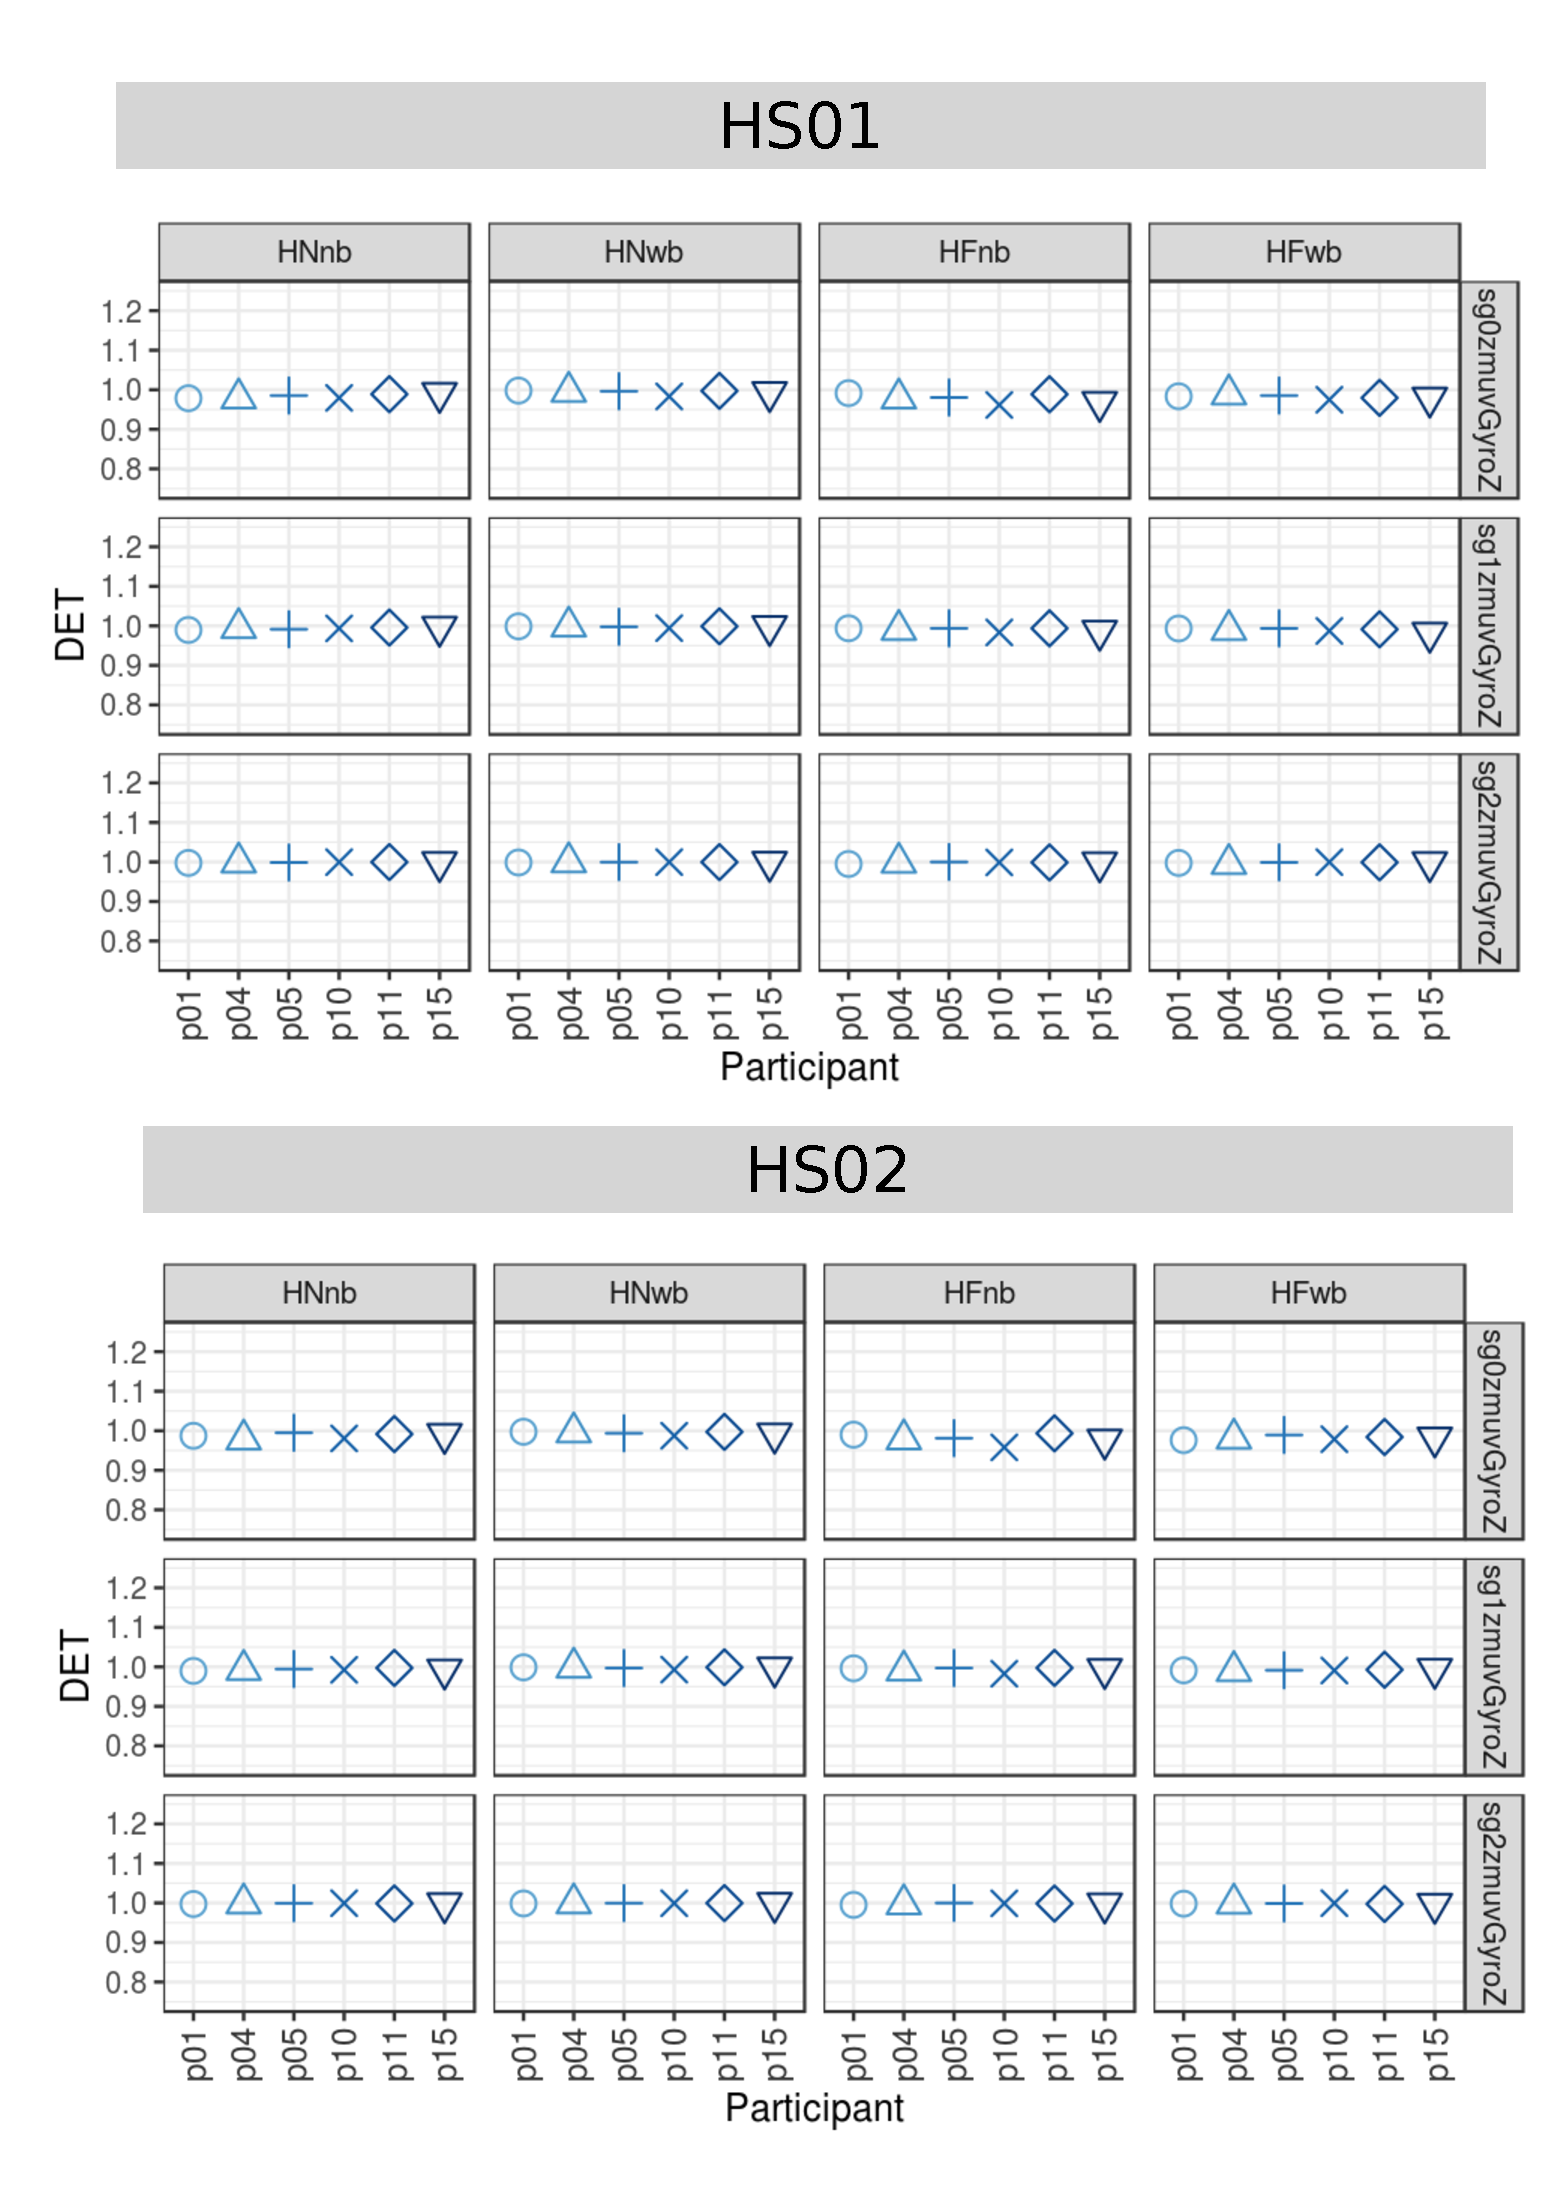
\includegraphics[width=0.9\textwidth]{rqa_det_H_w500}
    \caption
	[DET values for horizontal arm movements]{
	{\bf DET values for horizontal arm movements.}	
    	DET values (representing predictability and organisation of the RPs)
	for 6 participants performing horizontal arm movements 
	(HNnb, HNwb, HFnb, HFwb)
	for sensors HS01, HS02 and three smoothed-normalised axis 
	of GyroZ (sg0zmuvGyroZ, sg1zmuvGyroZ and sg2zmuvGyroZ).
	DET values were computed with 
	embedding parameters $m=9$, $\tau=6$ and recurrence threshold
	$\epsilon=1$.
	R code to reproduce the figure is available from \cite{hwum2018}.
        }
    \label{fig:rqa_det_H}
\end{figure}
%%---------------------------------(FIGURE)------------------------------------
%%---------------------------------(FIGURE)------------------------------------
\begin{figure}
\centering
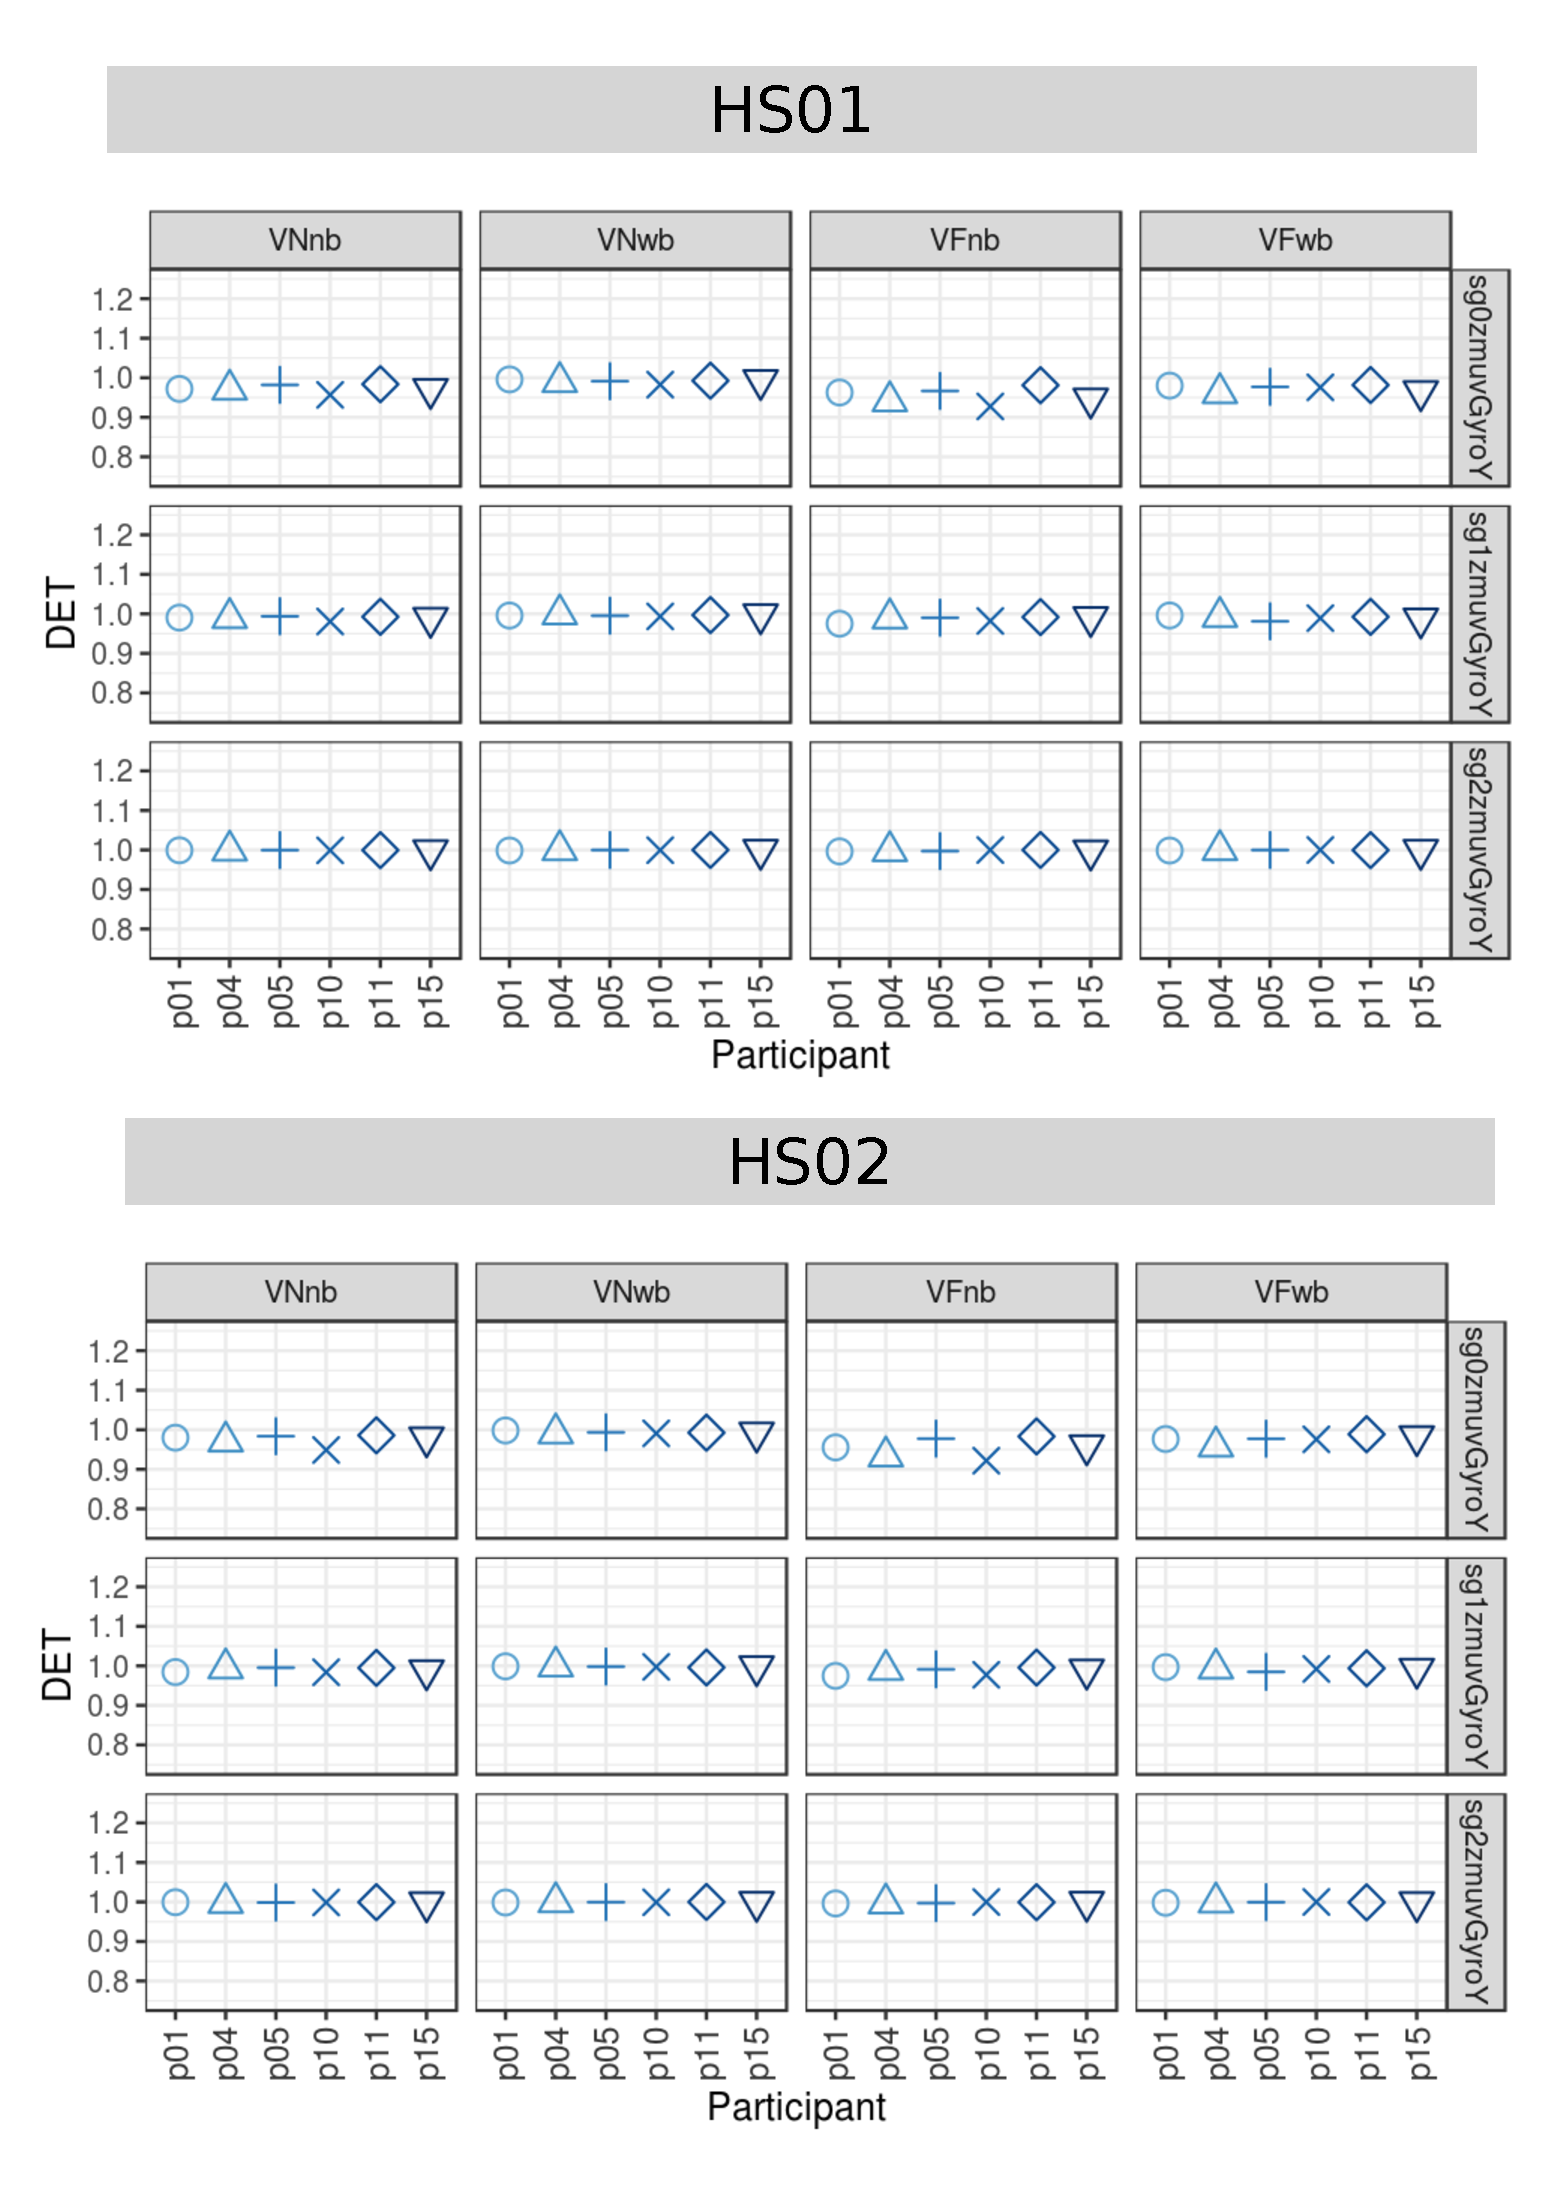
\includegraphics[width=0.9\textwidth]{rqa_det_V_w500}
    \caption
	[DET values for vertical arm movements]{
	{\bf DET values for vertical arm movements.}	
    	DET values (representing predictability and organisation of the RPs)
	for 6 participants performing vertical arm movements 
	(VNnb, VNwb, VFnb, VFwb)
	for sensors HS01, HS02 and three smoothed-normalised axis 
	of GyroY (sg0zmuvGyroY, sg1zmuvGyroY and sg2zmuvGyroY).
	DET values were computed with 
	embedding parameters $m=9$, $\tau=6$ and recurrence threshold
	$\epsilon=1$.
	R code to reproduce the figure is available from \cite{hwum2018}.
        }
    \label{fig:rqa_det_V}
\end{figure}
%%---------------------------------(FIGURE)------------------------------------


\newpage
\subsection{RATIO values}

RATIO values for horizontal and 
vertical arm movements are shown in Figs \ref{fig:rqa_ratio_H} and 
\ref{fig:rqa_ratio_V}.

The fluctuation of RATIO values for horizontal faster arm movements 
appear to be more notable than RATIO values for horizontal normal arm 
movements. RATIO values appear to be constant for activity HNwb than
other activities (HNnb, HFnb, HFwb).
Regarding the smoothness of time series, RATIO values appear to have 
similar values for sg0zmuvGyroZ and sg1zmuvGyroZ while RATIOS values 
are more uniform for sg2zmuvGyroZ.
With regards to type of sensor, 
RET values appear to be similar for HS01 and HS02 with the exception of
$p15$ in HFnb activity (Figs \ref{fig:rqa_ratio_H}).

Figs \ref{fig:rqa_ratio_V} show RATIO values for vertical arm movements.
The fluctuation of RATIO values appears to be constant for the activity 
VNwb whereas other RATIO values for other activities (VNnb, VFnb, VFwb) 
appear to fluctuate more.
The smoothness of the time series affects only the RATIO values for 
sg2zmuvGyroY as these appear to be constant, while RET values for 
sg0zmuvGyroY and sg1zmuvGyroZ appear to have the similar RATIO values.
Additionally, RATIO values for type of sensors HS01 and HS02 appear 
to show similar values as well, with the exception of $p15$ in the 
VFnb activity.




%%---------------------------------(FIGURE)------------------------------------
\begin{figure}
\centering
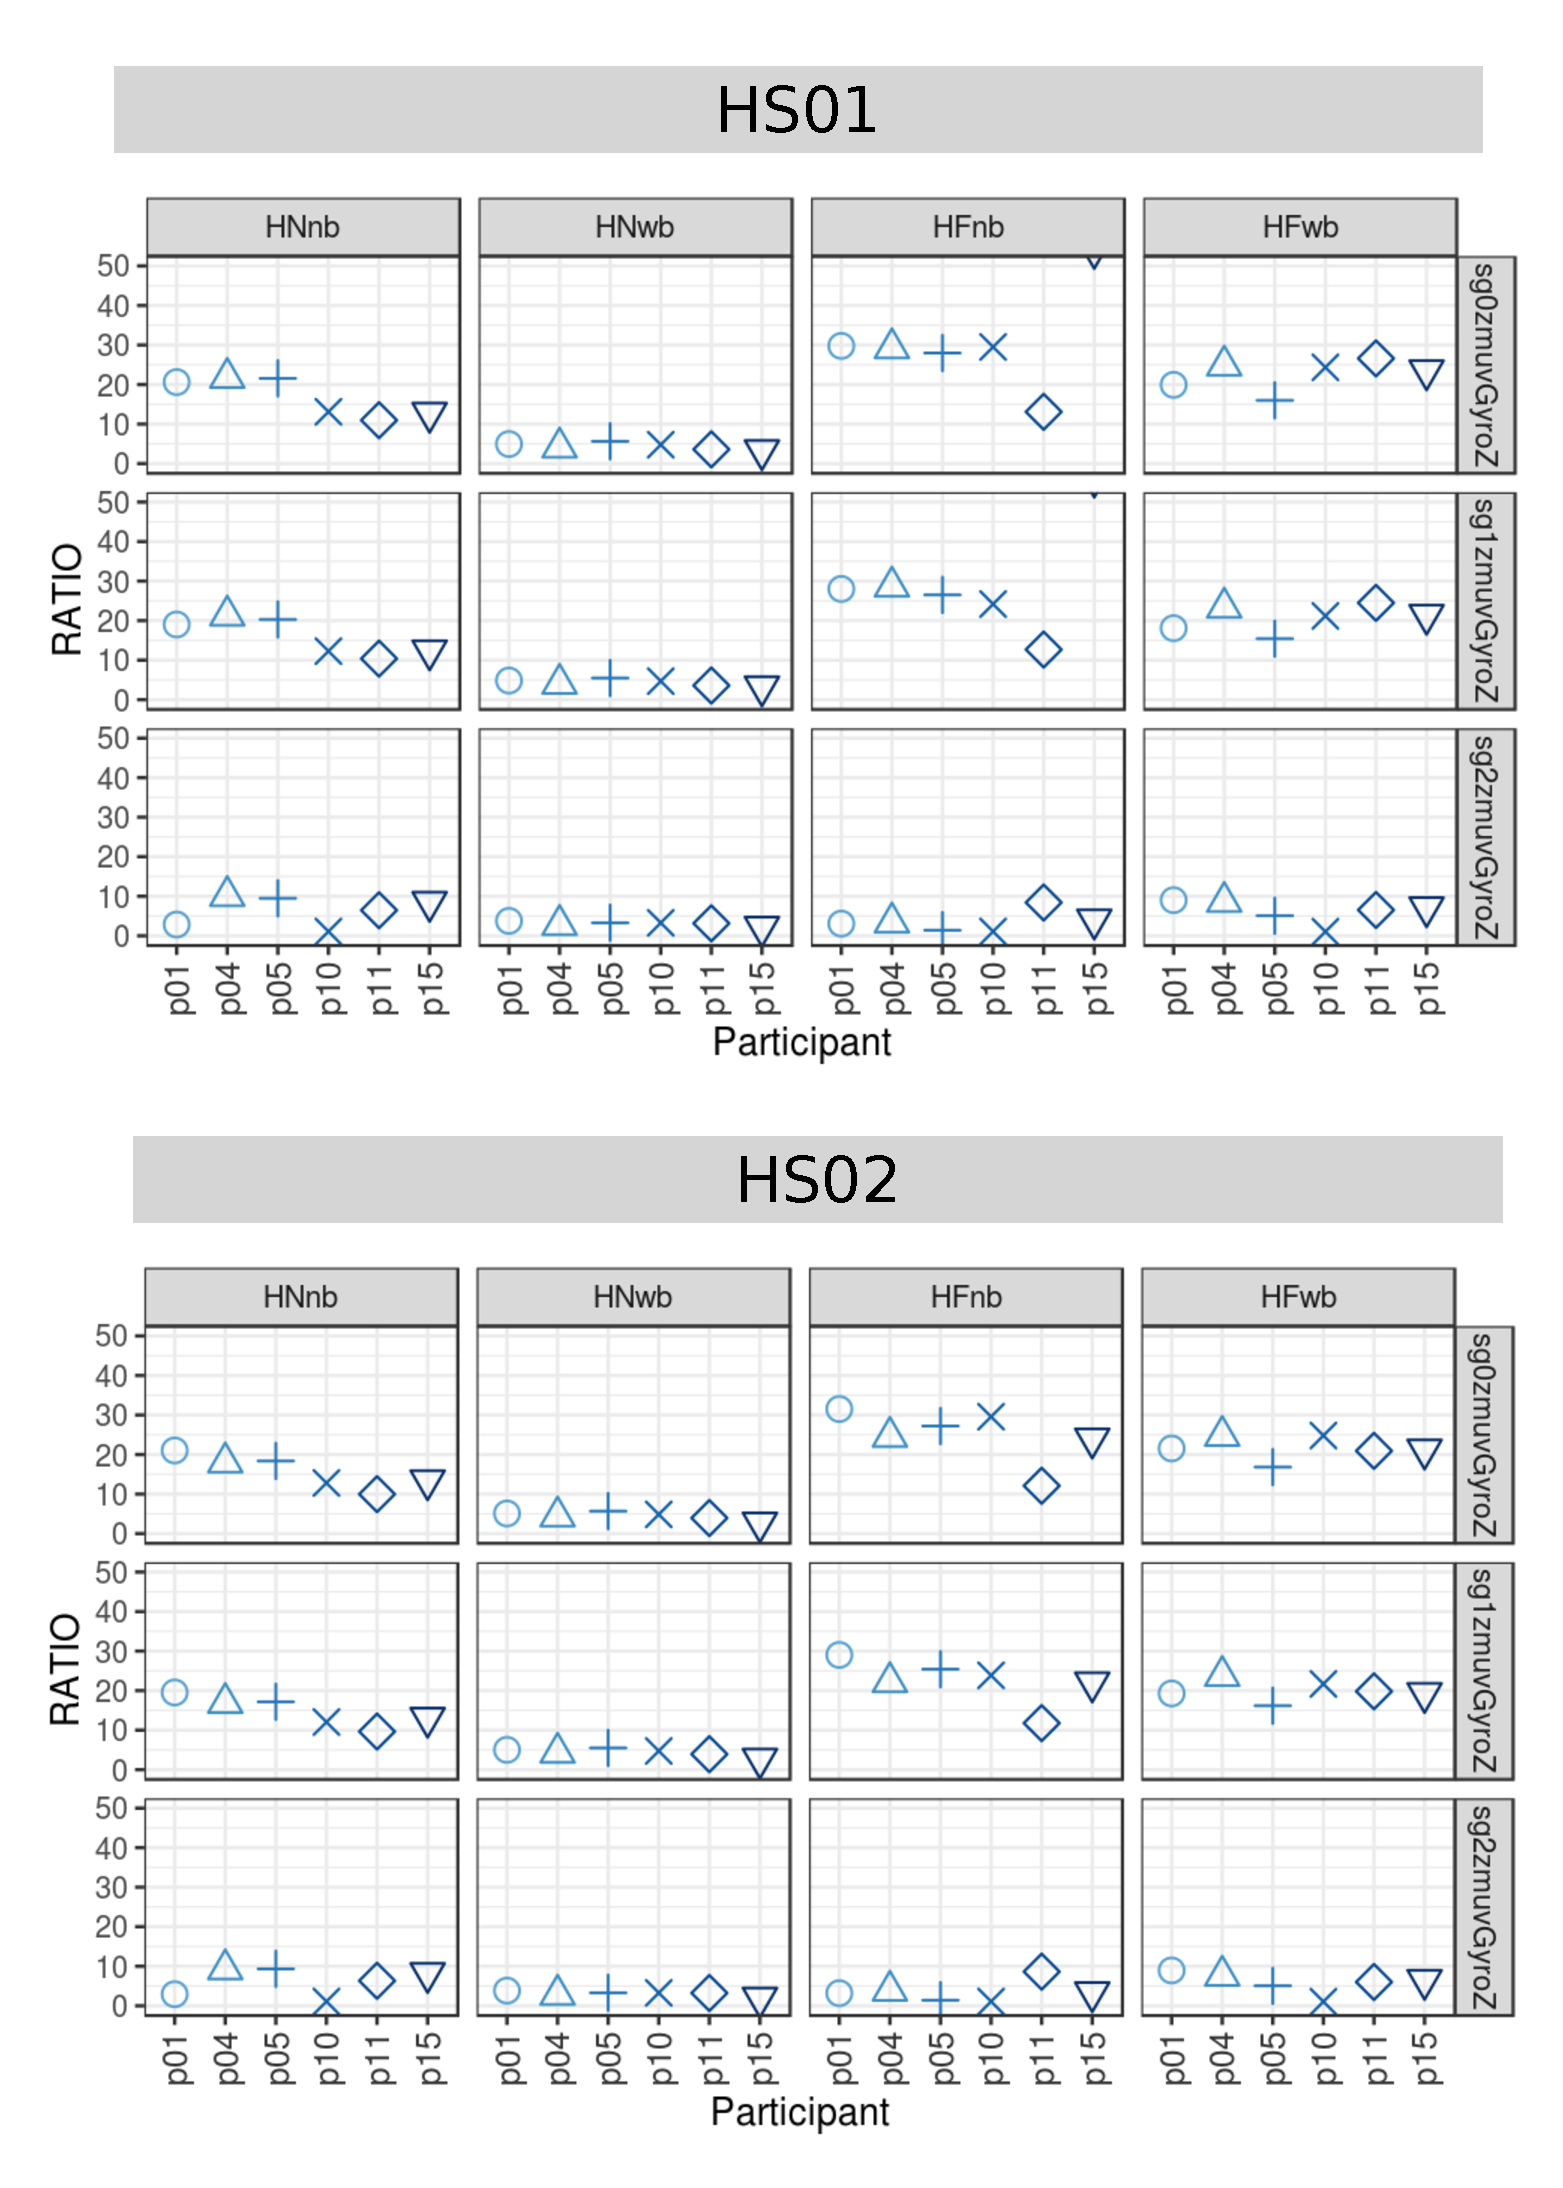
\includegraphics[width=0.9\textwidth]{rqa_ratio_H_w500}
    \caption
	[RATIO values for horizontal arm movements]{
	{\bf RATIO values for horizontal arm movements.}	
	RATIO values, representing dynamic transitions, 
	for 6 participants performing horizontal arm movements 
	(HNnb, HNwb, HFnb, HFwb)
	with sensors HS01, HS02 and three smoothed-normalised axis 
	of GyroZ (sg0zmuvGyroZ, sg1zmuvGyroZ and sg2zmuvGyroZ).
	RATIO values were computed with 
	embedding parameters $m=9$, $\tau=6$ and recurrence threshold
	$\epsilon=1$.
	R code to reproduce the figure is available from \cite{hwum2018}.
        }
    \label{fig:rqa_ratio_H}
\end{figure}
%%---------------------------------(FIGURE)------------------------------------
%%---------------------------------(FIGURE)------------------------------------
\begin{figure}
\centering
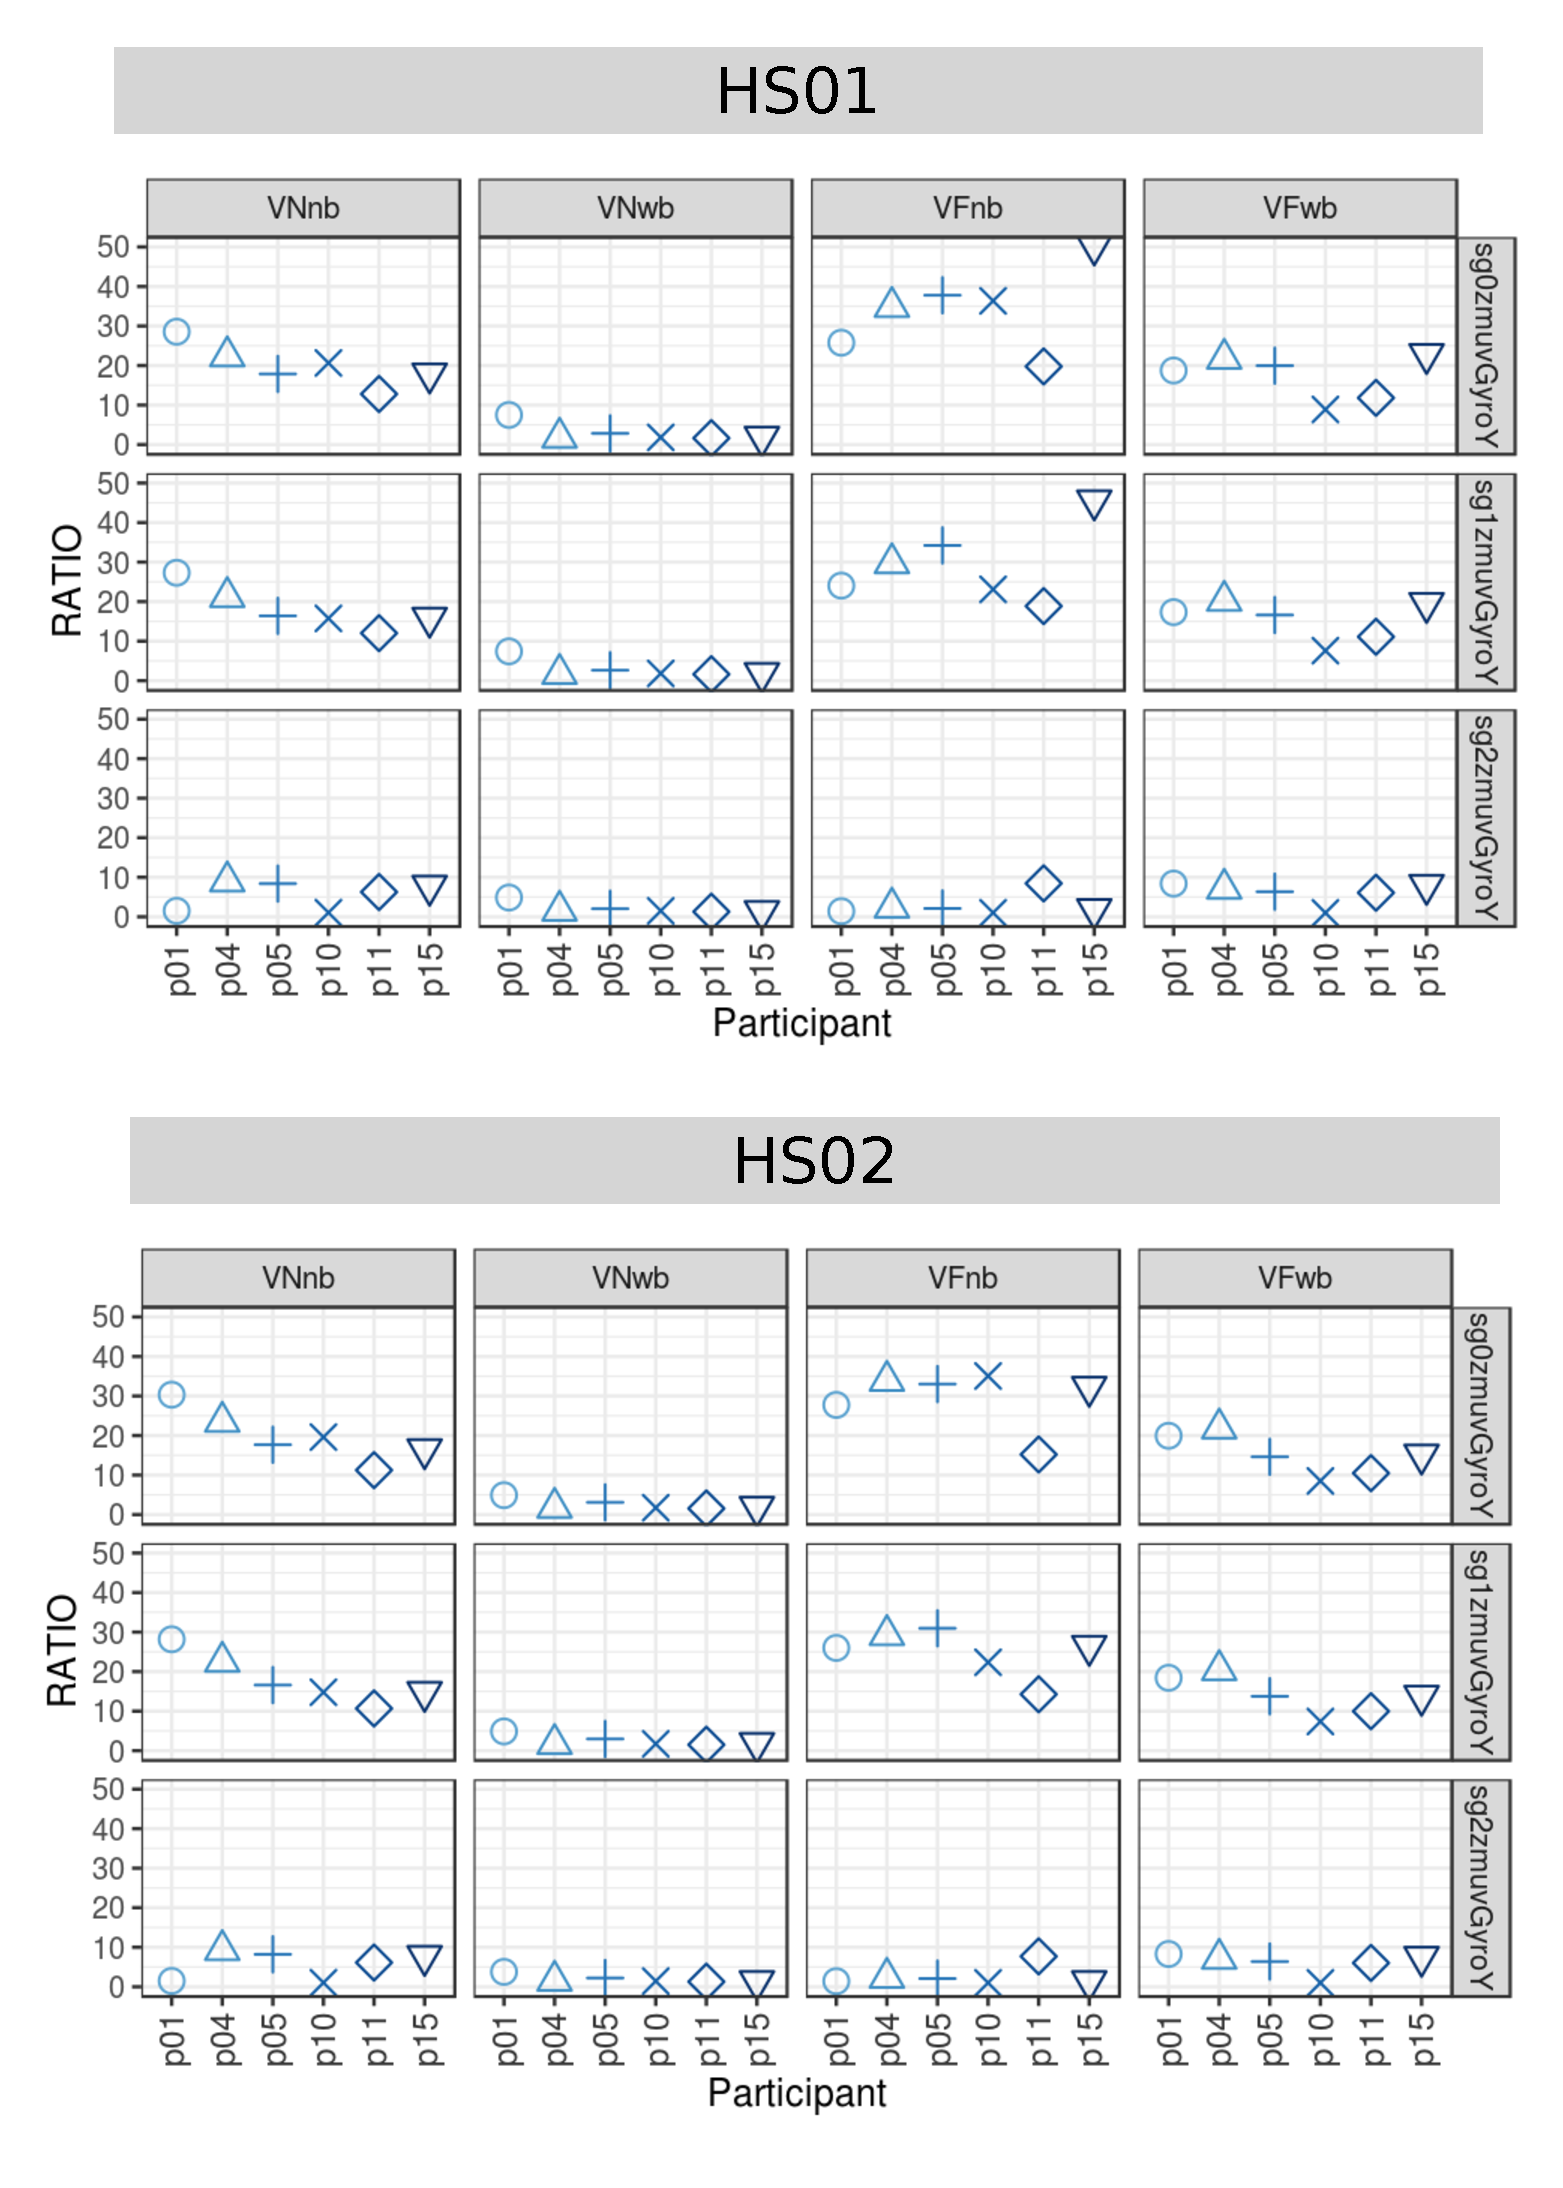
\includegraphics[width=0.9\textwidth]{rqa_ratio_V_w500}
    \caption
	[RATIO values for vertical arm movements]{
	{\bf RATIO values for vertical arm movements.}	
	RATIO values, representing dynamic transitions, 
	for 6 participants performing vertical arm movements 
	(VNnb, VNwb, VFnb, VFwb)
	with sensors HS01, HS02 and three smoothed-normalised axis 
	of GyroY (sg0zmuvGyroY, sg1zmuvGyroY and sg2zmuvGyroY).
	RATIO values were computed with 
	embedding parameters $m=9$, $\tau=6$ and recurrence threshold
	$\epsilon=1$.
	R code to reproduce the figure is available from \cite{hwum2018}.
        }
    \label{fig:rqa_ratio_V}
\end{figure}
%%---------------------------------(FIGURE)------------------------------------



\newpage
\subsection{ENTR values}
ENTR values for horizontal and vertical arm movements are shown 
in Figs \ref{fig:rqa_entr_H} and \ref{fig:rqa_entr_V}.

Figs \ref{fig:rqa_entr_H} show ENTR values for horizontal arm movements.
ENTR values appear to be similar for sg0zmuvGyroZ and sg1zmuvGyroZ 
and oscillate between 2 to 4, while ENTR values for sg2zmuvGyroZ appear 
to show similar fluctuations but with higher ENTR values oscillating 
between 3.5 to 5  with the exception of $p10$ with activities VNnb and VFwb 
for sg2zmuvGyroY which ENTR values are slightly out of range.
ENTR values appear to be similar for sensor HS01 and HS02.

Figs \ref{fig:rqa_entr_V} show ENTR values for vertical arm movements.
ENTR values for sg0zmuvGyroY and sg1zmuvGyroY appear to show the same
values and oscillate between 2 to 4, while ENTR values appear to oscillate
between 3.5 to 5 with the exception of $p10$ with activities VNnb and VFwb 
for sg2zmuvGyroY which ENTR values are out of range.
ENTR values for sensor HS01 and HS02 appear to show the same values. 




%%---------------------------------(FIGURE)------------------------------------
\begin{figure}
\centering
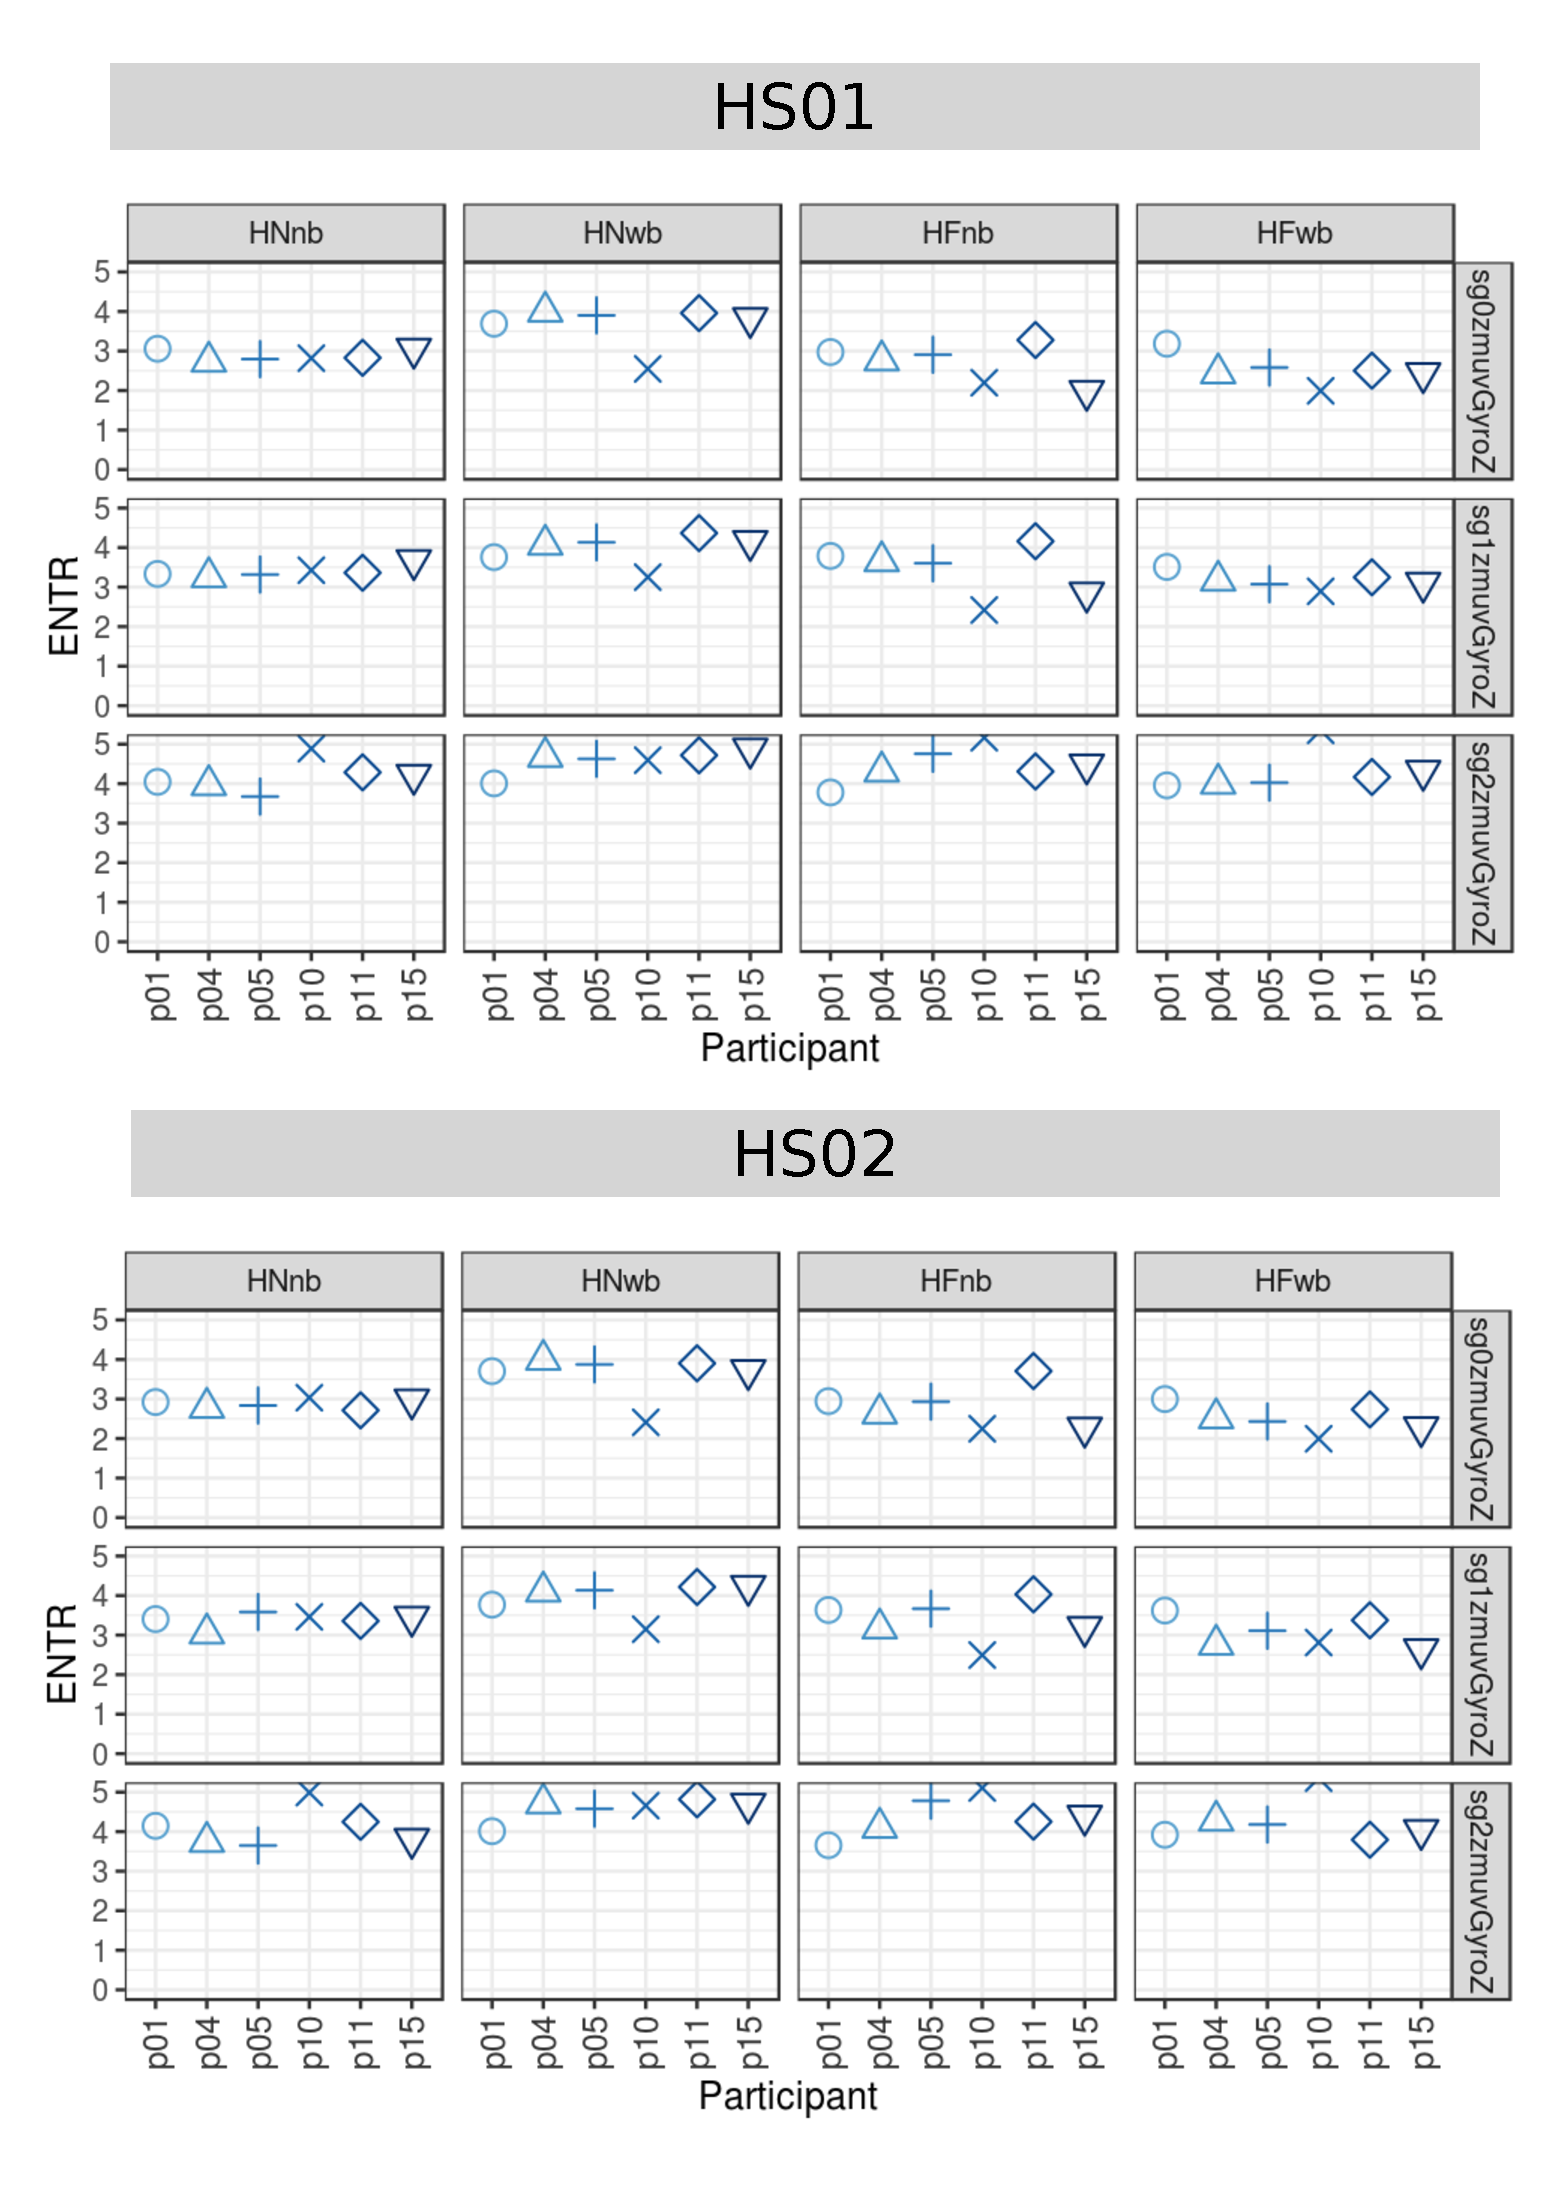
\includegraphics[width=0.88\textwidth]{rqa_entr_H_w500}
    \caption
	[ENTR values for horizontal arm movements]{
	{\bf ENTR values for horizontal arm movements.}
	ENTR values (representing the complexity of the deterministic 
	structure in time series) for 
	6 participants performing horizontal arm movements 
	(HNnb, HNwb, HFnb, HFwb)
	for sensors HS01, HS02 and three smoothed-normalised axis 
	of GyroZ (sg0zmuvGyroZ, sg1zmuvGyroZ and sg2zmuvGyroZ).
	ENTR values were computed with 
	embedding parameters $m=9$, $\tau=6$ and recurrence threshold
	$\epsilon=1$.
	R code to reproduce the figure is available from \cite{hwum2018}.
        }
    \label{fig:rqa_entr_H}
\end{figure}
%%---------------------------------(FIGURE)------------------------------------
%%---------------------------------(FIGURE)------------------------------------
\begin{figure}
\centering
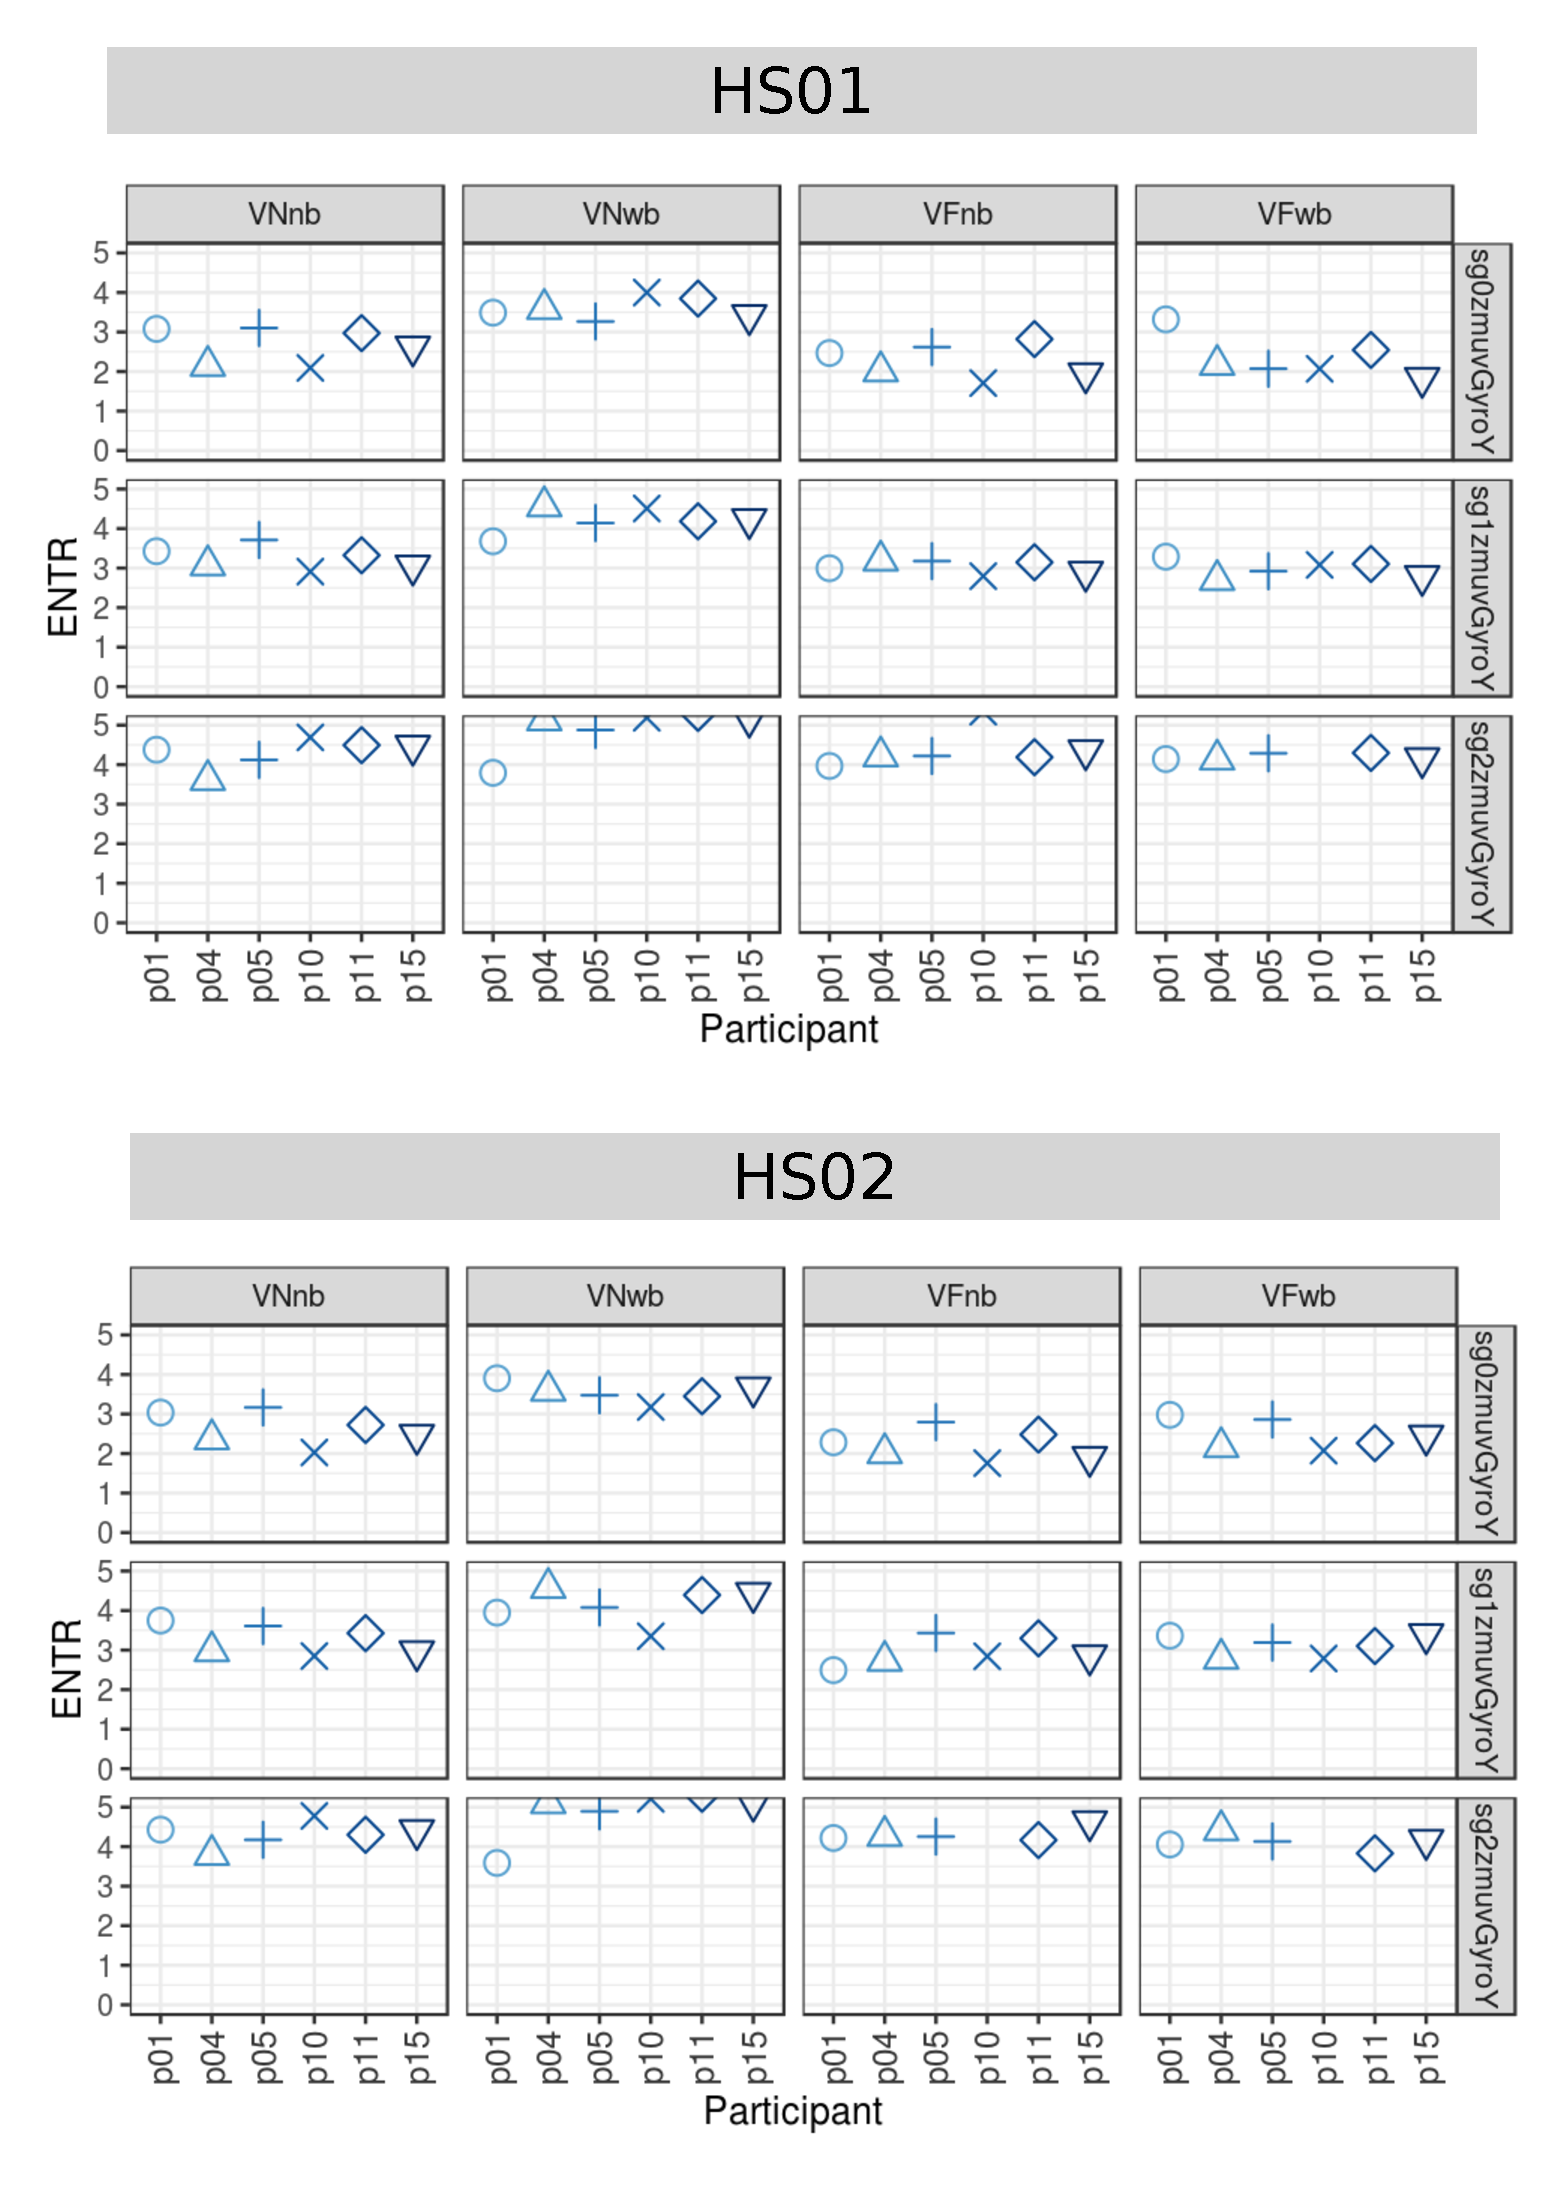
\includegraphics[width=0.88\textwidth]{rqa_entr_V_w500}
    \caption
	[ENTR values for vertical arm movements]{
	{\bf ENTR values for vertical arm movements.}	
	ENTR values (representing the complexity of the deterministic 
	structure in time series) for 
	6 participants performing vertical arm movements (VNnb, VNwb, VFnb, VFwb)
	for sensors HS01, HS02 and three smoothed-normalised axis 
	of GyroY (sg0zmuvGyroY, sg1zmuvGyroY and sg2zmuvGyroY).
	ENTR values were computed with 
	embedding parameters $m=9$, $\tau=6$ and recurrence threshold
	$\epsilon=1$.
	R code to reproduce the figure is available from \cite{hwum2018}.
        }
    \label{fig:rqa_entr_V}
\end{figure}
%%---------------------------------(FIGURE)------------------------------------





